
\chapter{Extended Result}
\FloatBarrier
\section{Set Estimation}\label{eresult:setest}
\FloatBarrier
Estimation using the techniques with different models are illustrated using data for one particular vehicle in the dataset in this chapter. Results show that the true state is always bounded by the set of estimation. For acceleration, there is no true measurement because the acceleration of the tracked vehicle is absent in the dataset.

\subsection{Segment Minimization using F-Radius}
\FloatBarrier
\begin{figure}[h]
\hspace*{\fill} 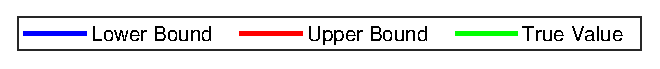
\includegraphics[scale=0.8]{figures/legend}\\\\
\begin{subfigure}{.5\linewidth}
\centering
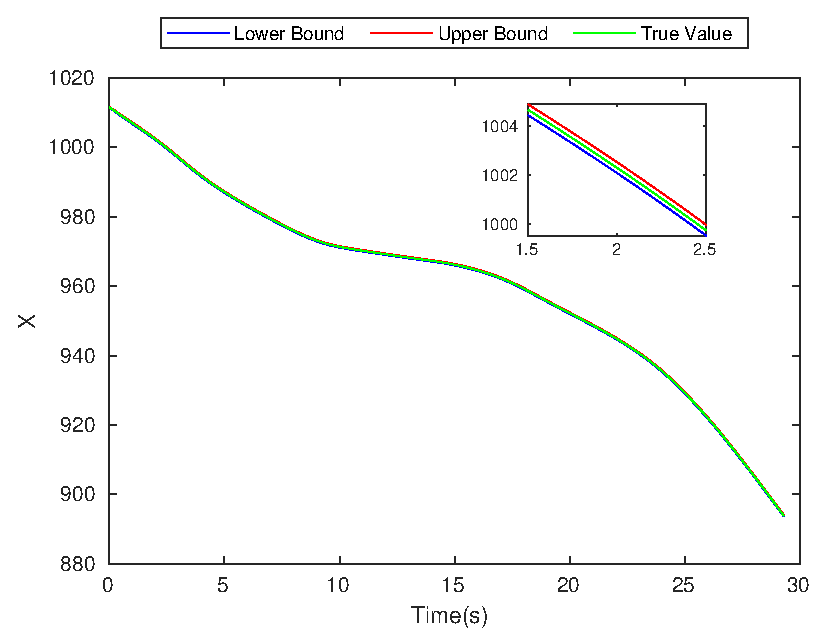
\includegraphics[width=\linewidth]{figures/Frad/s3cvSMX}
\end{subfigure}
\begin{subfigure}{.5\linewidth}
\centering
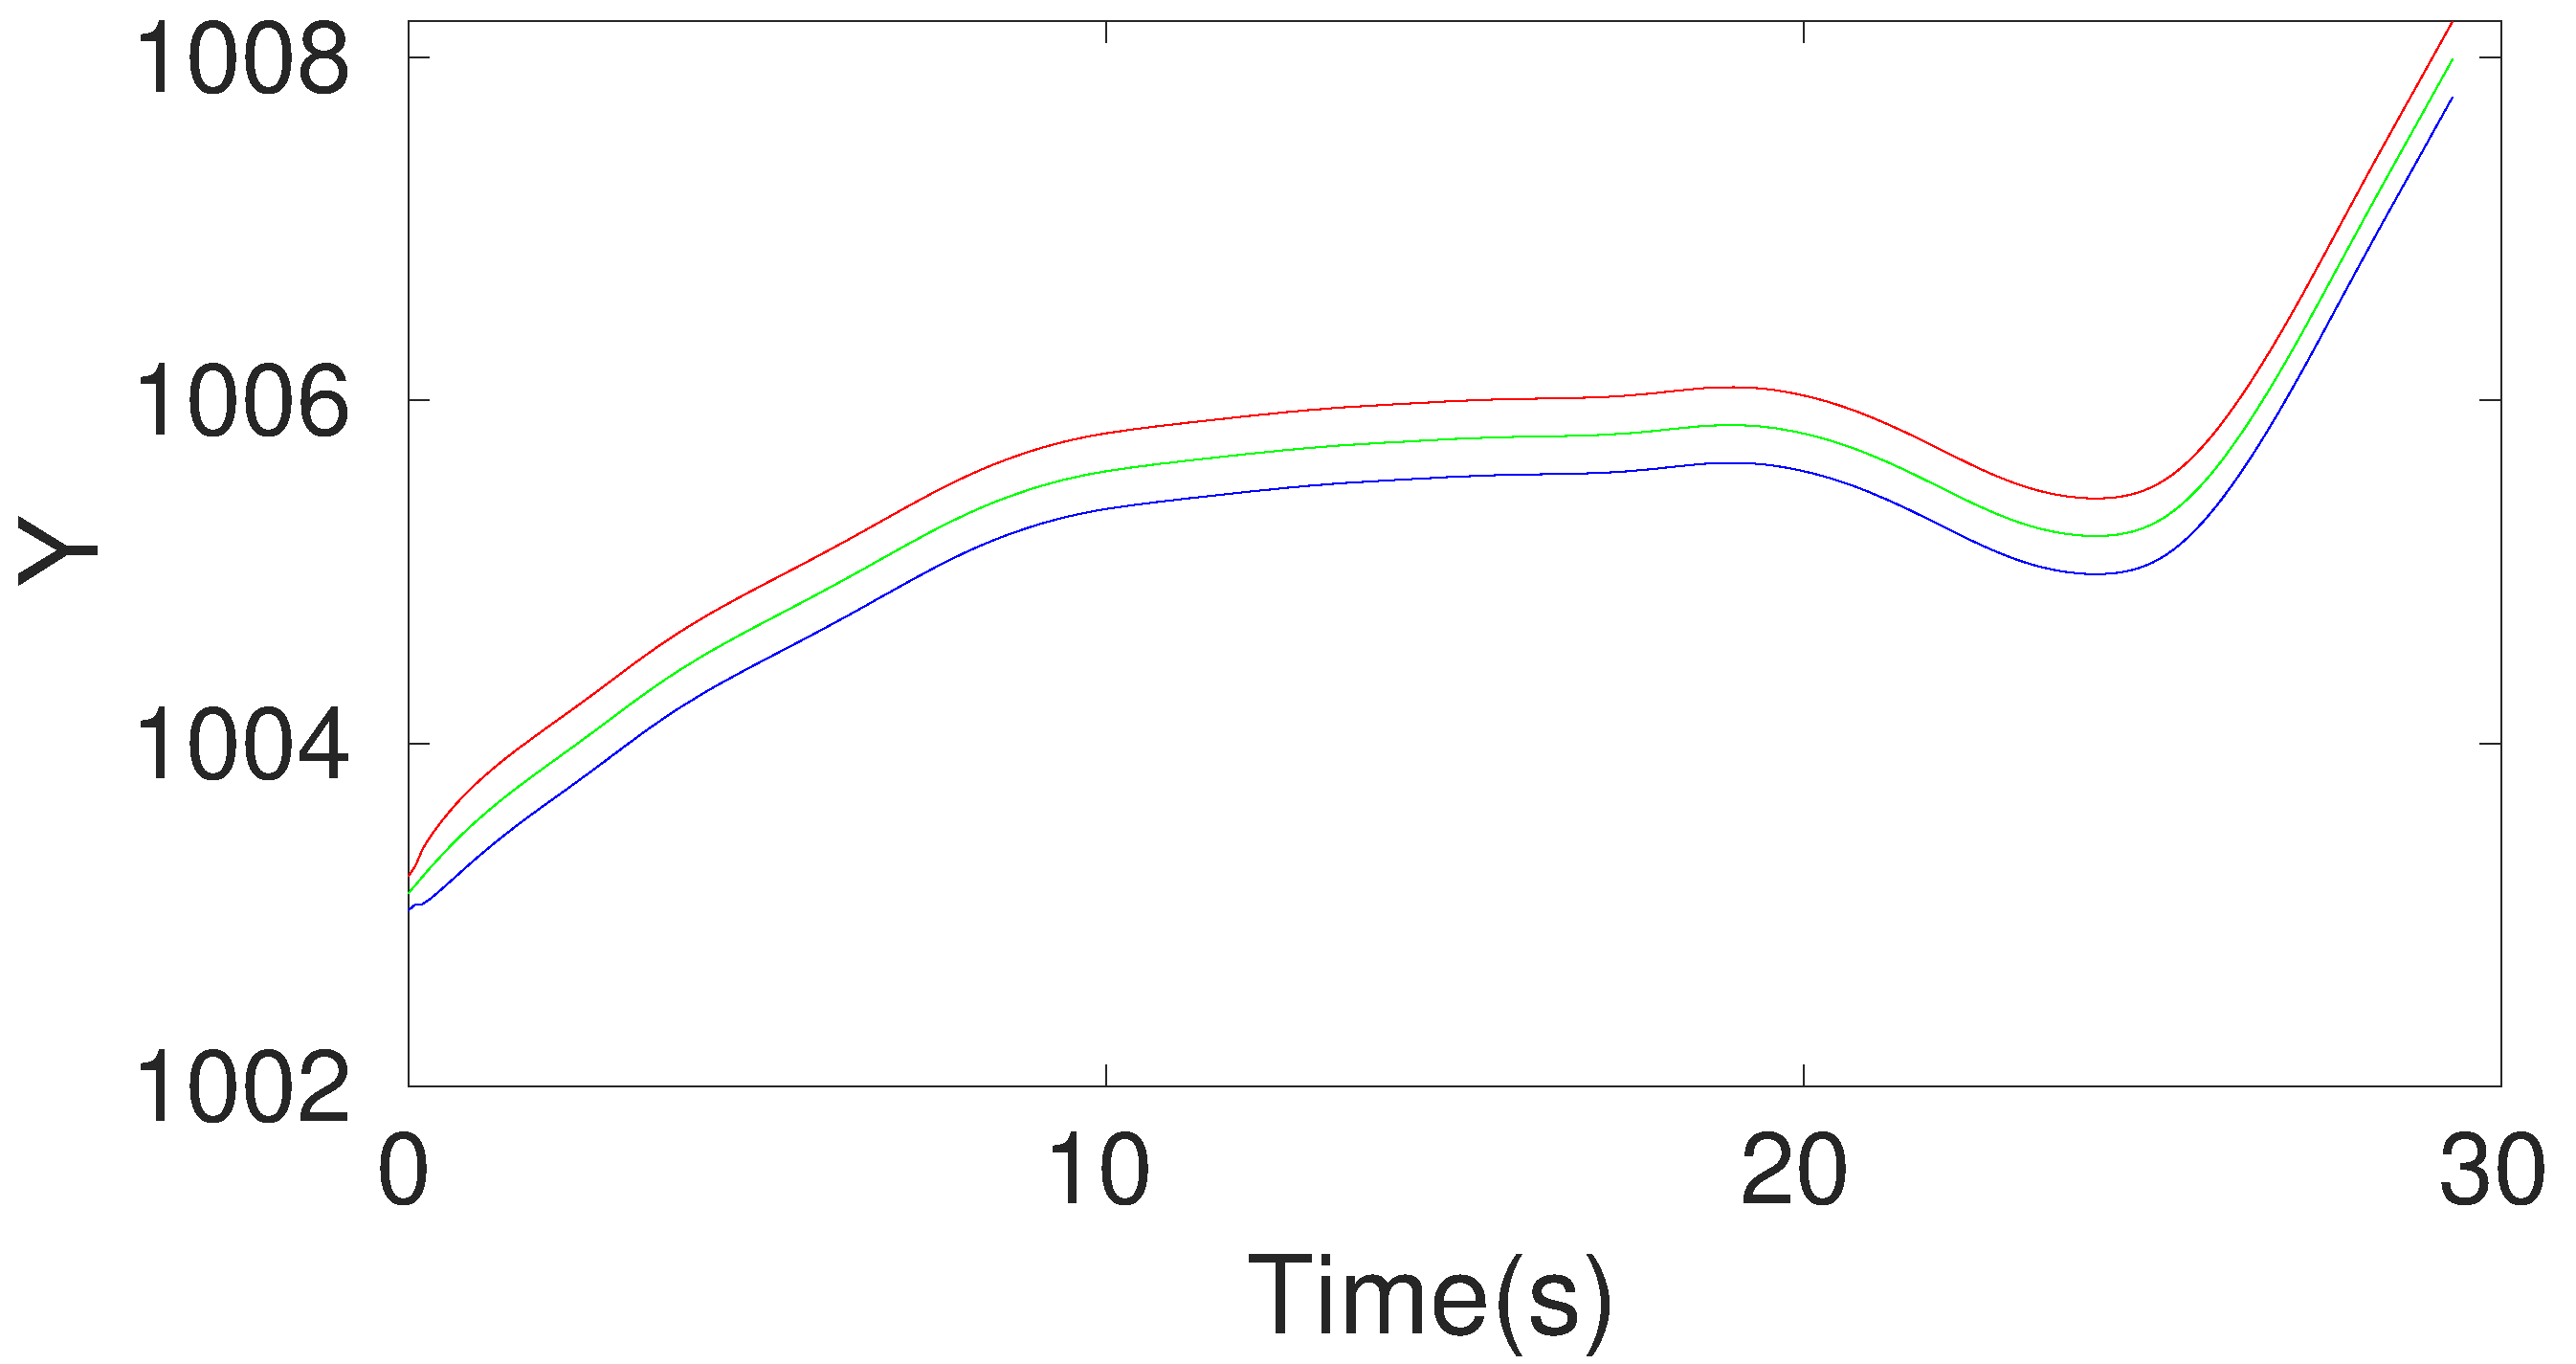
\includegraphics[width=\linewidth]{figures/Frad/s3cvSMY}
\end{subfigure}
\begin{subfigure}{.5\linewidth}
\centering
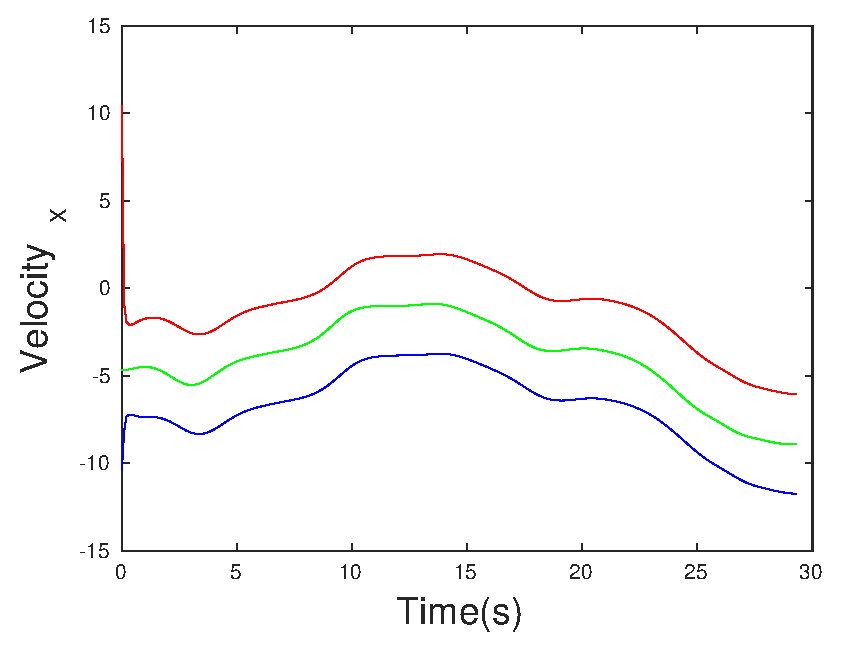
\includegraphics[width=\linewidth]{figures/Frad/s3cvSMVelocity_x}
\end{subfigure}
\begin{subfigure}{.5\linewidth}
\centering
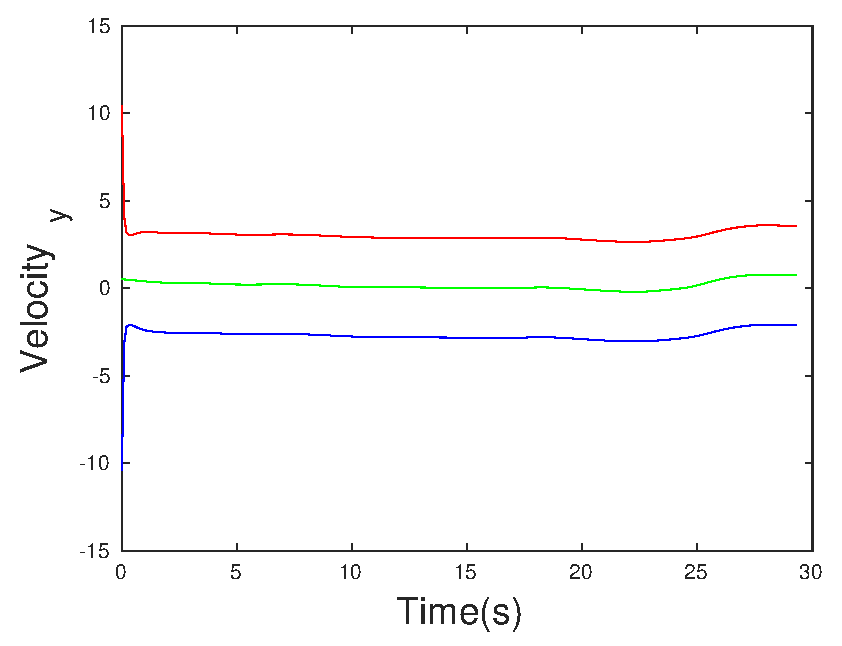
\includegraphics[width=\linewidth]{figures/Frad/s3cvSMVelocity_y}
\end{subfigure}
\caption{Estimation using the F-radius and the constant velocity model}
\end{figure}

\begin{figure}[h]
\hspace*{\fill} 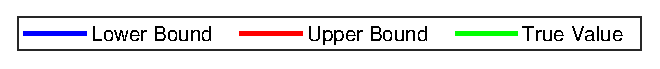
\includegraphics[scale=0.8]{figures/legend}\\\\
\begin{subfigure}{.5\linewidth}
\centering
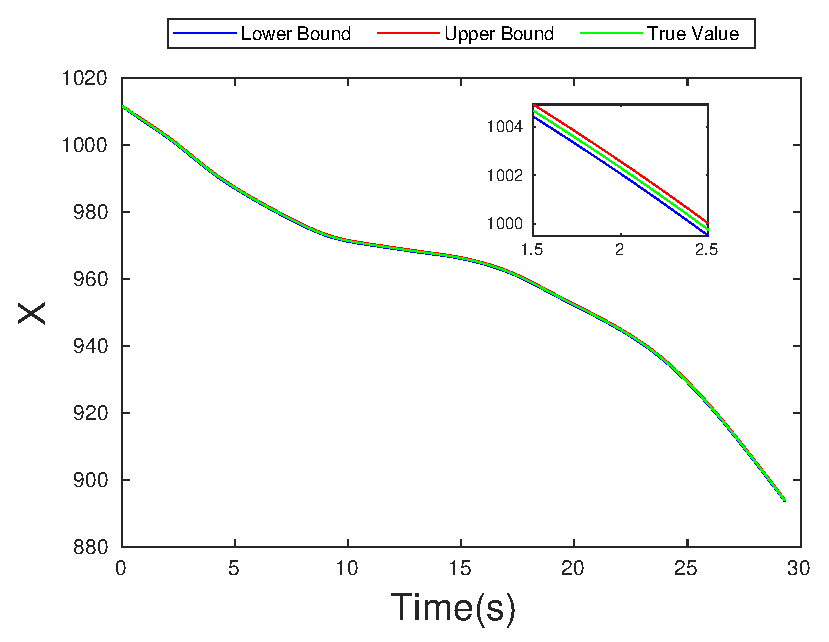
\includegraphics[width=\linewidth]{figures/Frad/s3caSMX}
\end{subfigure}
\begin{subfigure}{.5\linewidth}
\centering
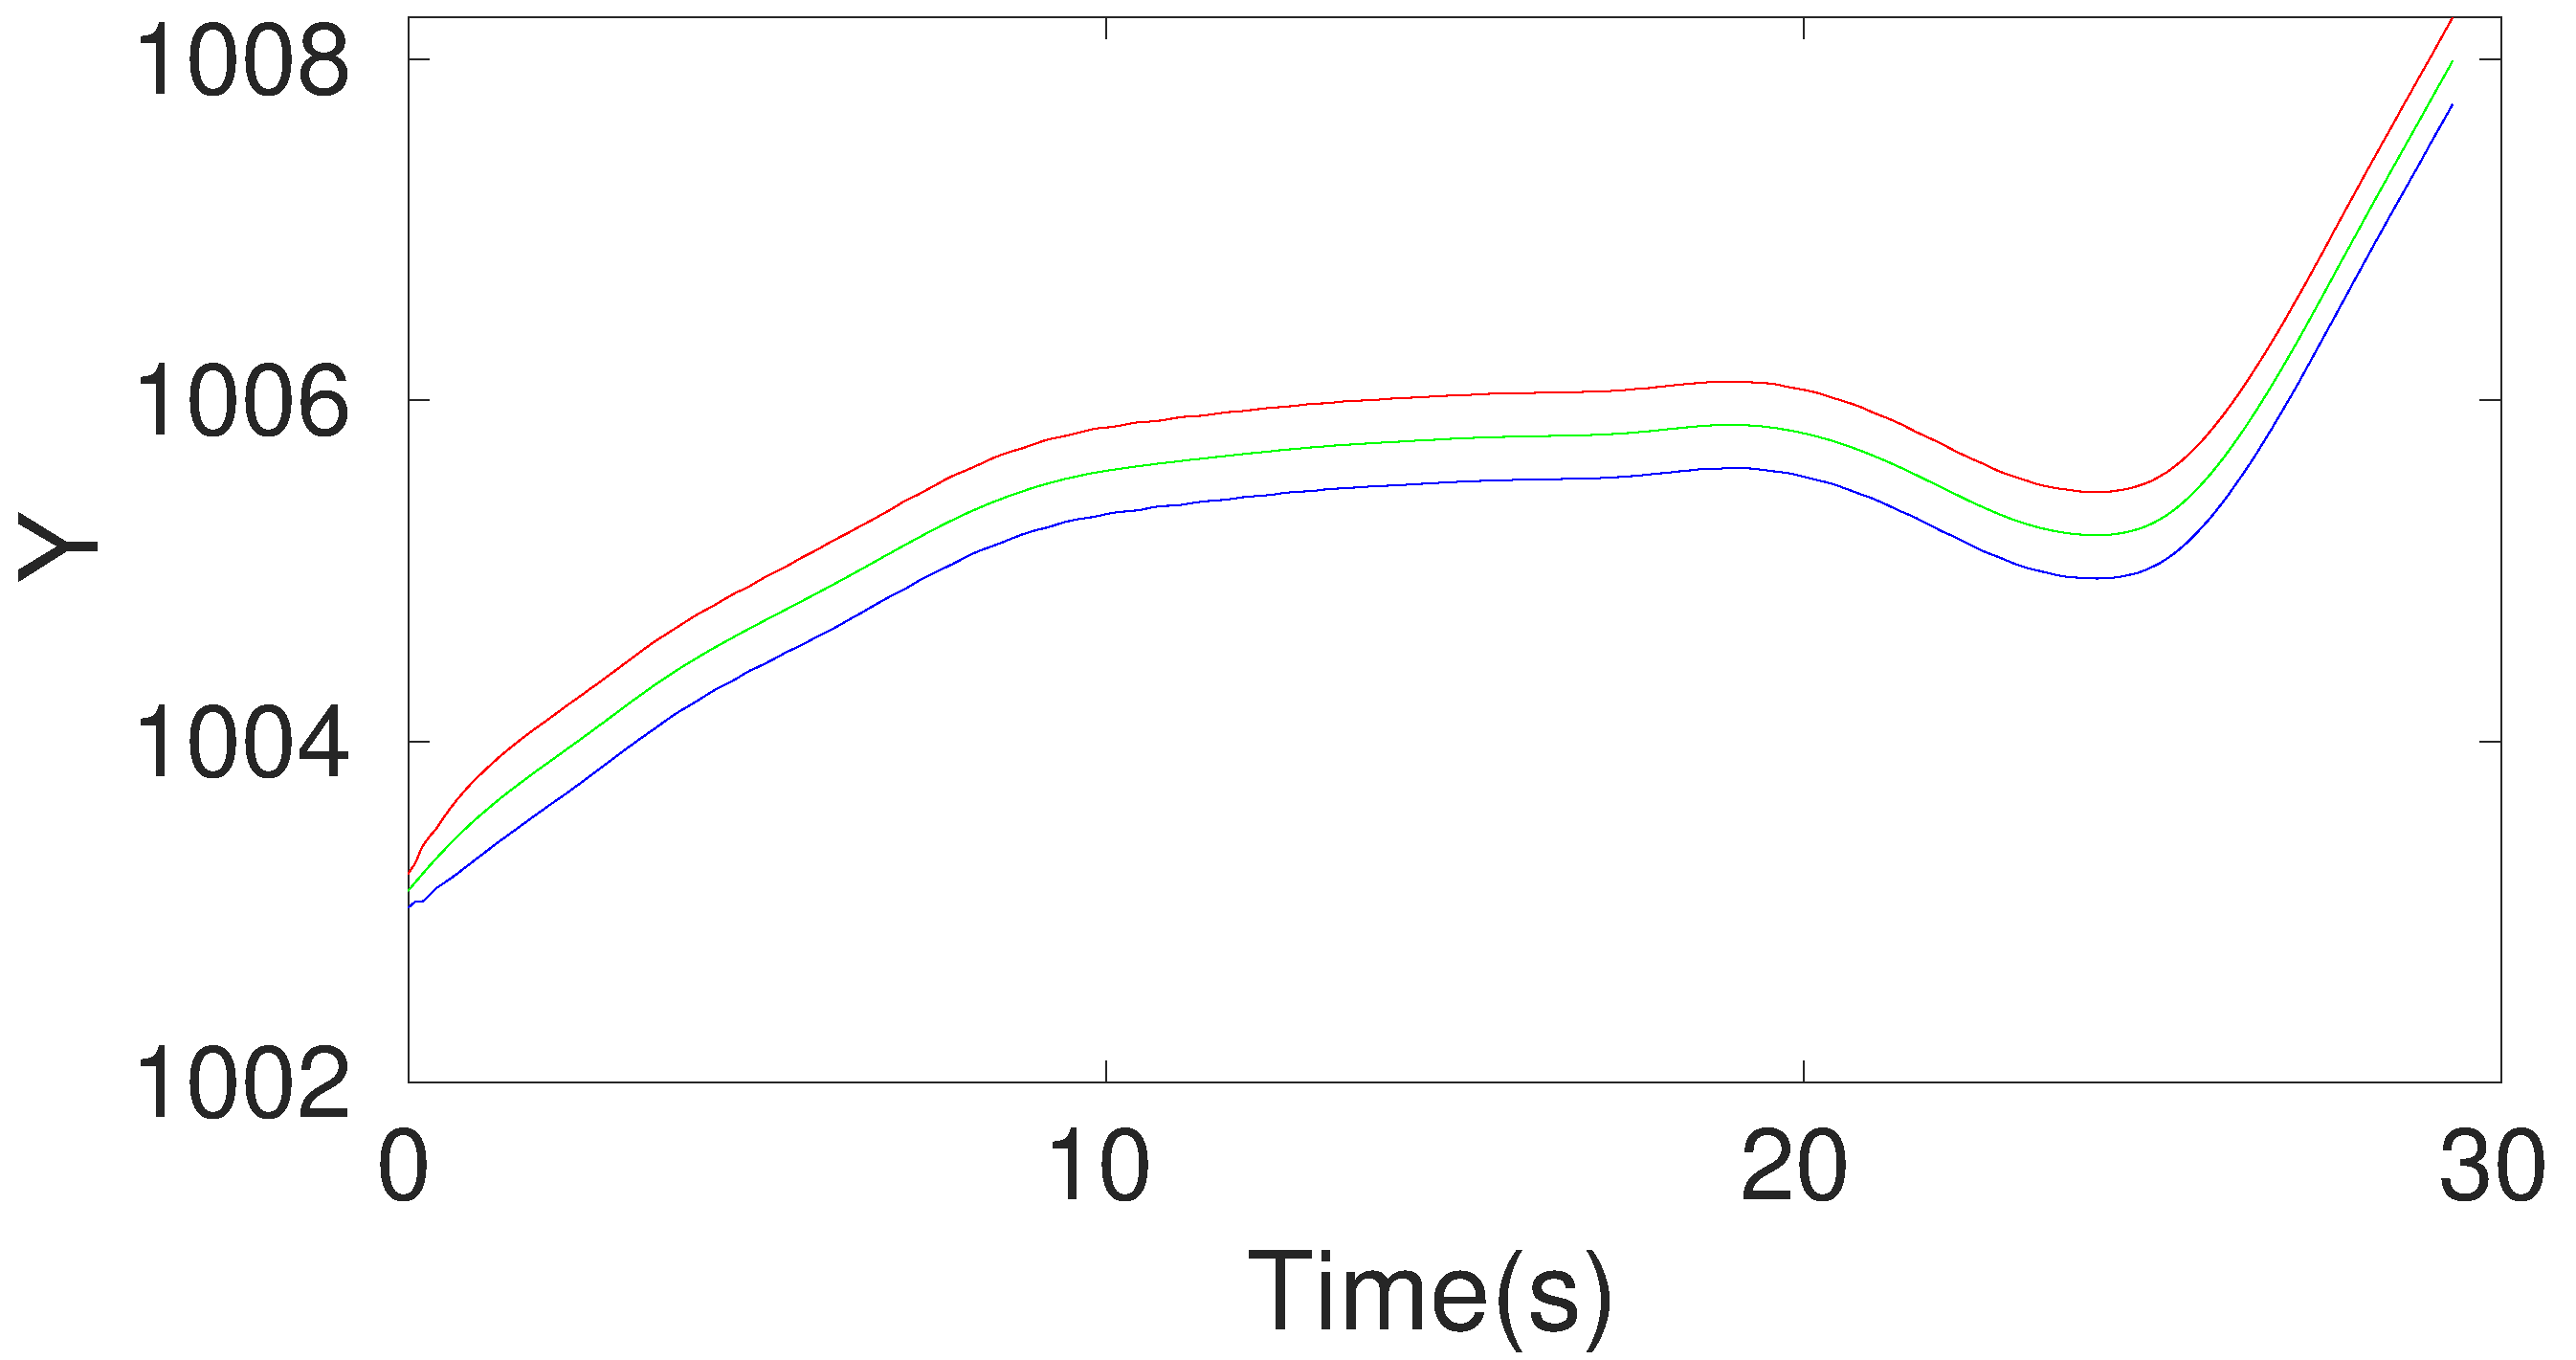
\includegraphics[width=\linewidth]{figures/Frad/s3caSMY}
\end{subfigure}
\begin{subfigure}{.5\linewidth}
\centering
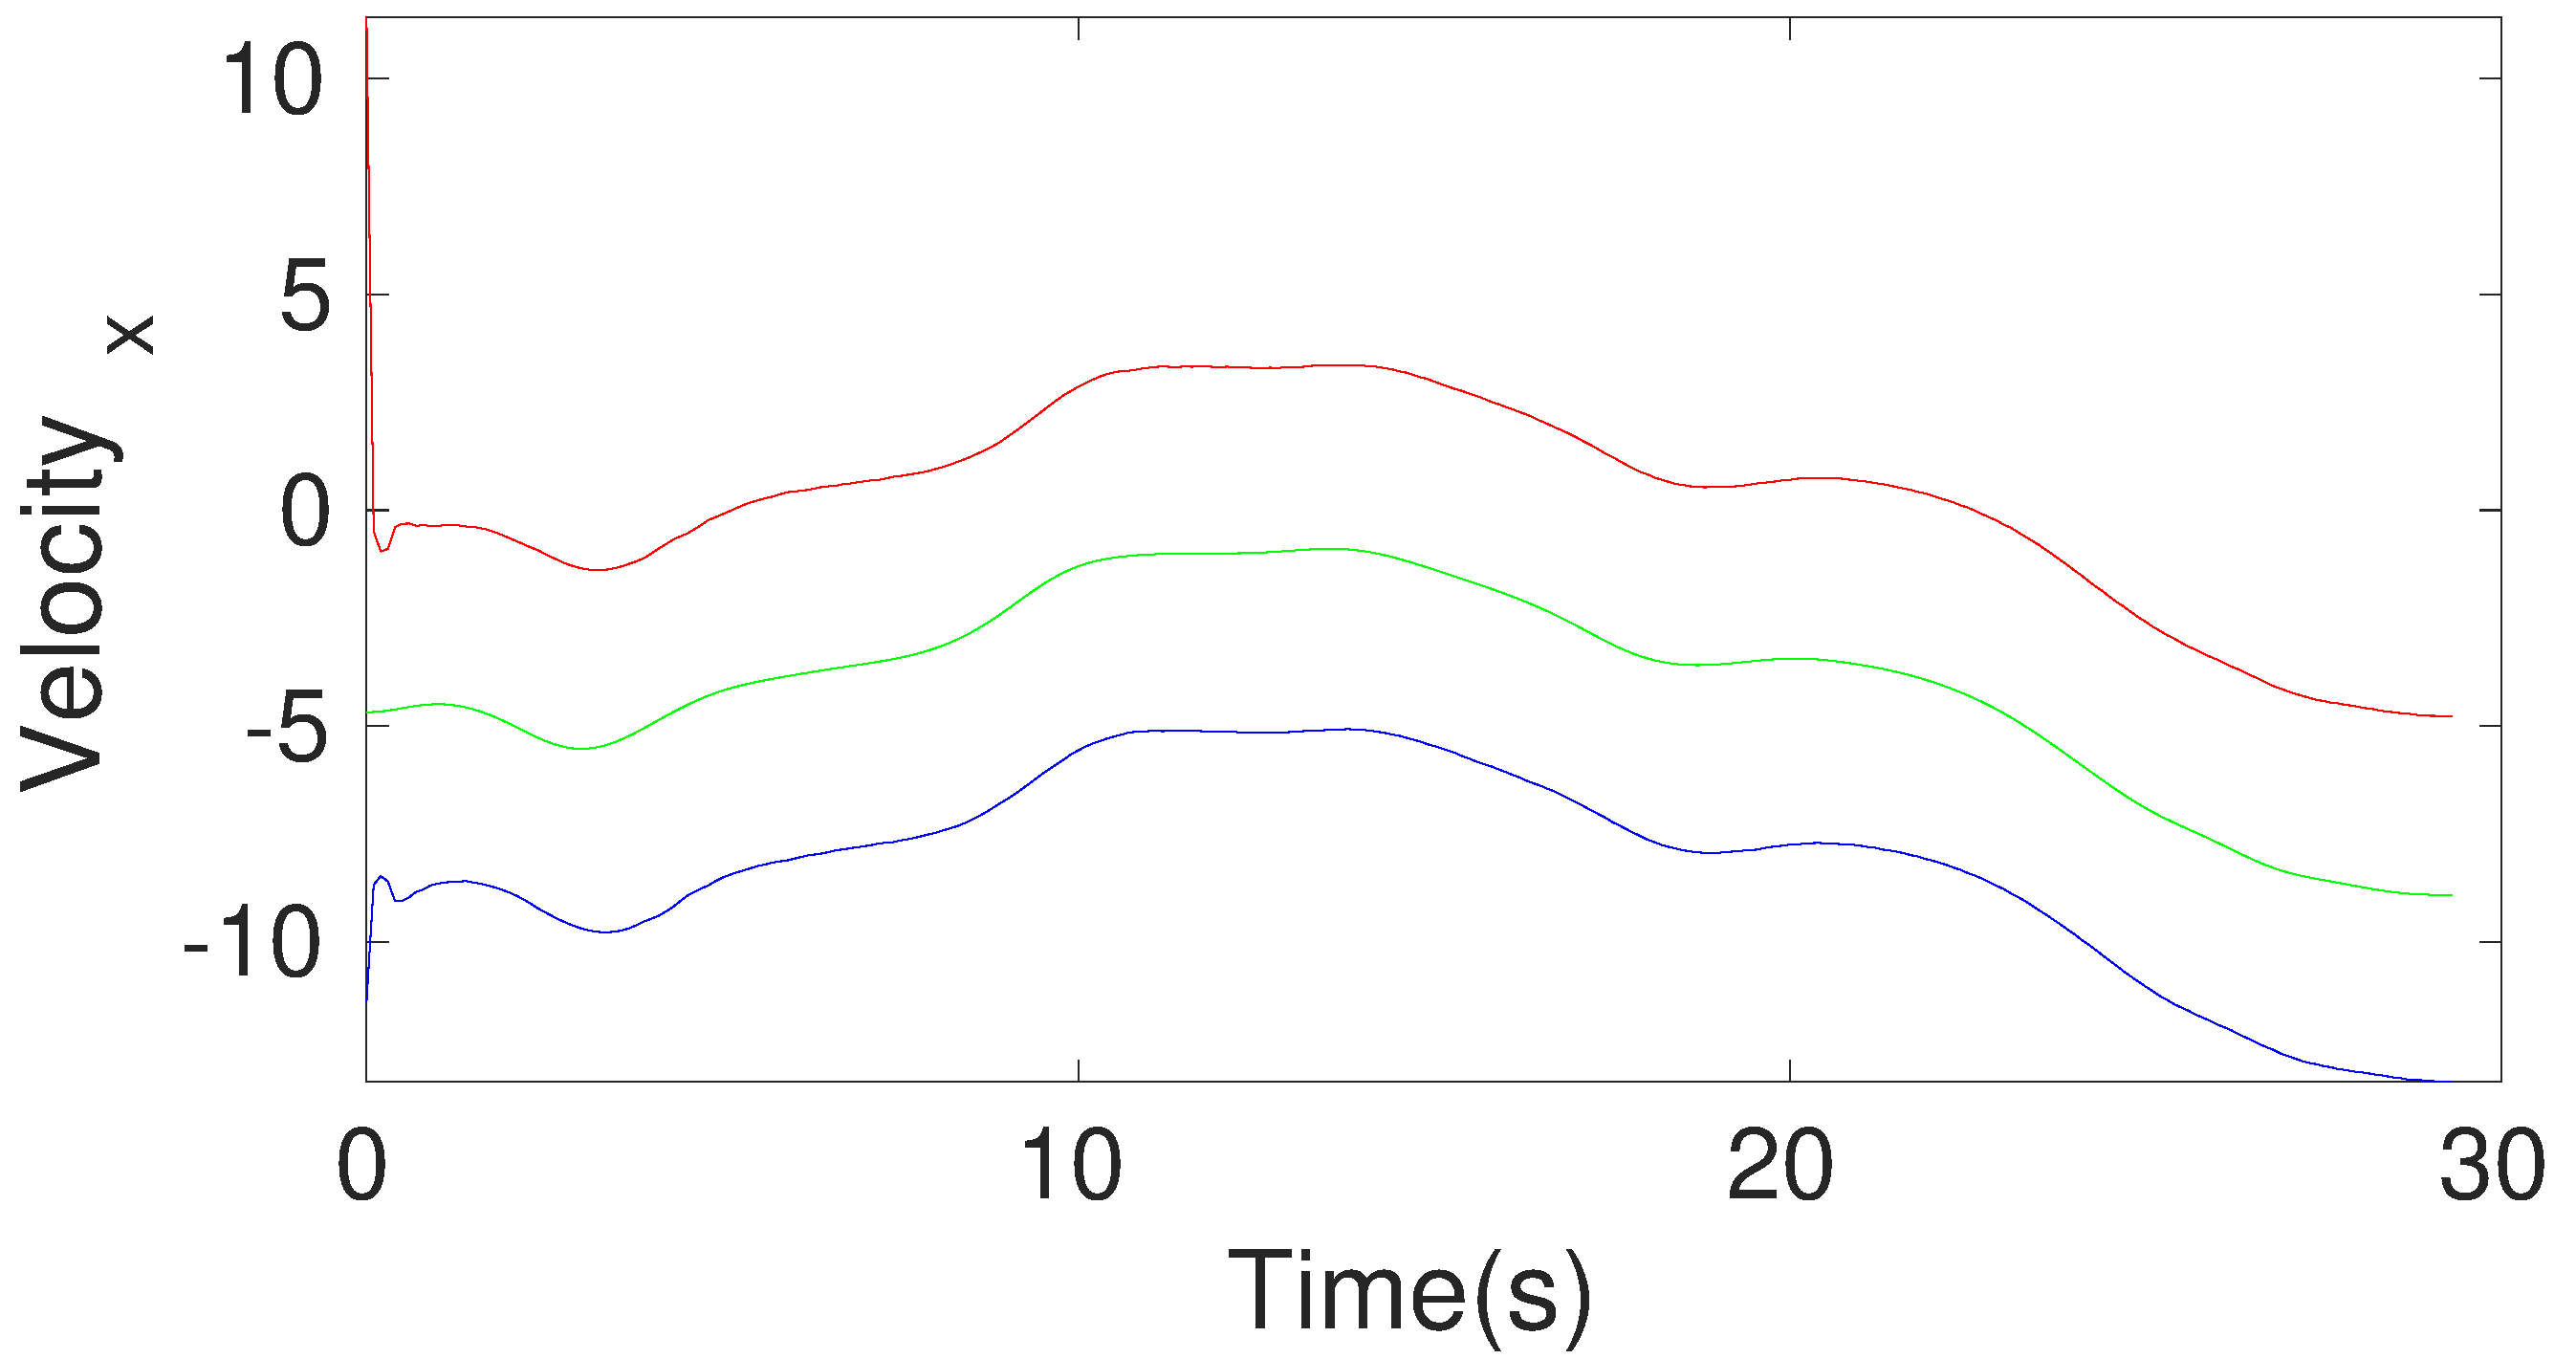
\includegraphics[width=\linewidth]{figures/Frad/s3caSMVelocity_x}
\end{subfigure}
\begin{subfigure}{.5\linewidth}
\centering
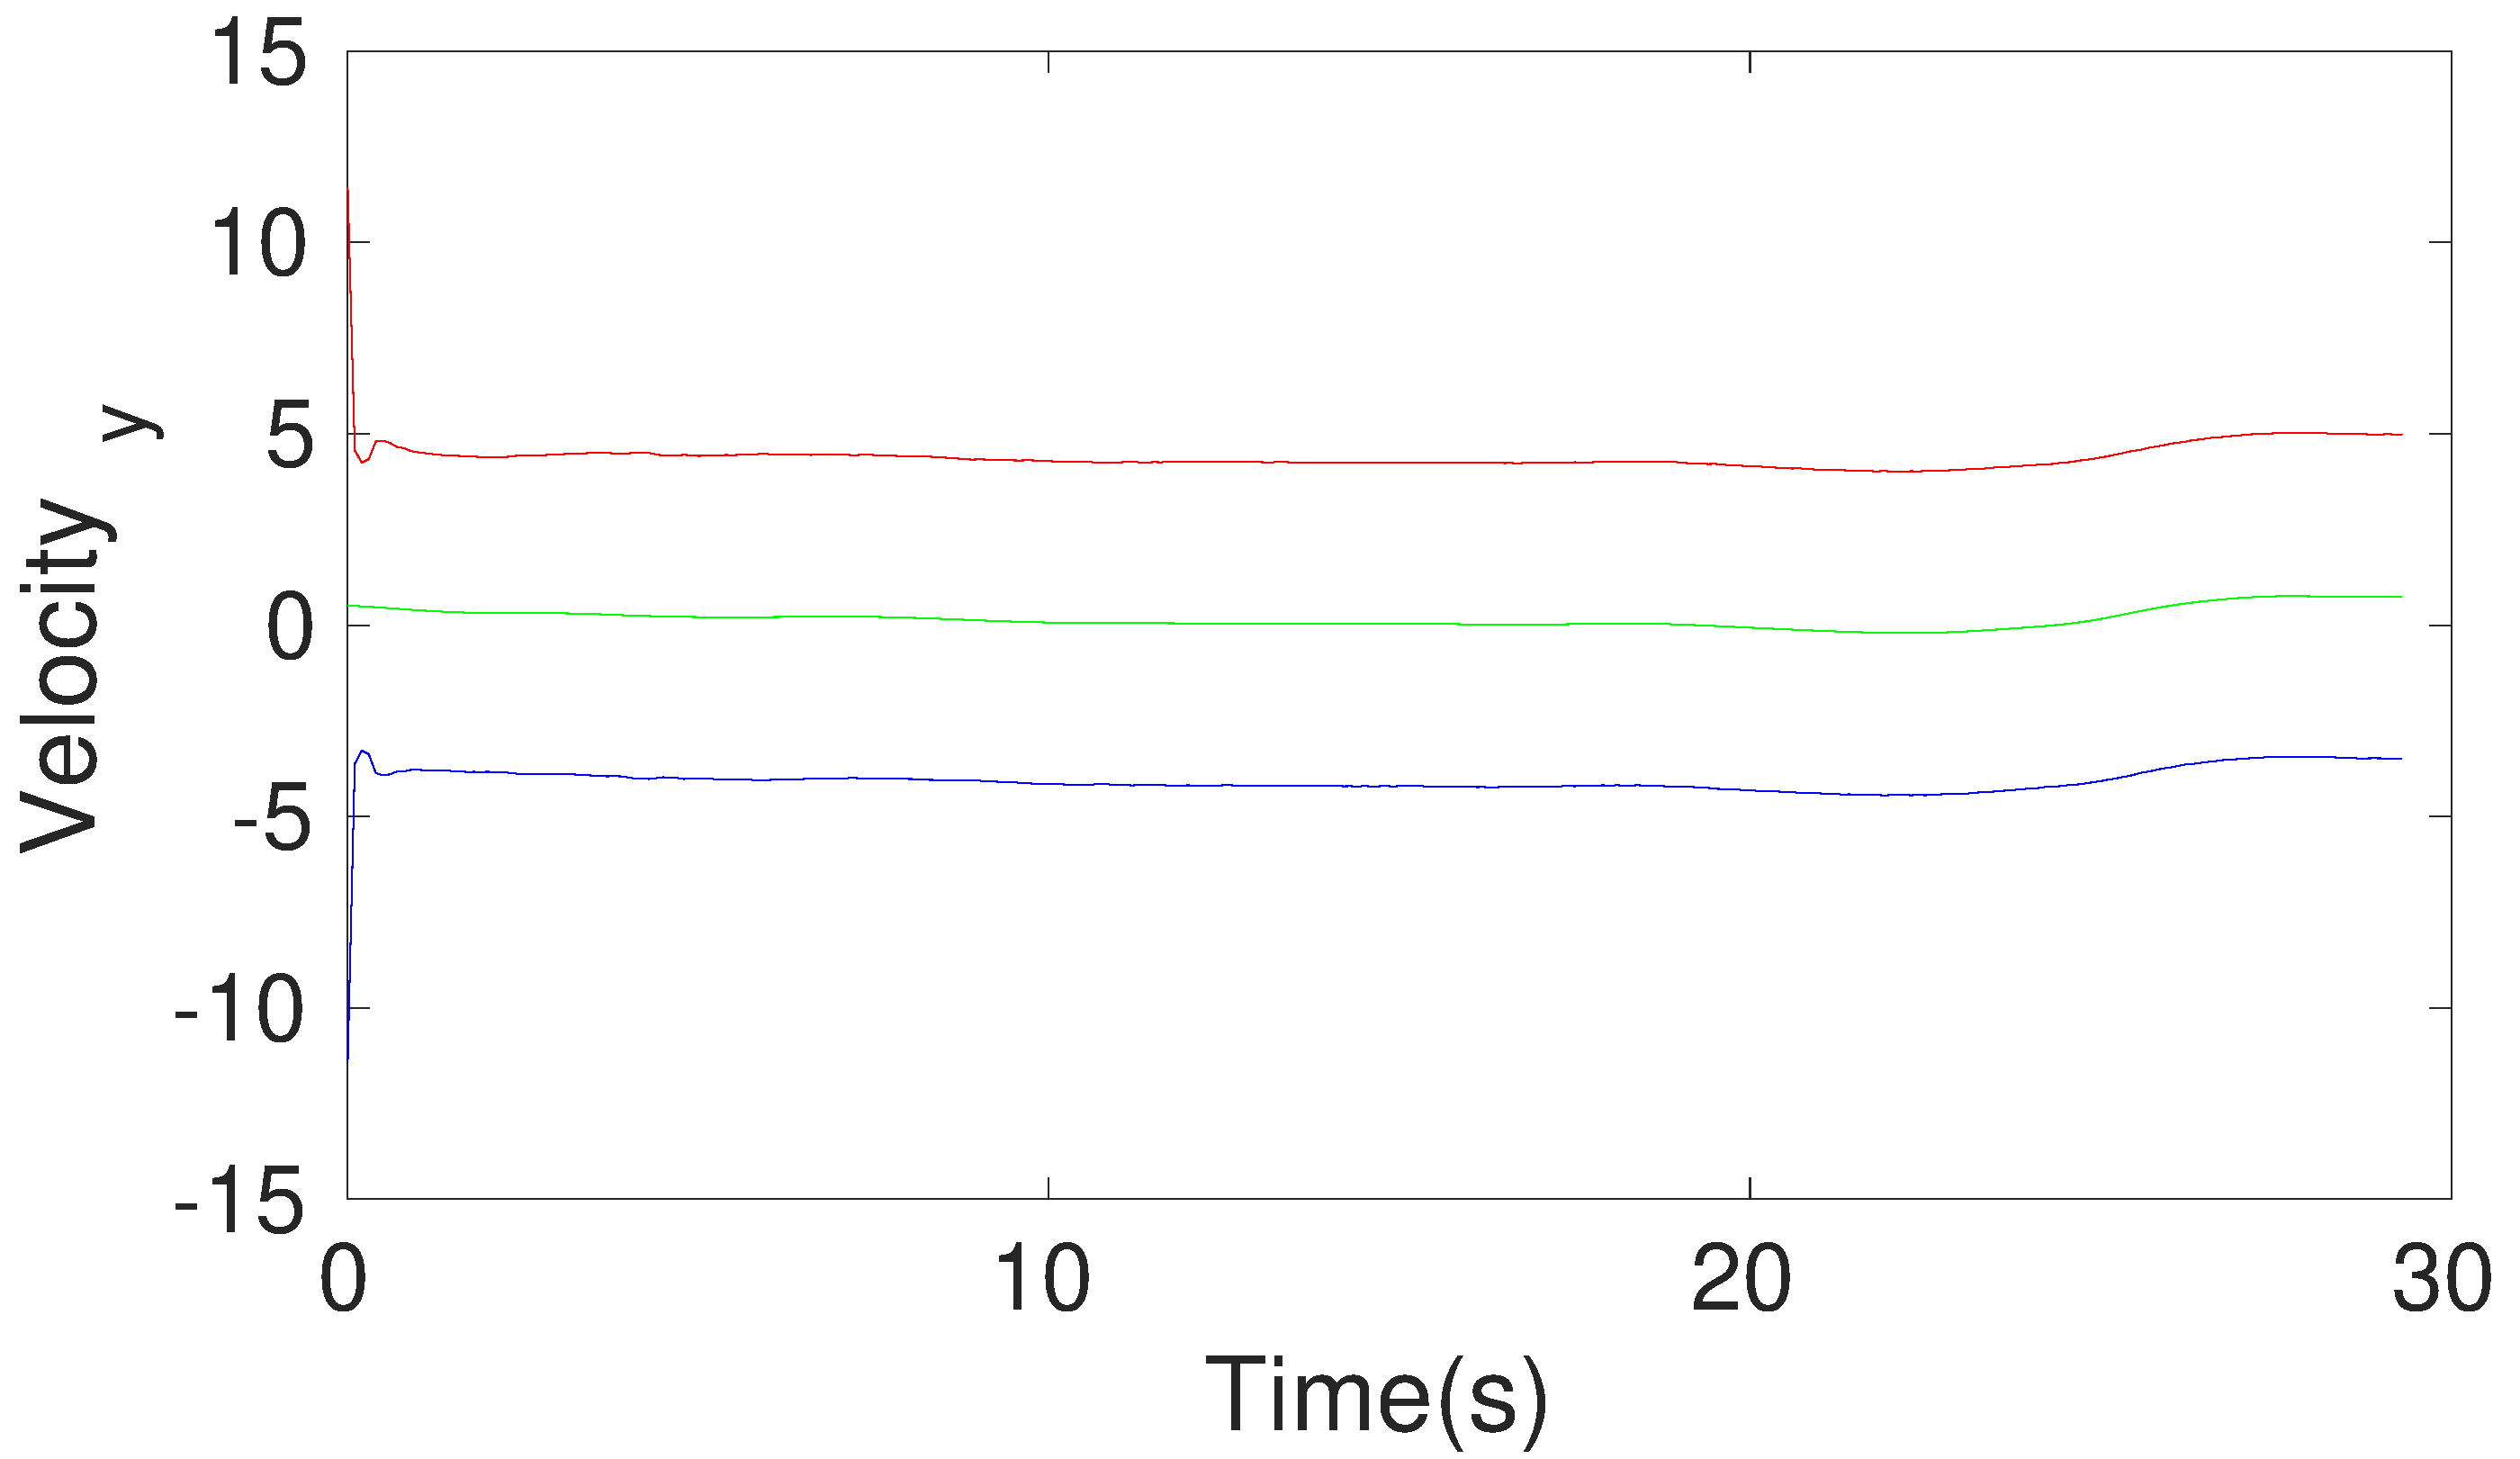
\includegraphics[width=\linewidth]{figures/Frad/s3caSMVelocity_y}
\end{subfigure}
\begin{subfigure}{.5\linewidth}
\centering
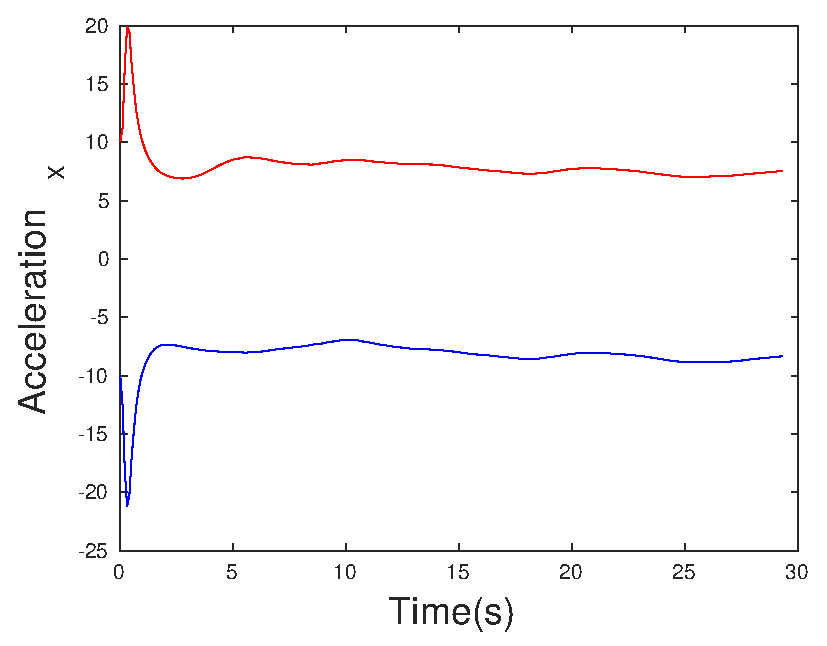
\includegraphics[width=\linewidth]{figures/Frad/s3caSMAcceleration_x}
\end{subfigure}
\begin{subfigure}{.5\linewidth}
\centering
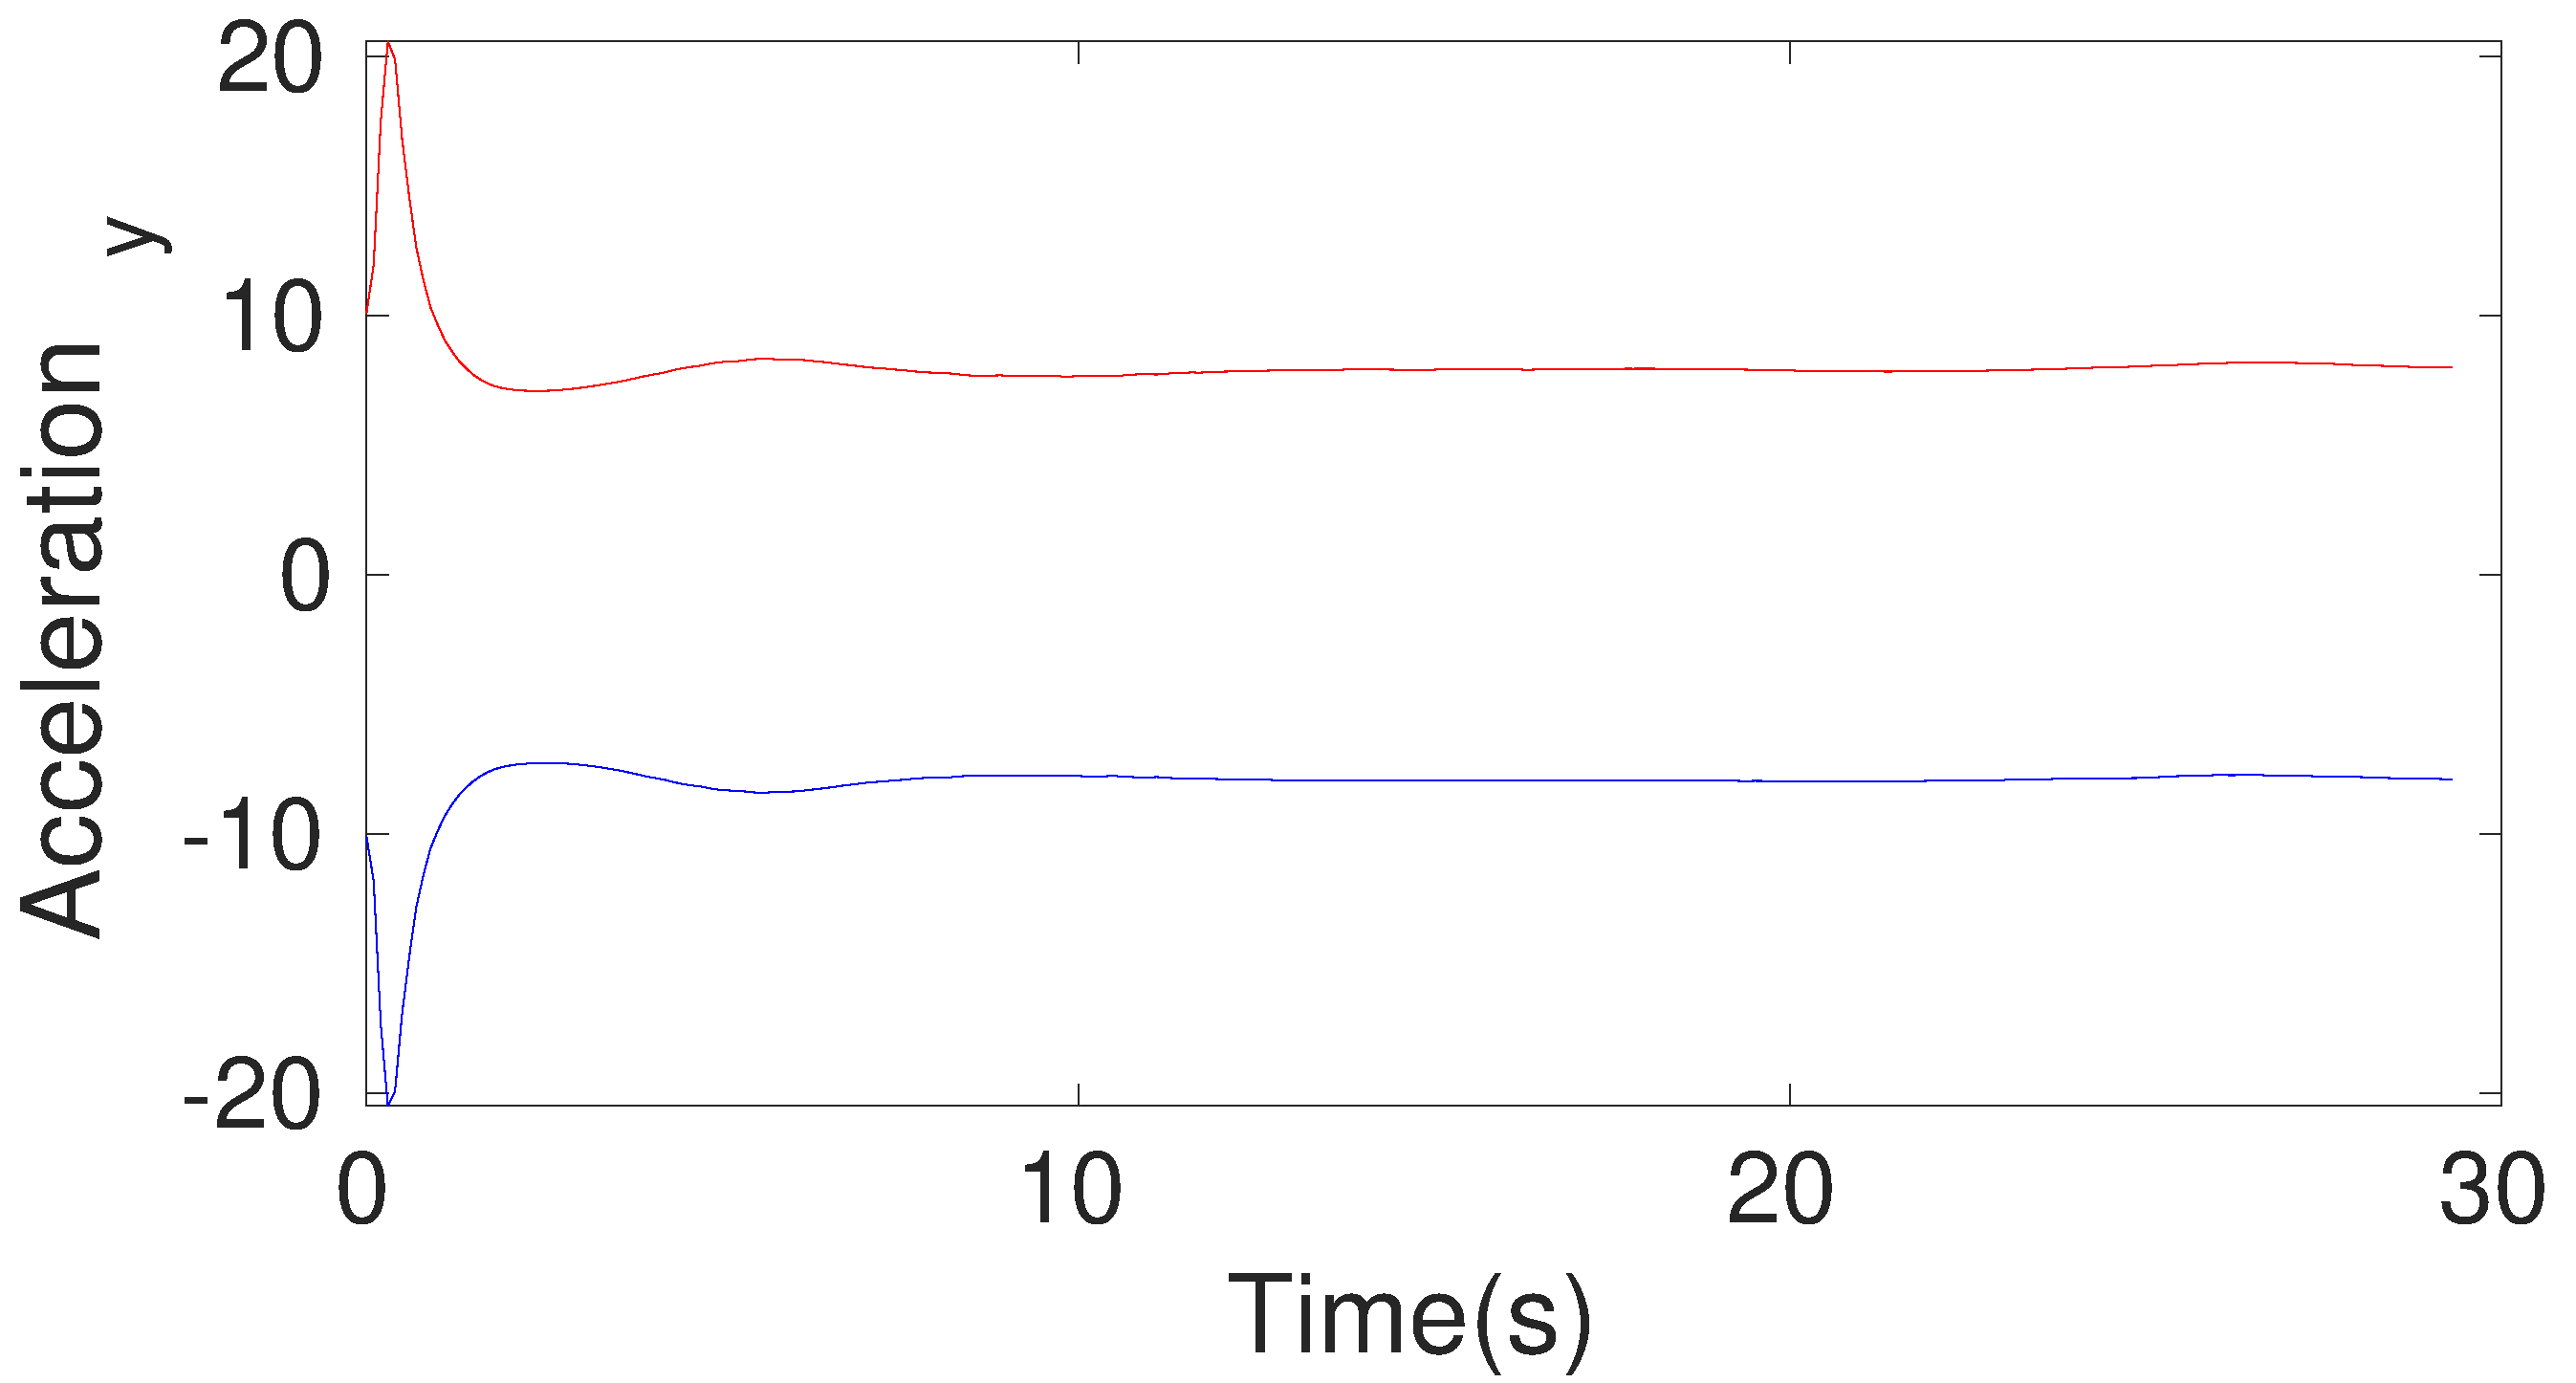
\includegraphics[width=\linewidth]{figures/Frad/s3caSMAcceleration_y}
\end{subfigure}
\caption{Estimation using the F-radius and the constant acceleration model}
\end{figure}

\begin{figure}[h]
\hspace*{\fill} 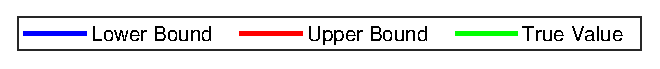
\includegraphics[scale=0.8]{figures/legend}\\\\
\begin{subfigure}{.5\linewidth}
\centering
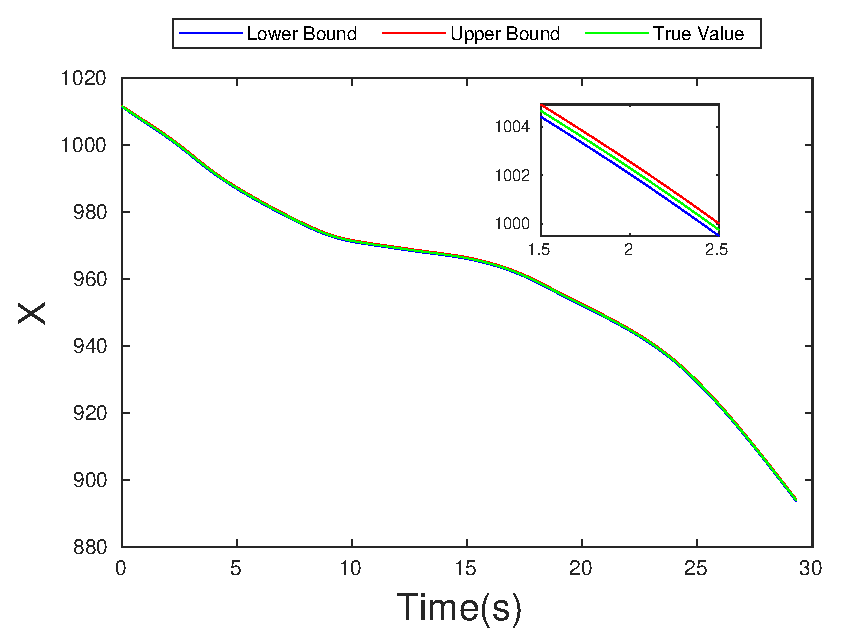
\includegraphics[width=\linewidth]{figures/Frad/s3pmSMX}
\end{subfigure}
\begin{subfigure}{.5\linewidth}
\centering
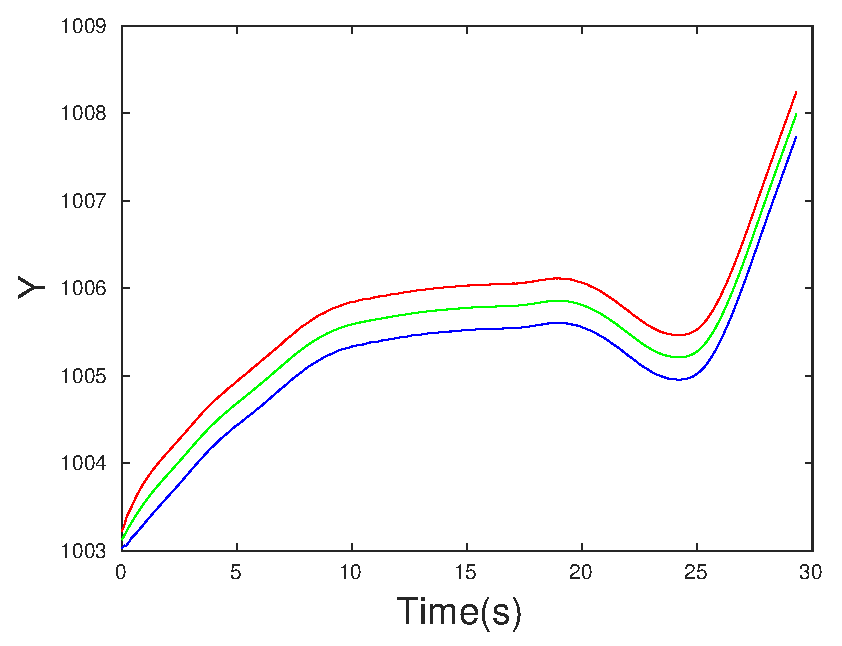
\includegraphics[width=\linewidth]{figures/Frad/s3pmSMY}
\end{subfigure}
\begin{subfigure}{.5\linewidth}
\centering
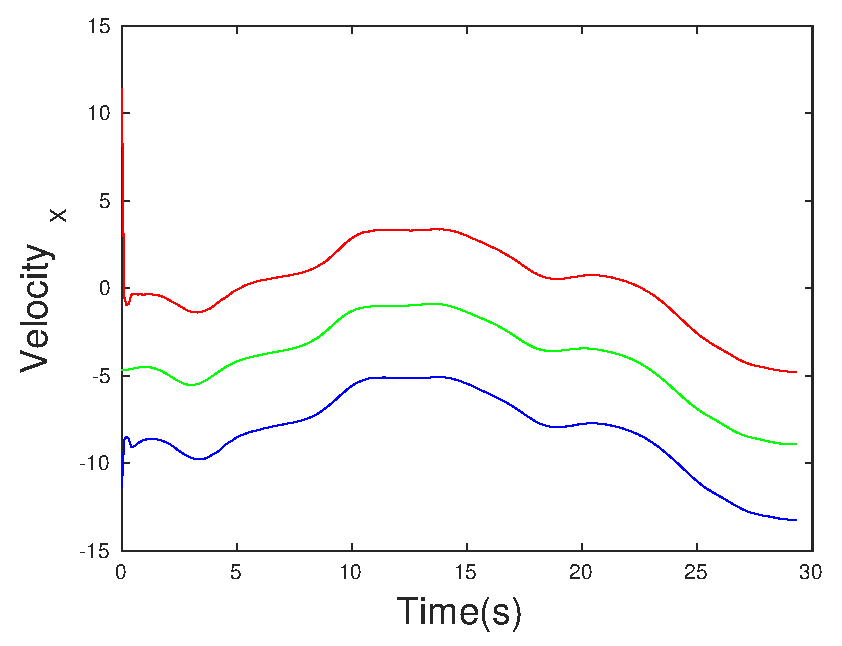
\includegraphics[width=\linewidth]{figures/Frad/s3pmSMVelocity_x}
\end{subfigure}
\begin{subfigure}{.5\linewidth}
\centering
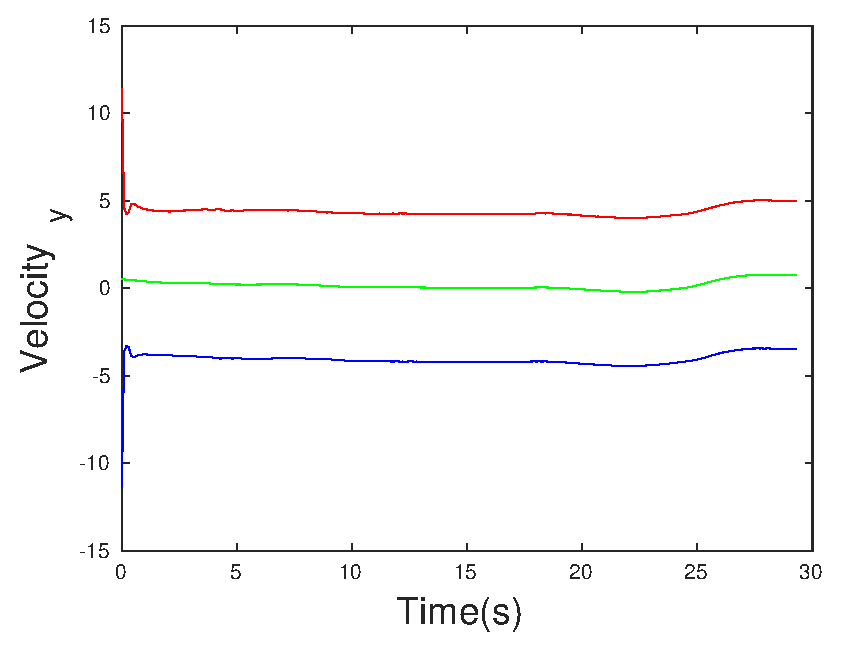
\includegraphics[width=\linewidth]{figures/Frad/s3pmSMVelocity_y}
\end{subfigure}
\begin{subfigure}{.5\linewidth}
\centering
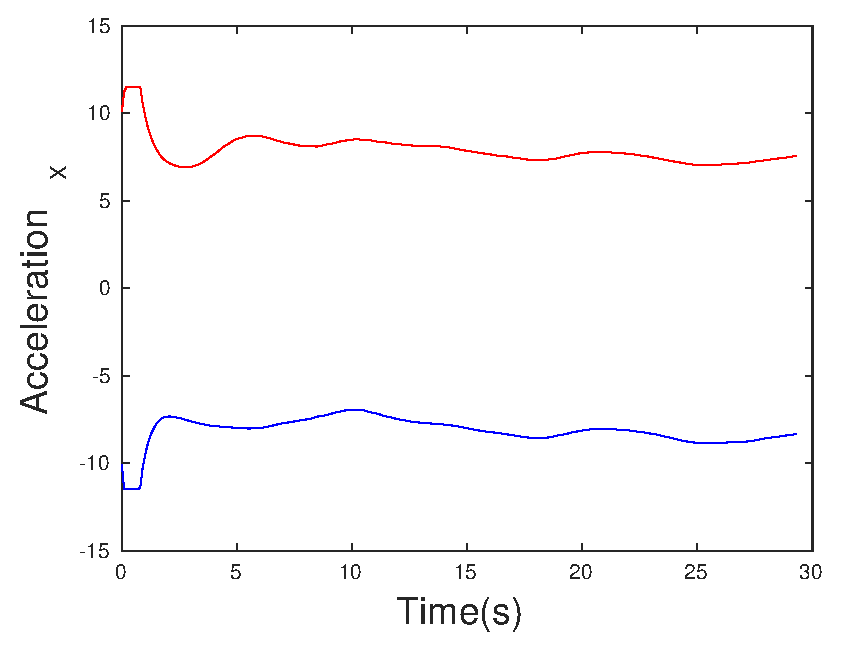
\includegraphics[width=\linewidth]{figures/Frad/s3pmSMAcceleration_x}
\end{subfigure}
\begin{subfigure}{.5\linewidth}
\centering
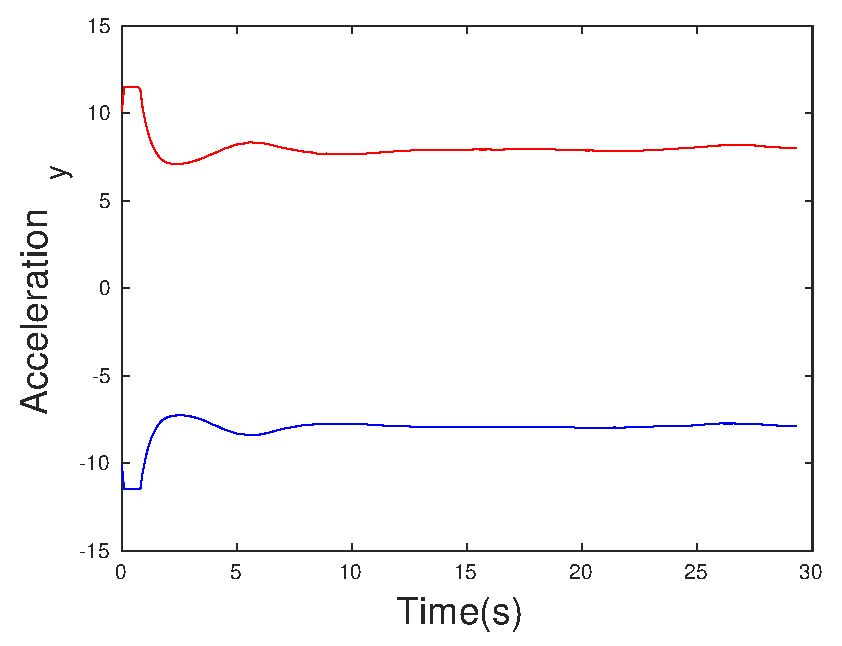
\includegraphics[width=\linewidth]{figures/Frad/s3pmSMAcceleration_y}
\end{subfigure}
\caption{Estimation using the F-radius and the point-mass model}
\end{figure}

\clearpage
\subsection{Segment Minimization using P-Radius}
\FloatBarrier
\begin{figure}[h]
\hspace*{\fill} 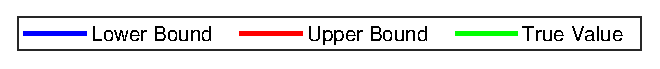
\includegraphics[scale=0.8]{figures/legend}\\\\
\begin{subfigure}{.5\linewidth}
\centering
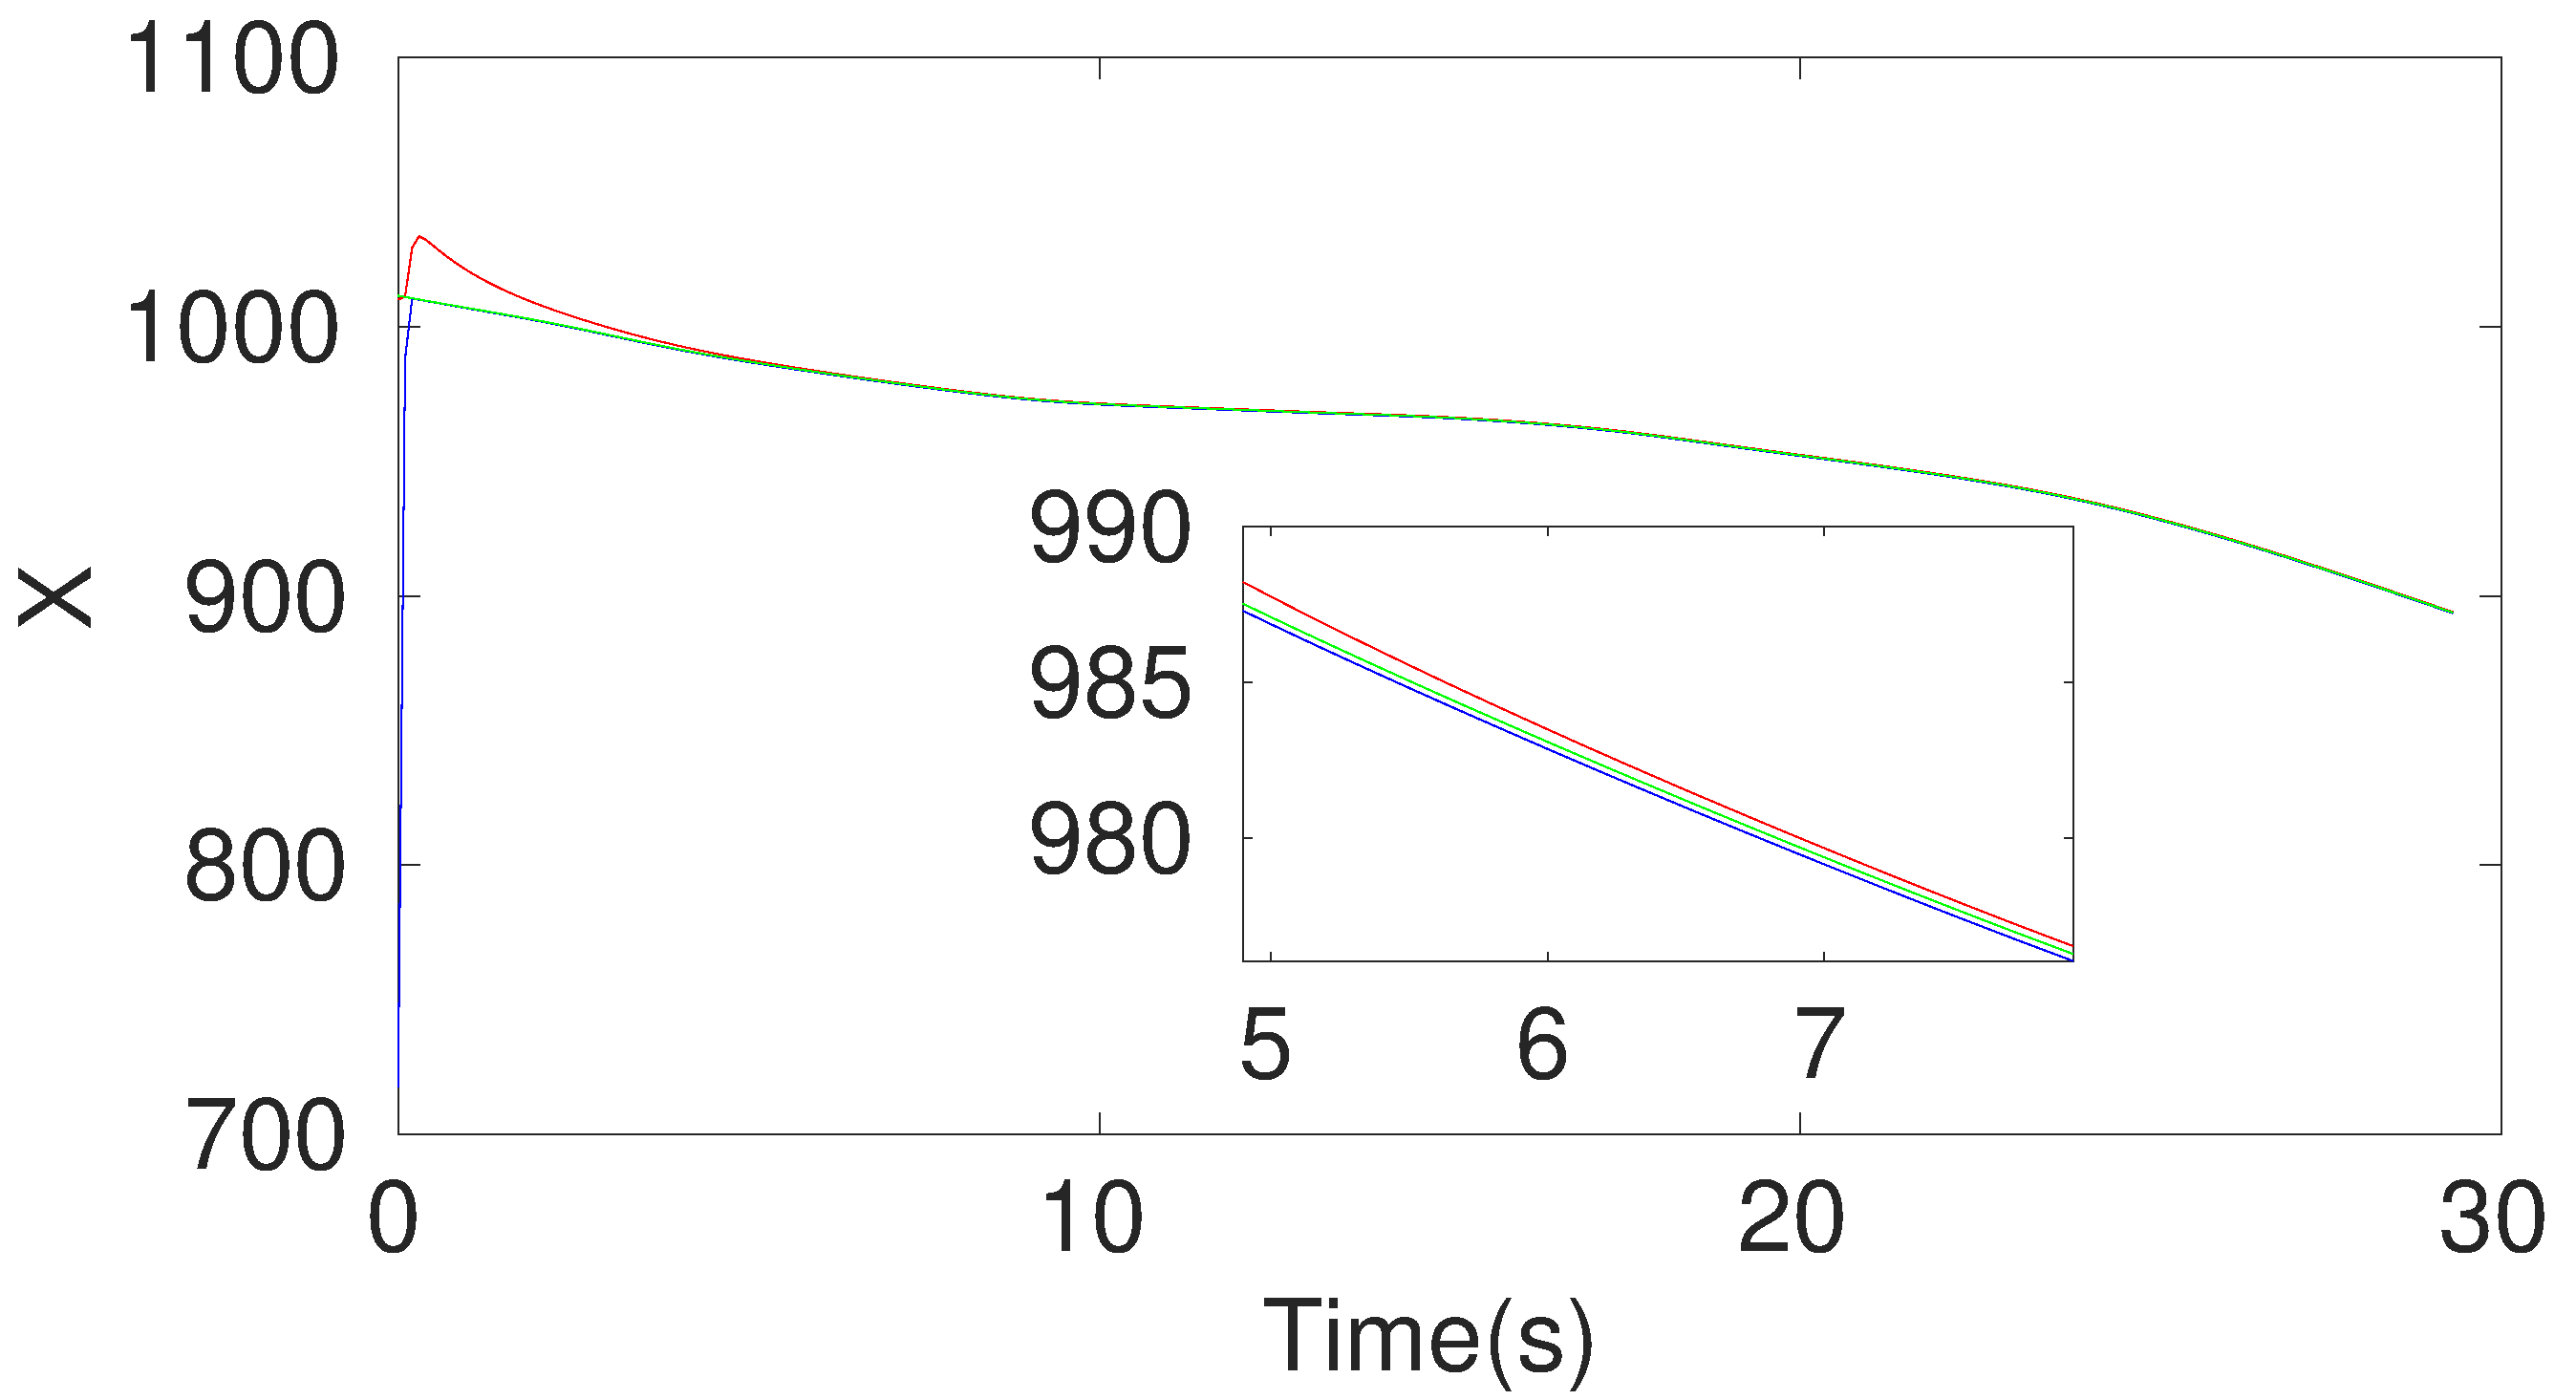
\includegraphics[width=\linewidth]{figures/Prad/s3cvpradX}
\end{subfigure}
\begin{subfigure}{.5\linewidth}
\centering
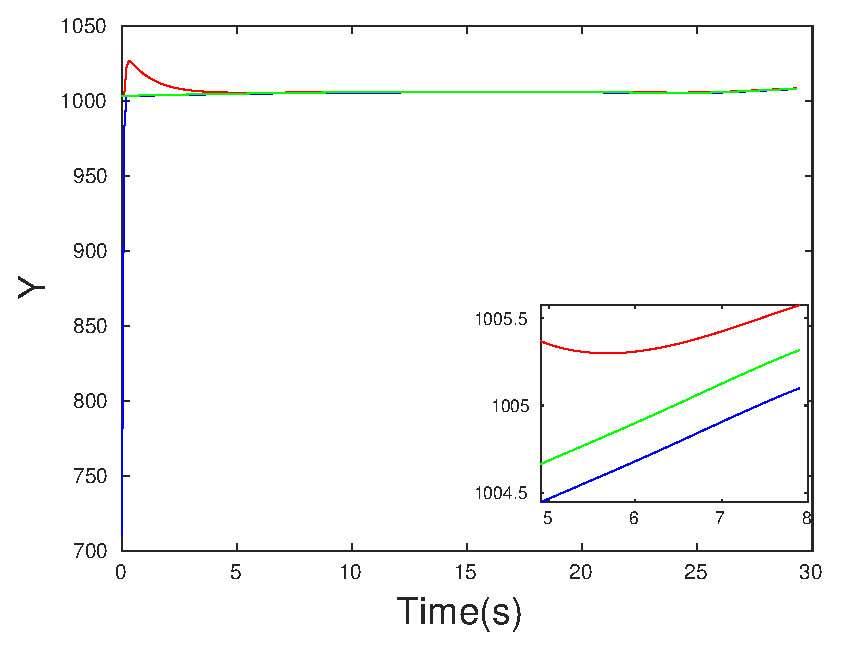
\includegraphics[width=\linewidth]{figures/Prad/s3cvpradY}
\end{subfigure}
\begin{subfigure}{.5\linewidth}
\centering
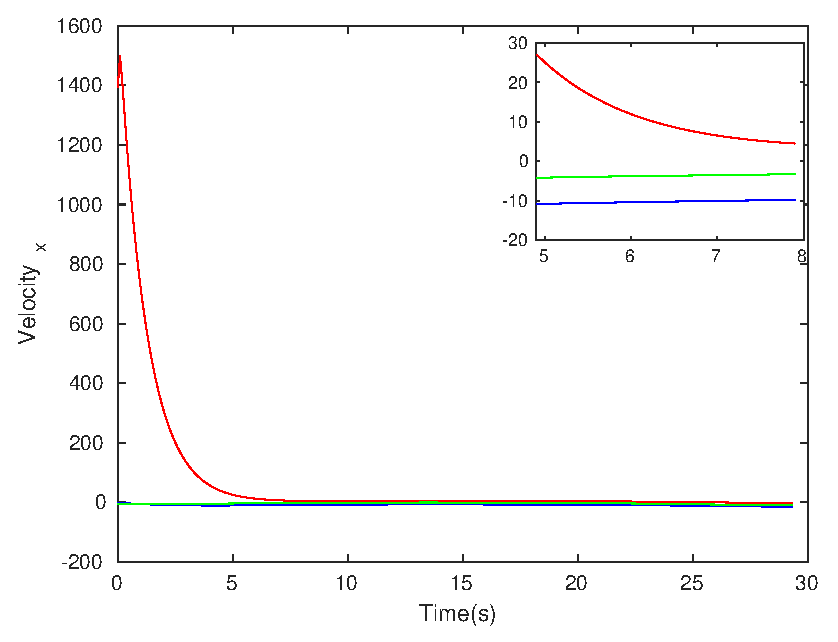
\includegraphics[width=\linewidth]{figures/Prad/s3cvpradVelocity_x}
\end{subfigure}
\begin{subfigure}{.5\linewidth}
\centering
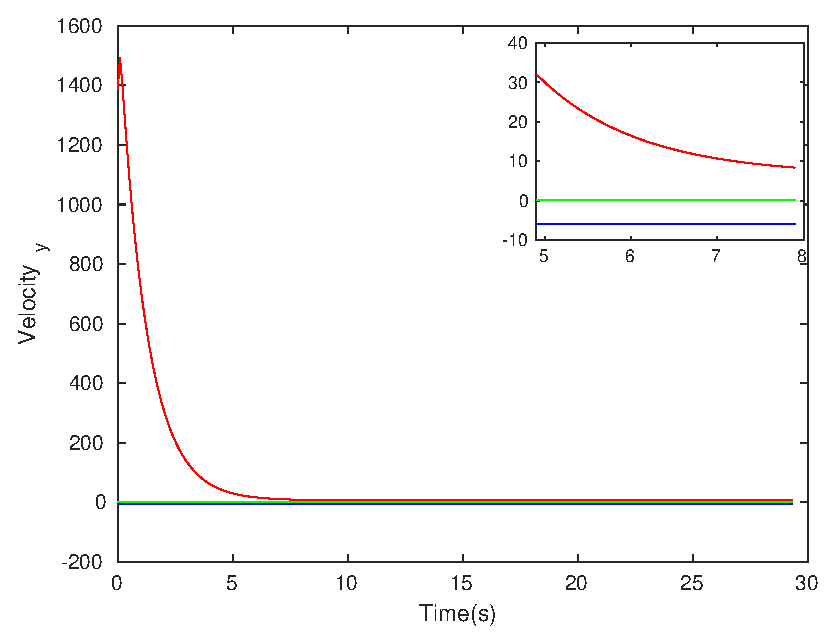
\includegraphics[width=\linewidth]{figures/Prad/s3cvpradVelocity_y}
\end{subfigure}
\caption{Estimation using the P-radius and the constant velocity model}
\end{figure}

\begin{figure}[h]
\hspace*{\fill} 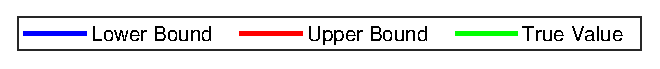
\includegraphics[scale=0.8]{figures/legend}\\\\
\begin{subfigure}{.5\linewidth}
\centering
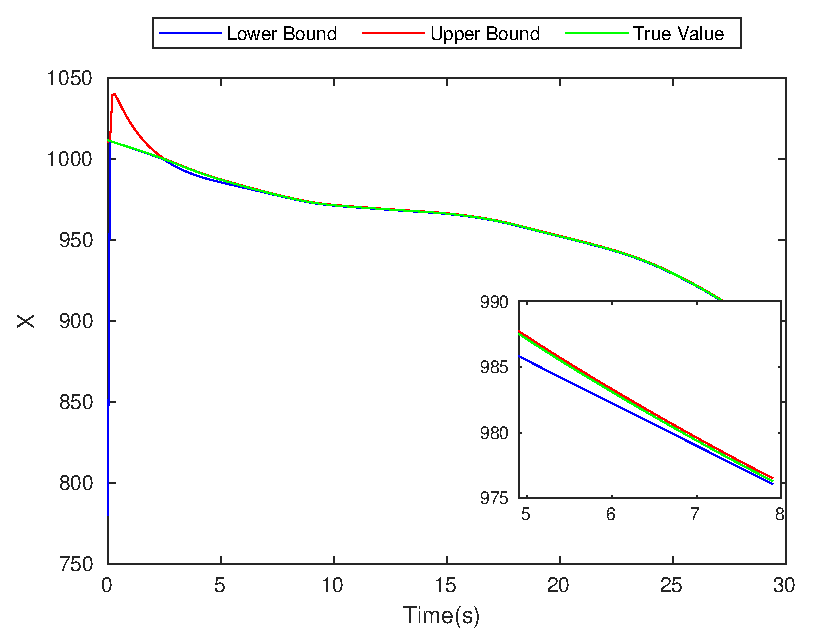
\includegraphics[width=\linewidth]{figures/Prad/s3capradX}
\end{subfigure}
\begin{subfigure}{.5\linewidth}
\centering
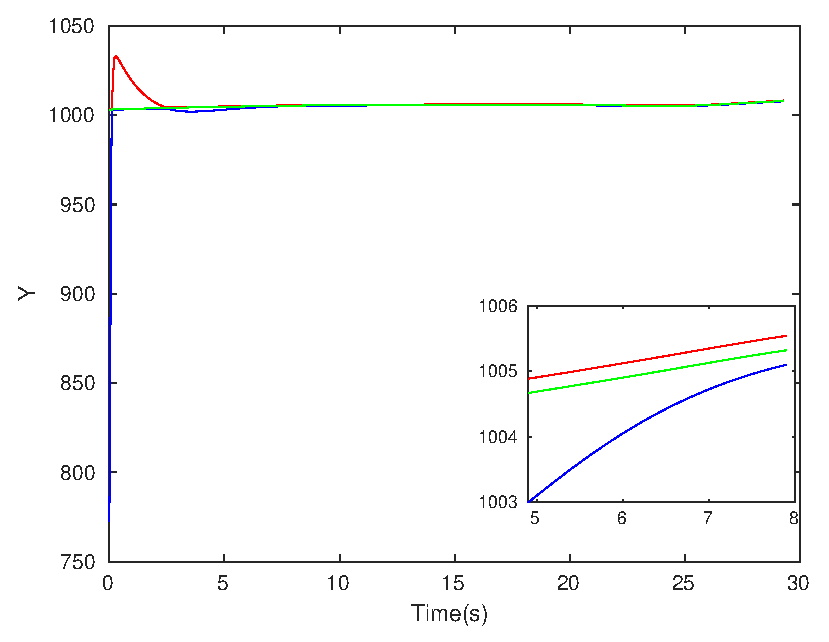
\includegraphics[width=\linewidth]{figures/Prad/s3capradY}
\end{subfigure}
\begin{subfigure}{.5\linewidth}
\centering
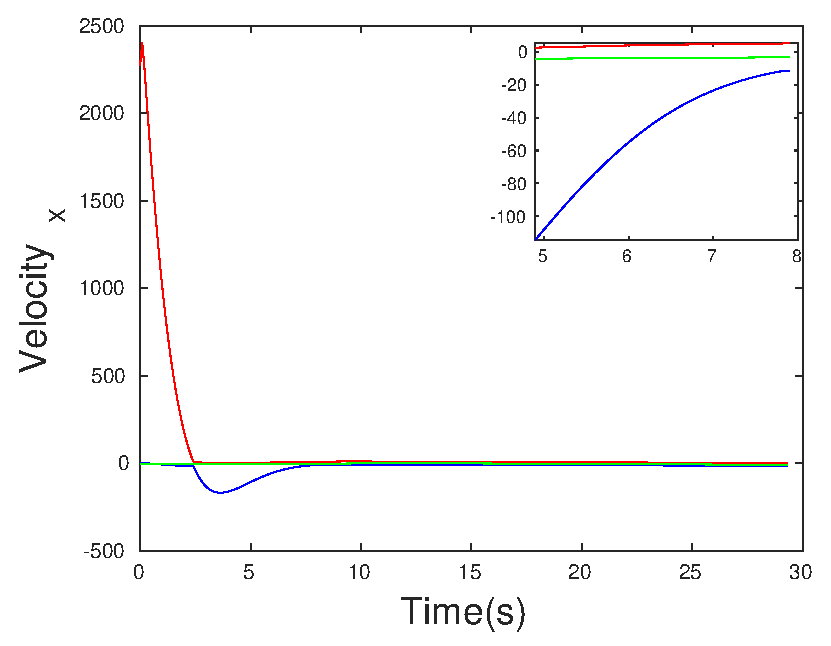
\includegraphics[width=\linewidth]{figures/Prad/s3capradVelocity_x}
\end{subfigure}
\begin{subfigure}{.5\linewidth}
\centering
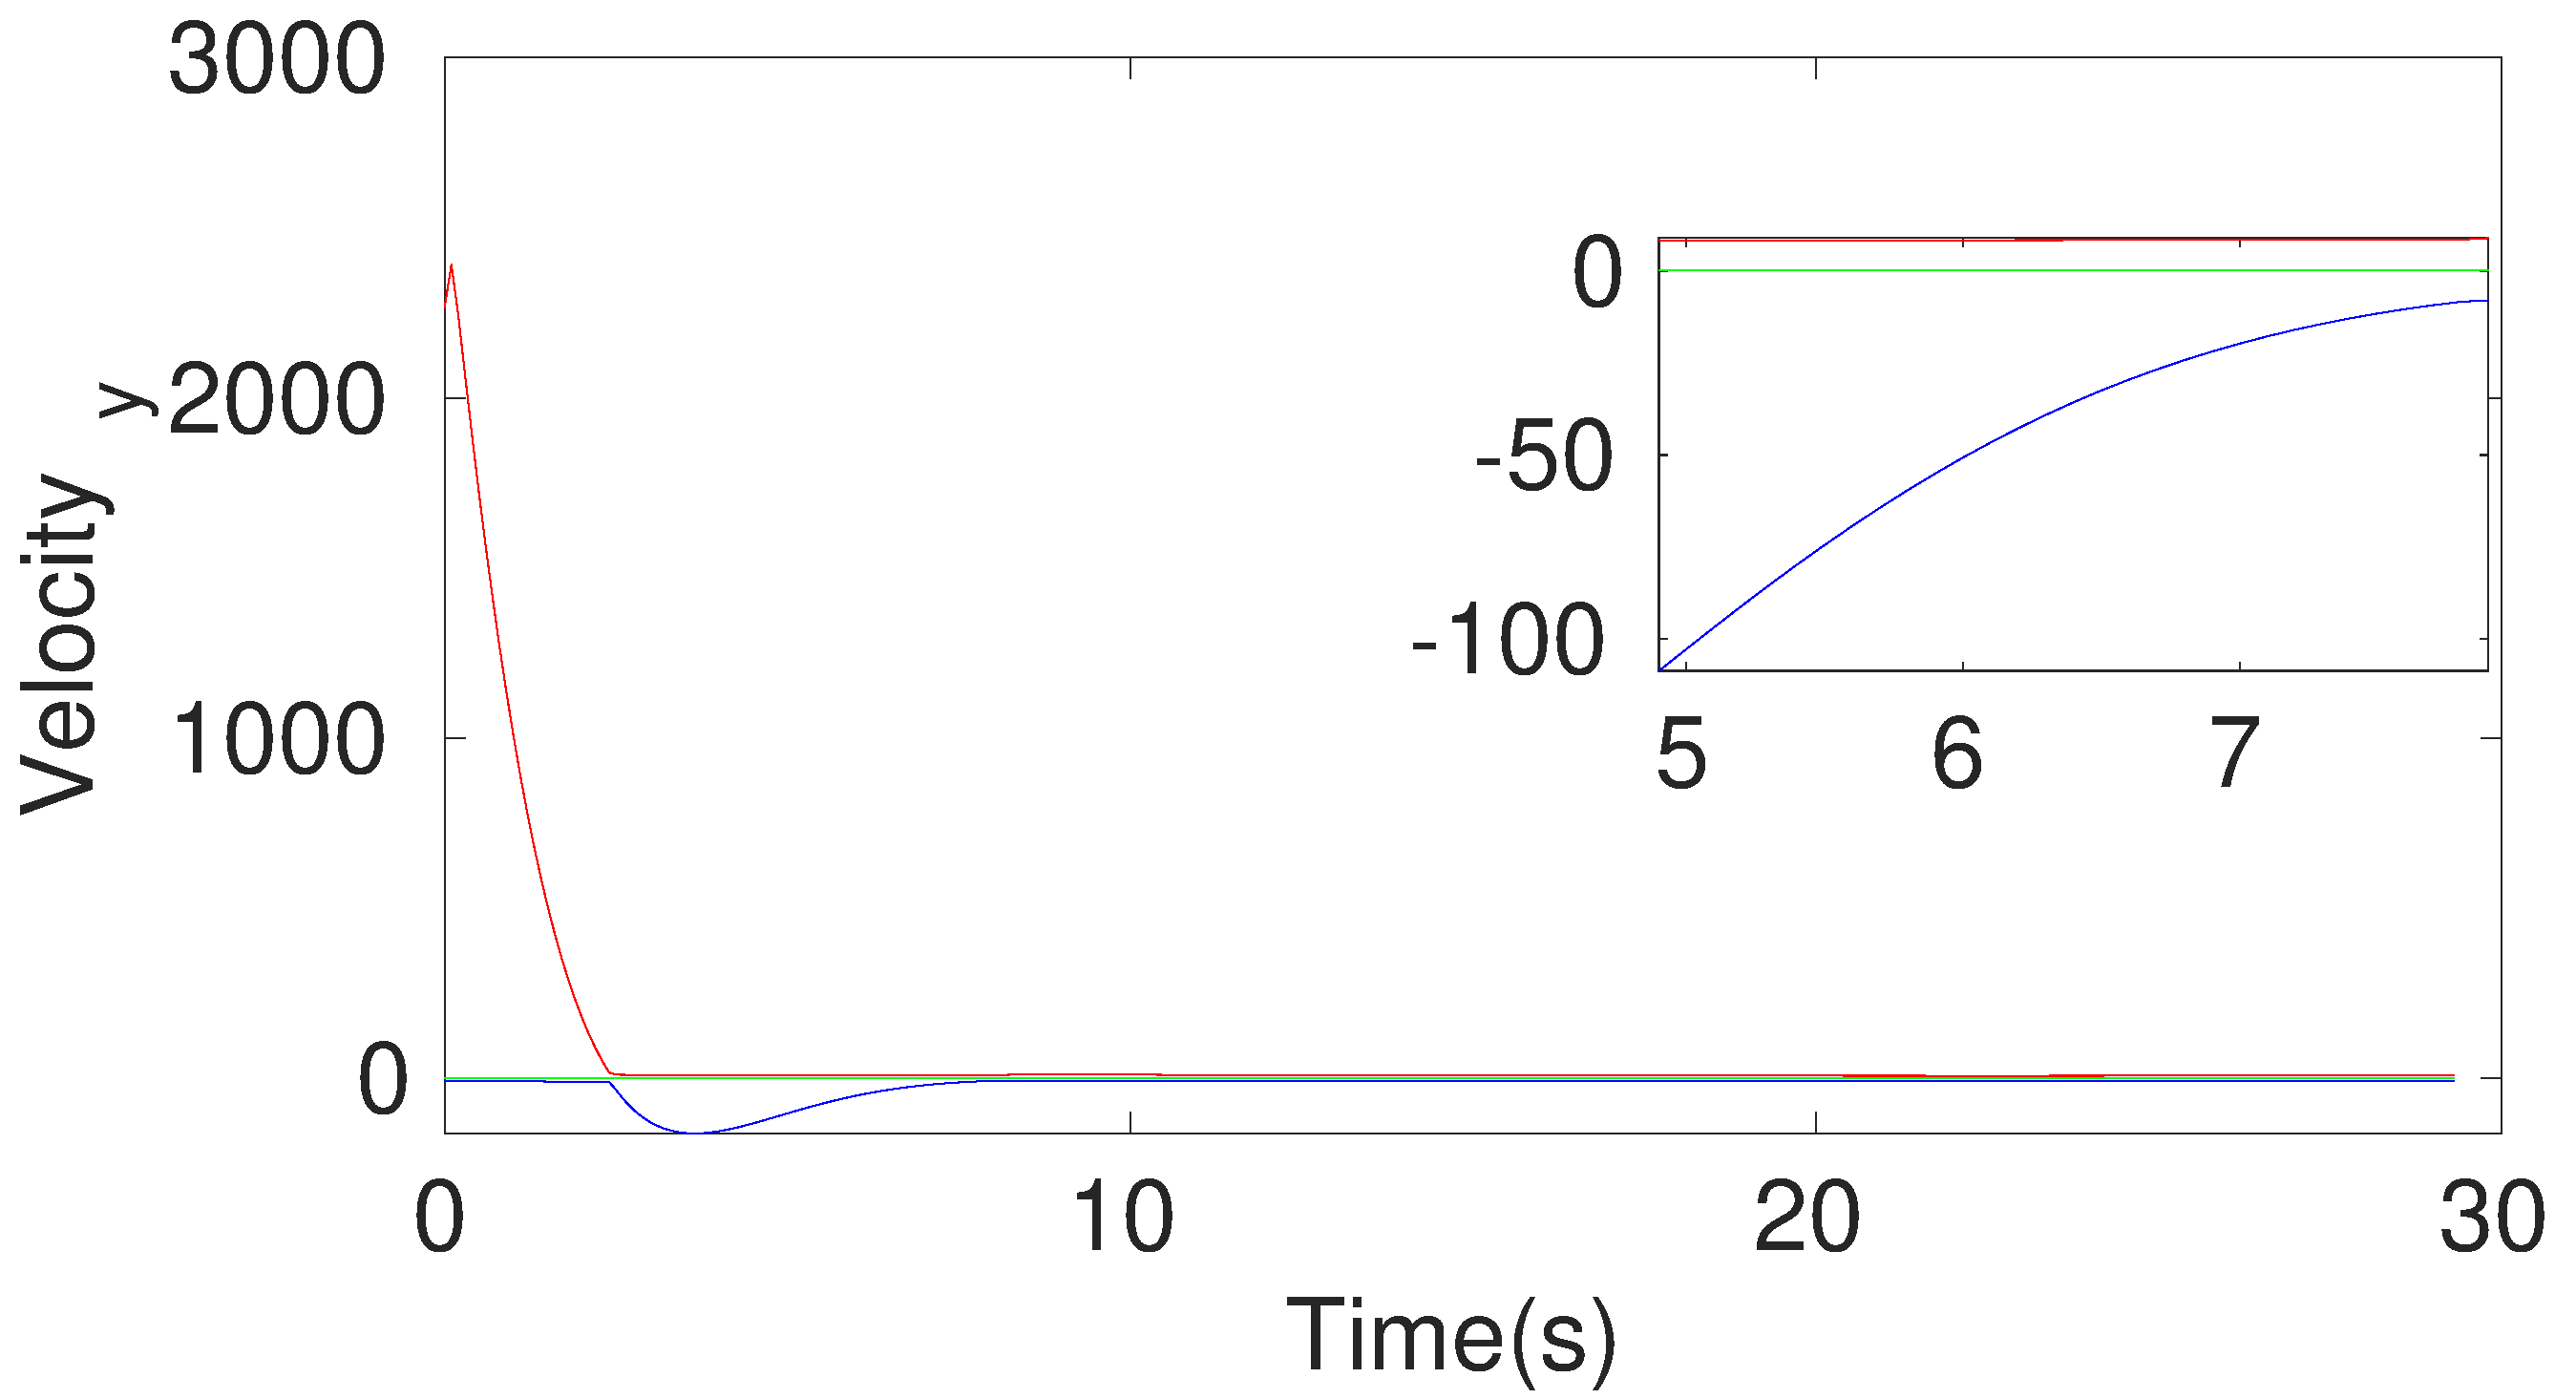
\includegraphics[width=\linewidth]{figures/Prad/s3capradVelocity_y}
\end{subfigure}
\begin{subfigure}{.5\linewidth}
\centering
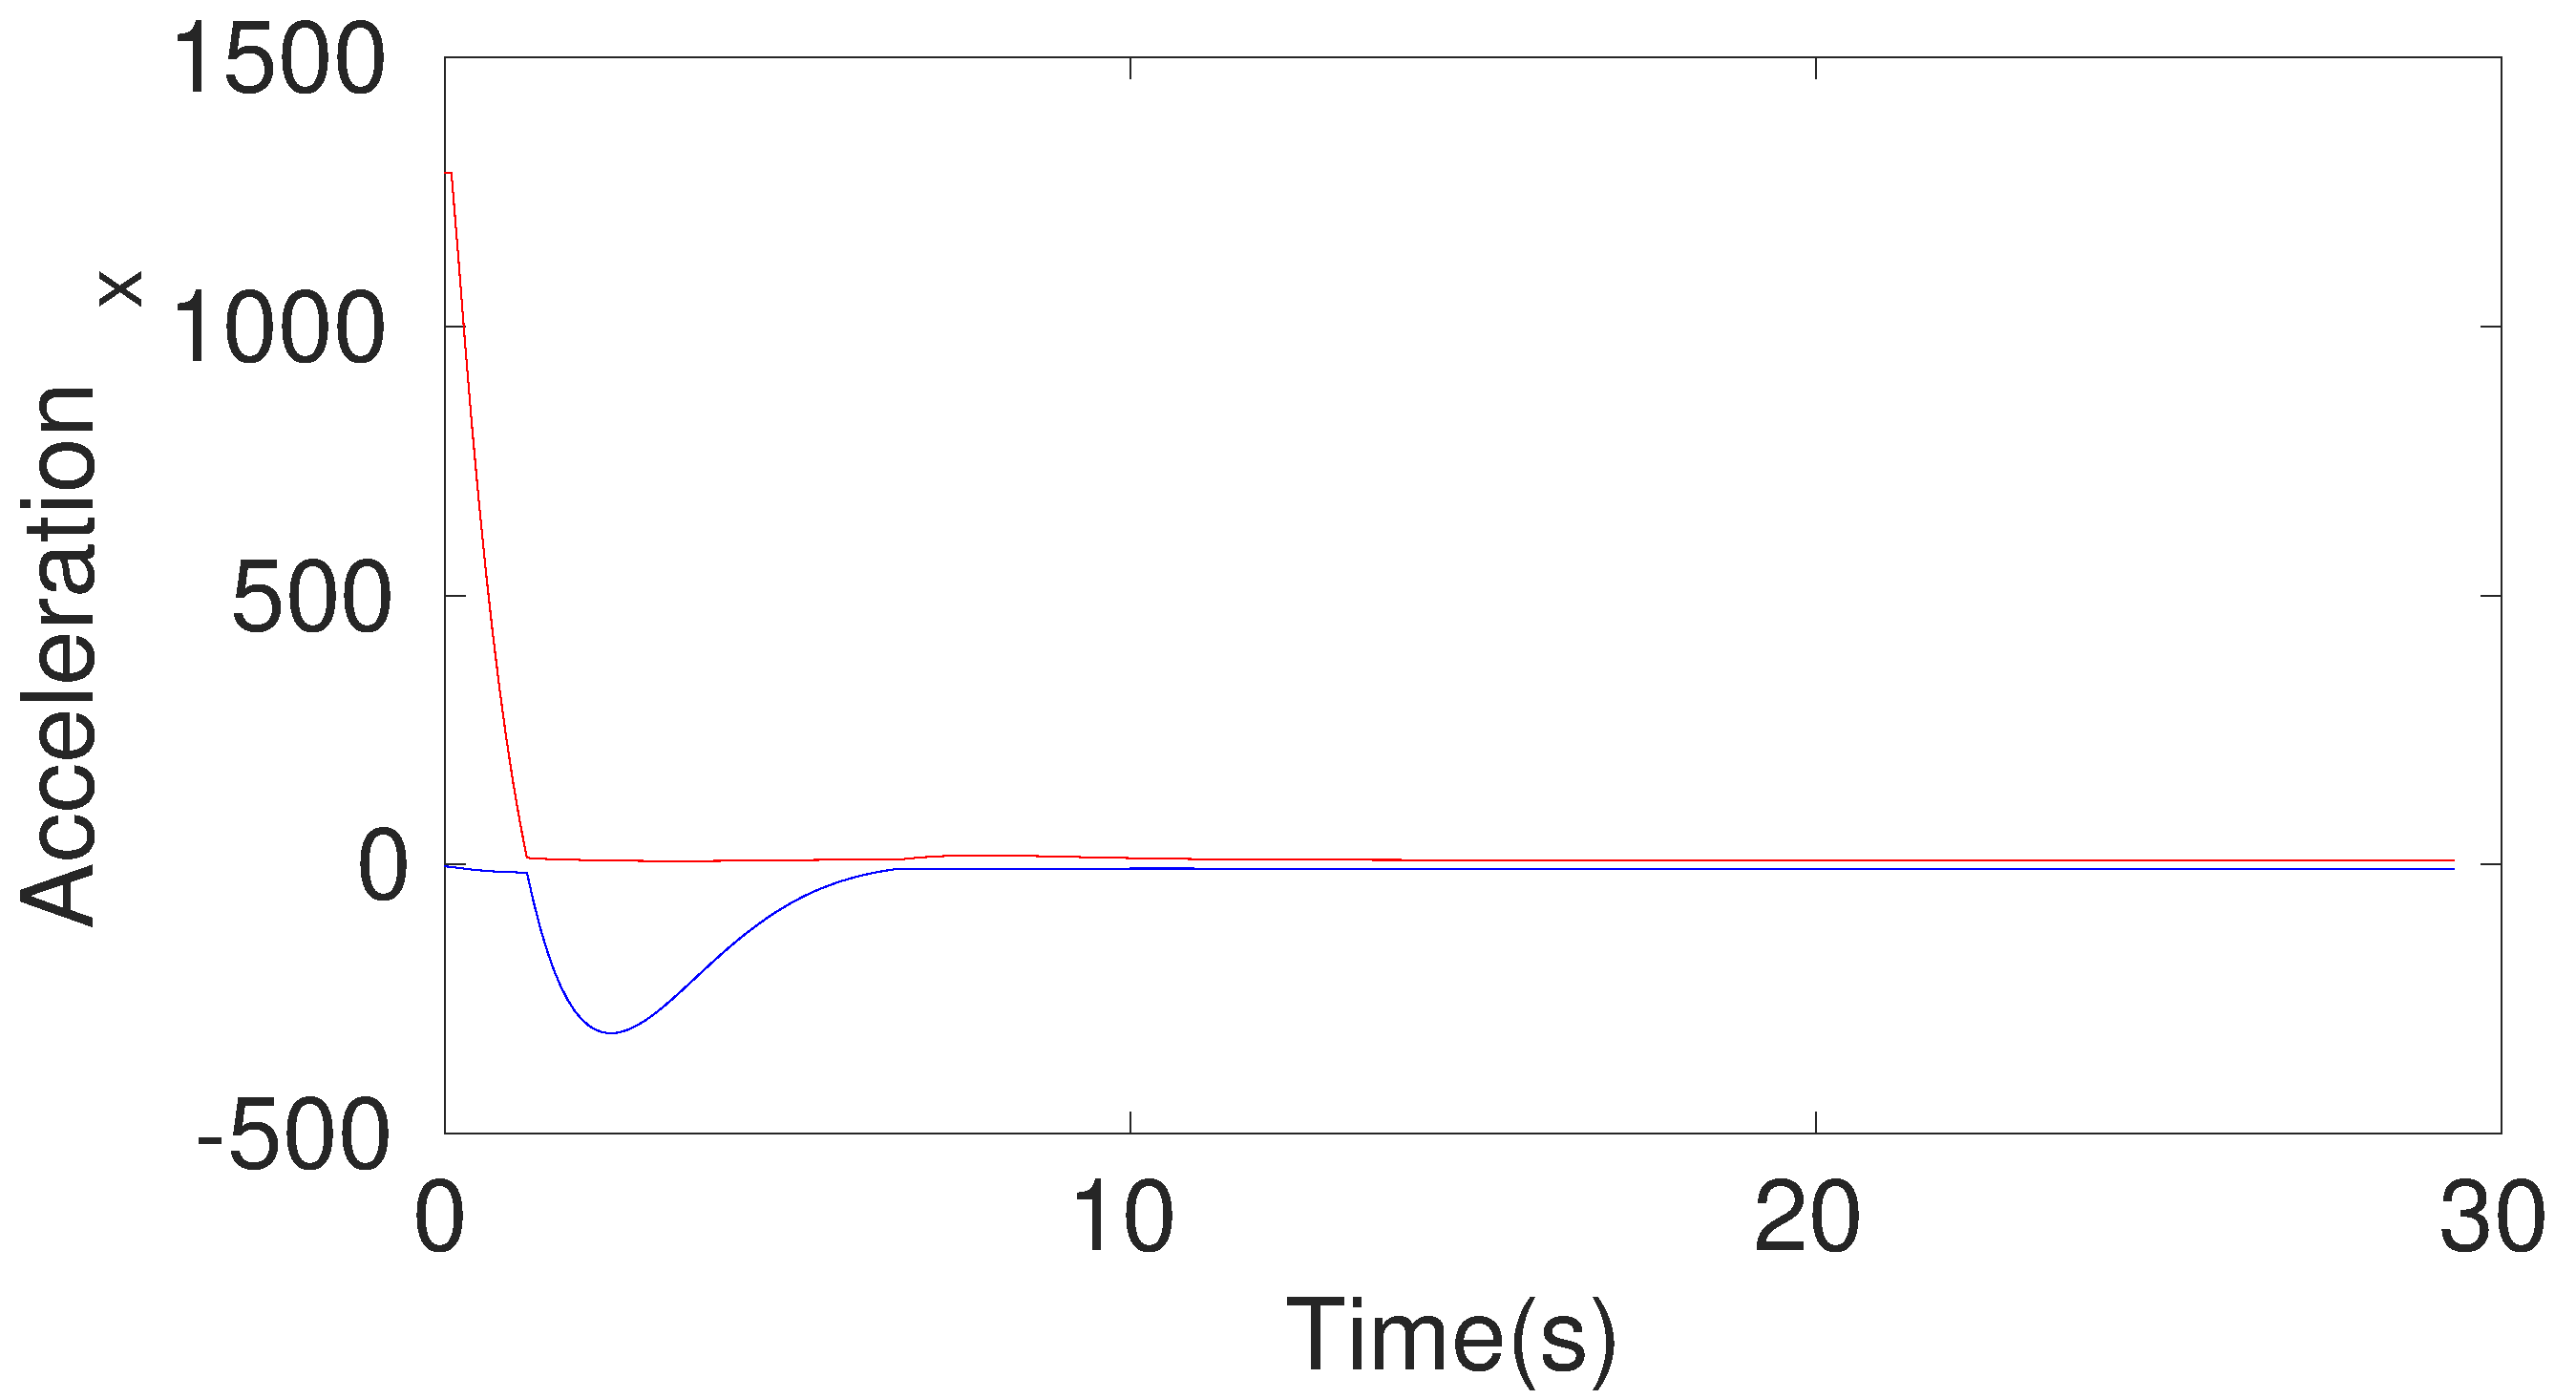
\includegraphics[width=\linewidth]{figures/Prad/s3capradAcceleration_x}
\end{subfigure}
\begin{subfigure}{.5\linewidth}
\centering
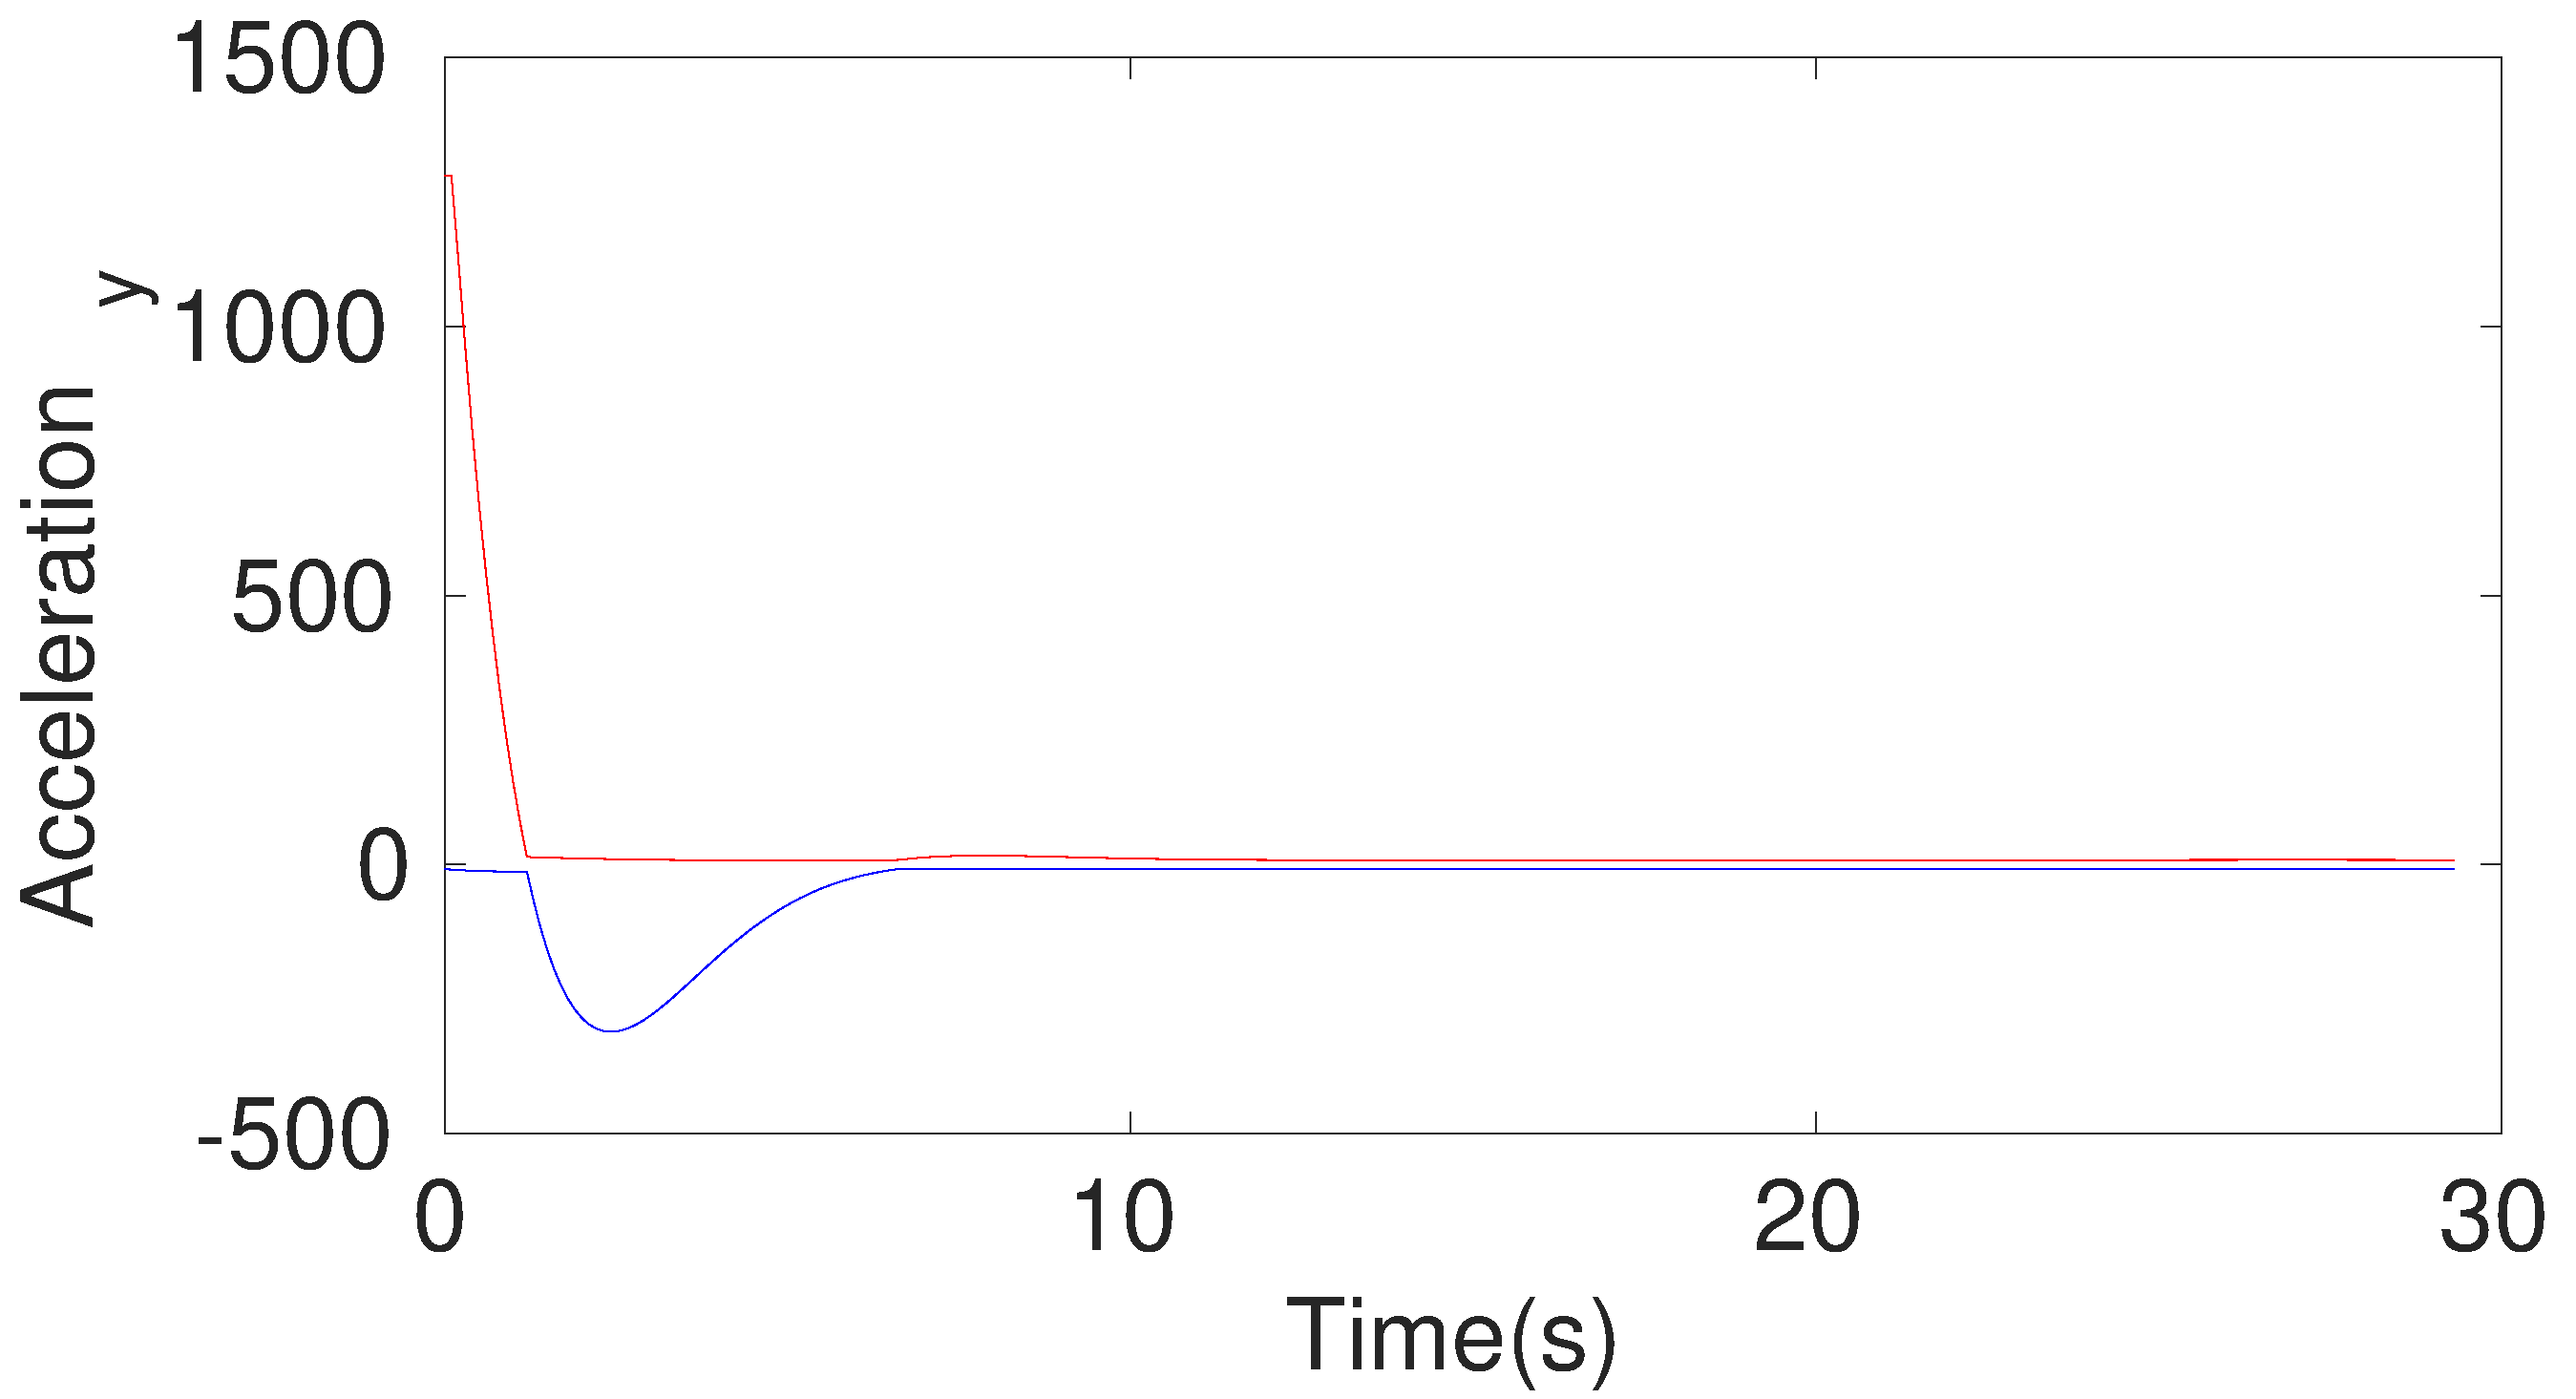
\includegraphics[width=\linewidth]{figures/Prad/s3capradAcceleration_y}
\end{subfigure}
\caption{Estimation using the P-radius and the constant acceleration model}
\end{figure}

\begin{figure}[h]
\hspace*{\fill} 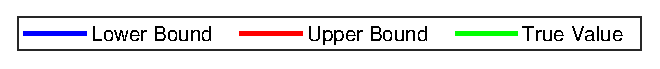
\includegraphics[scale=0.8]{figures/legend}\\\\
\begin{subfigure}{.5\linewidth}
\centering
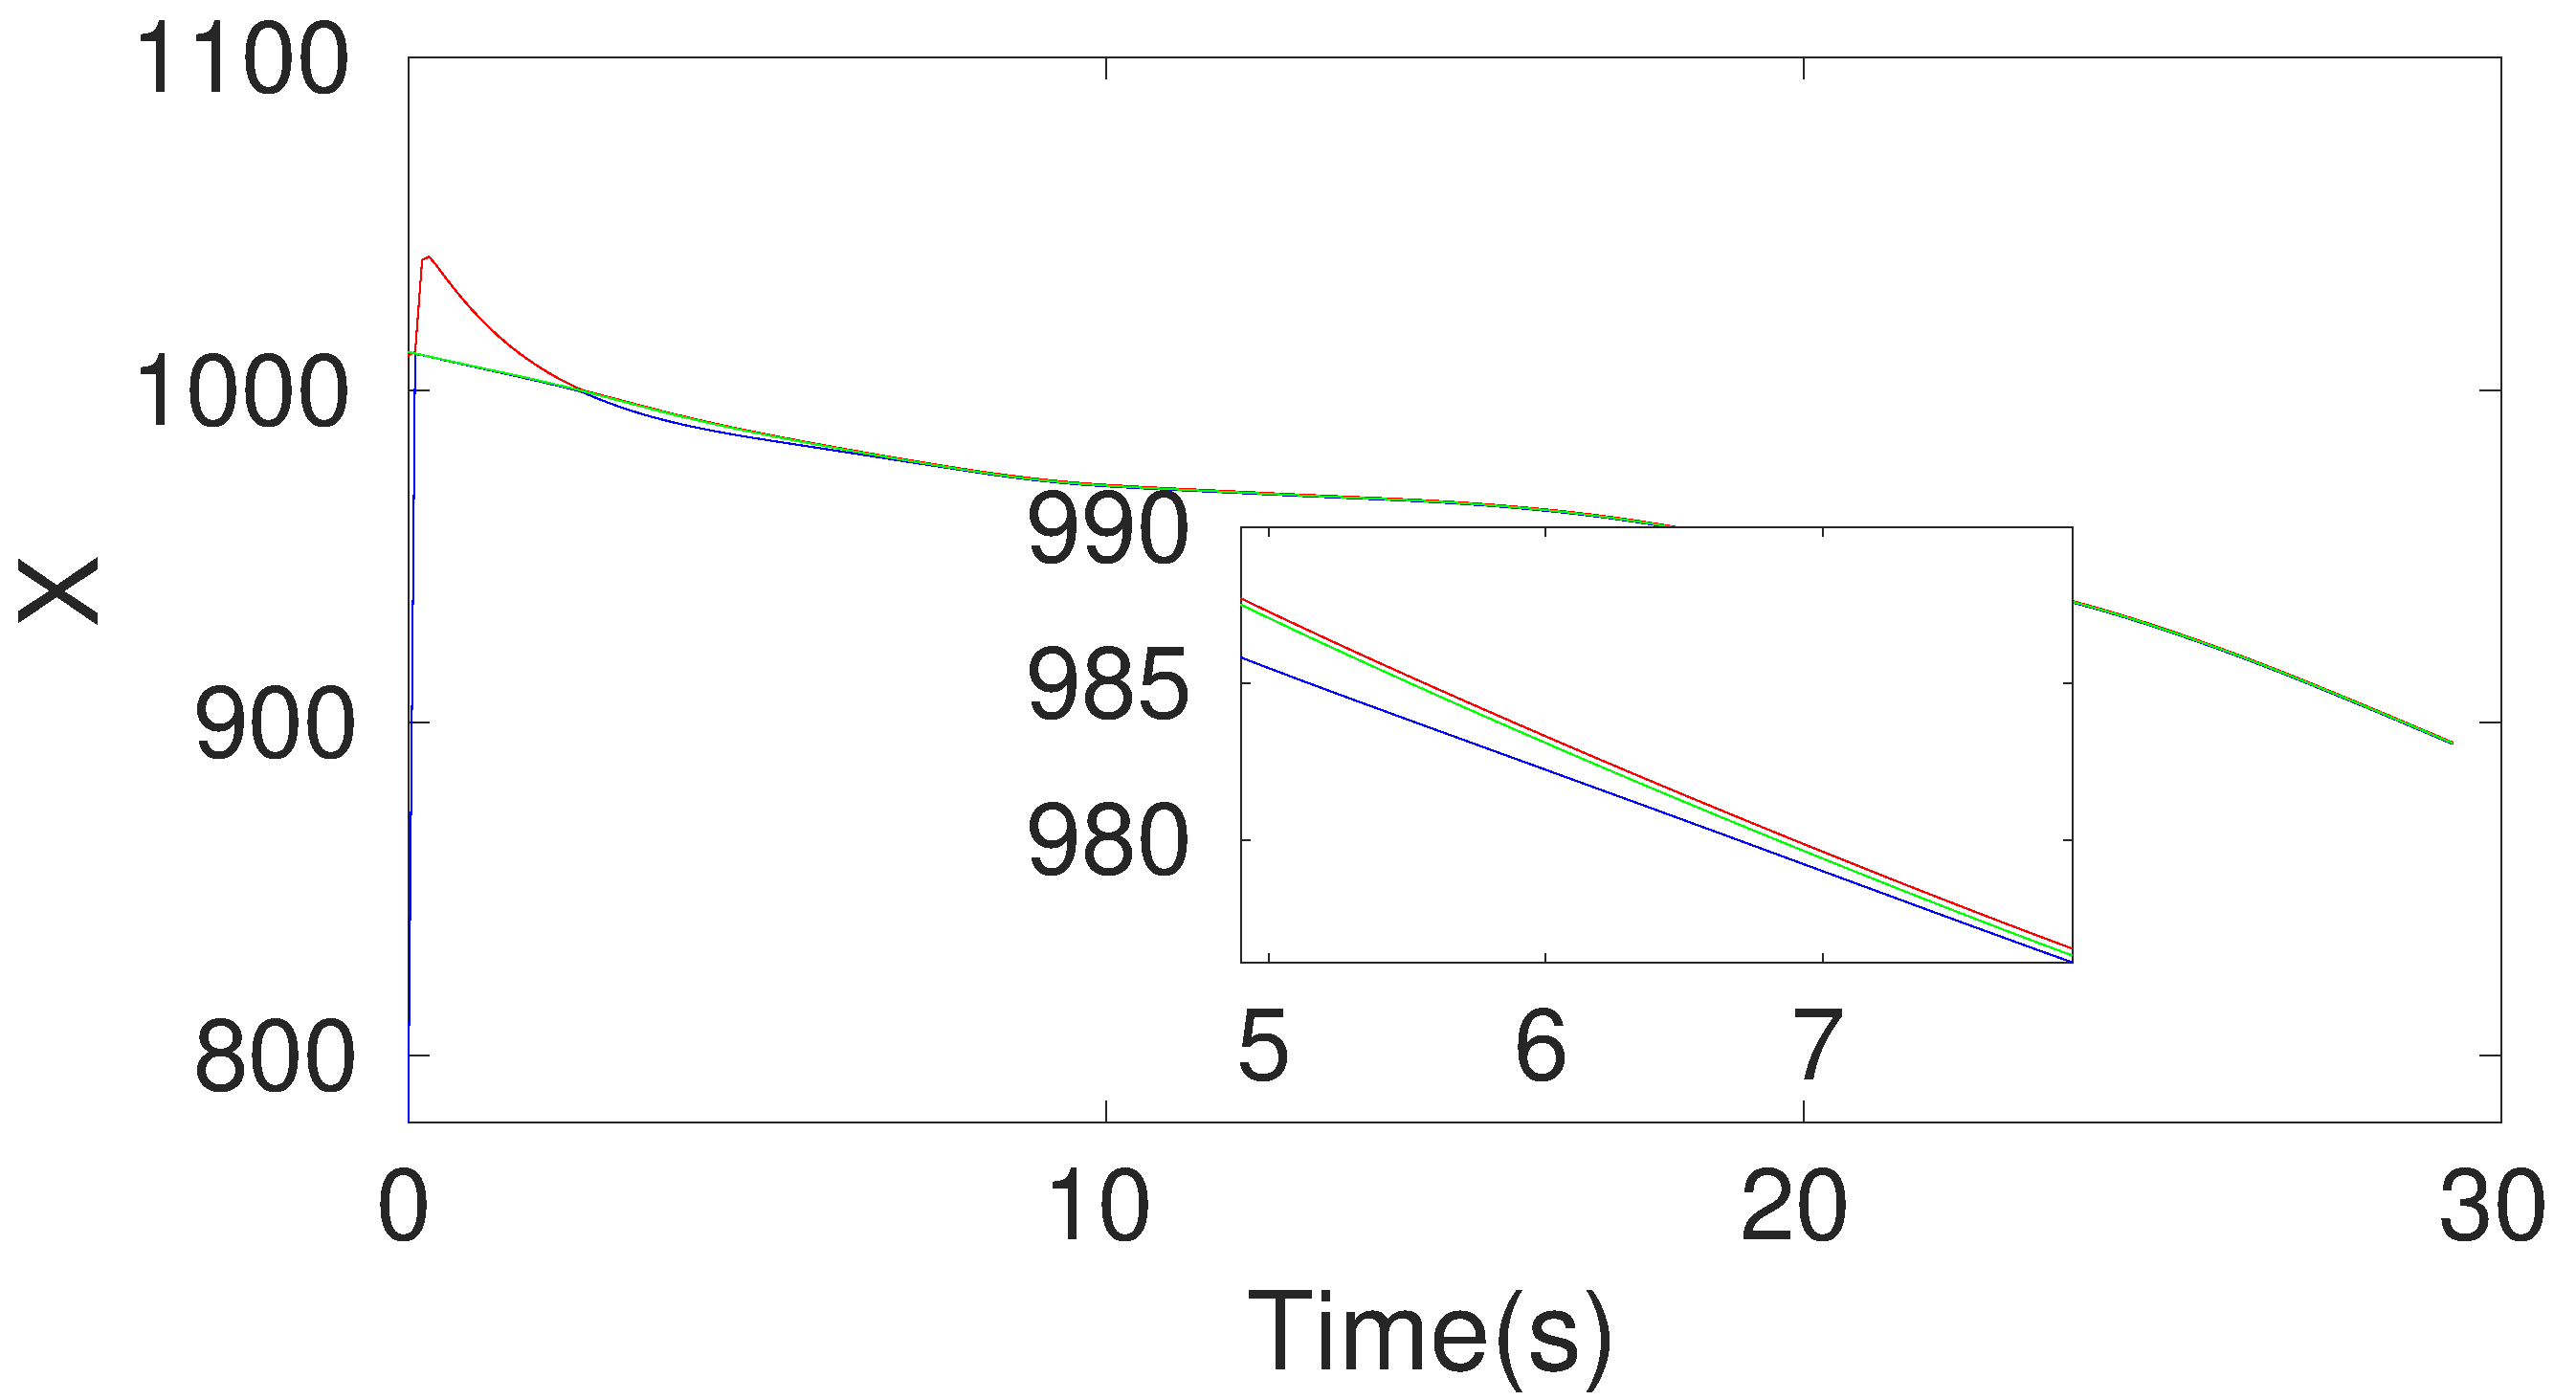
\includegraphics[width=\linewidth]{figures/Prad/s3pmpradX}
\end{subfigure}
\begin{subfigure}{.5\linewidth}
\centering
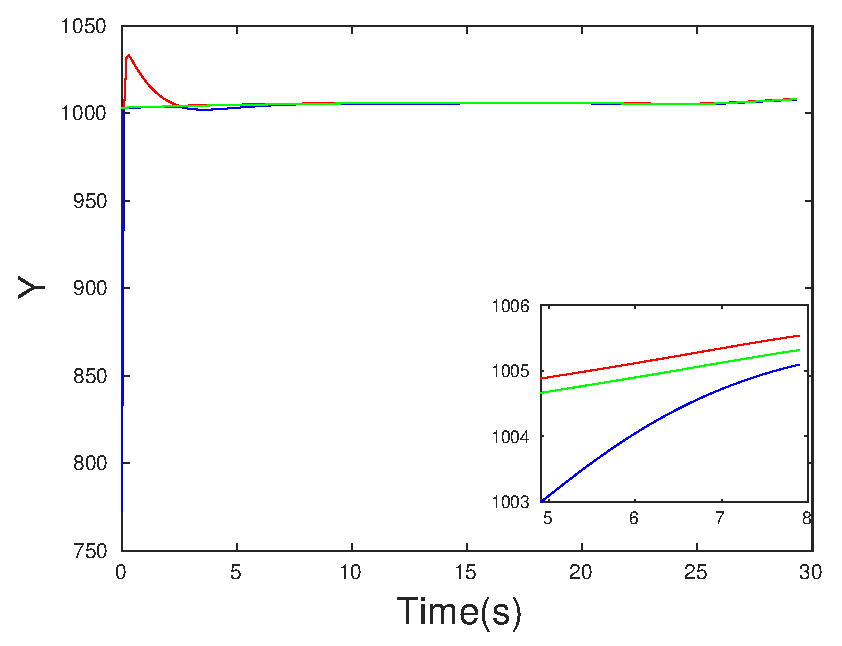
\includegraphics[width=\linewidth]{figures/Prad/s3pmpradY}
\end{subfigure}
\begin{subfigure}{.5\linewidth}
\centering
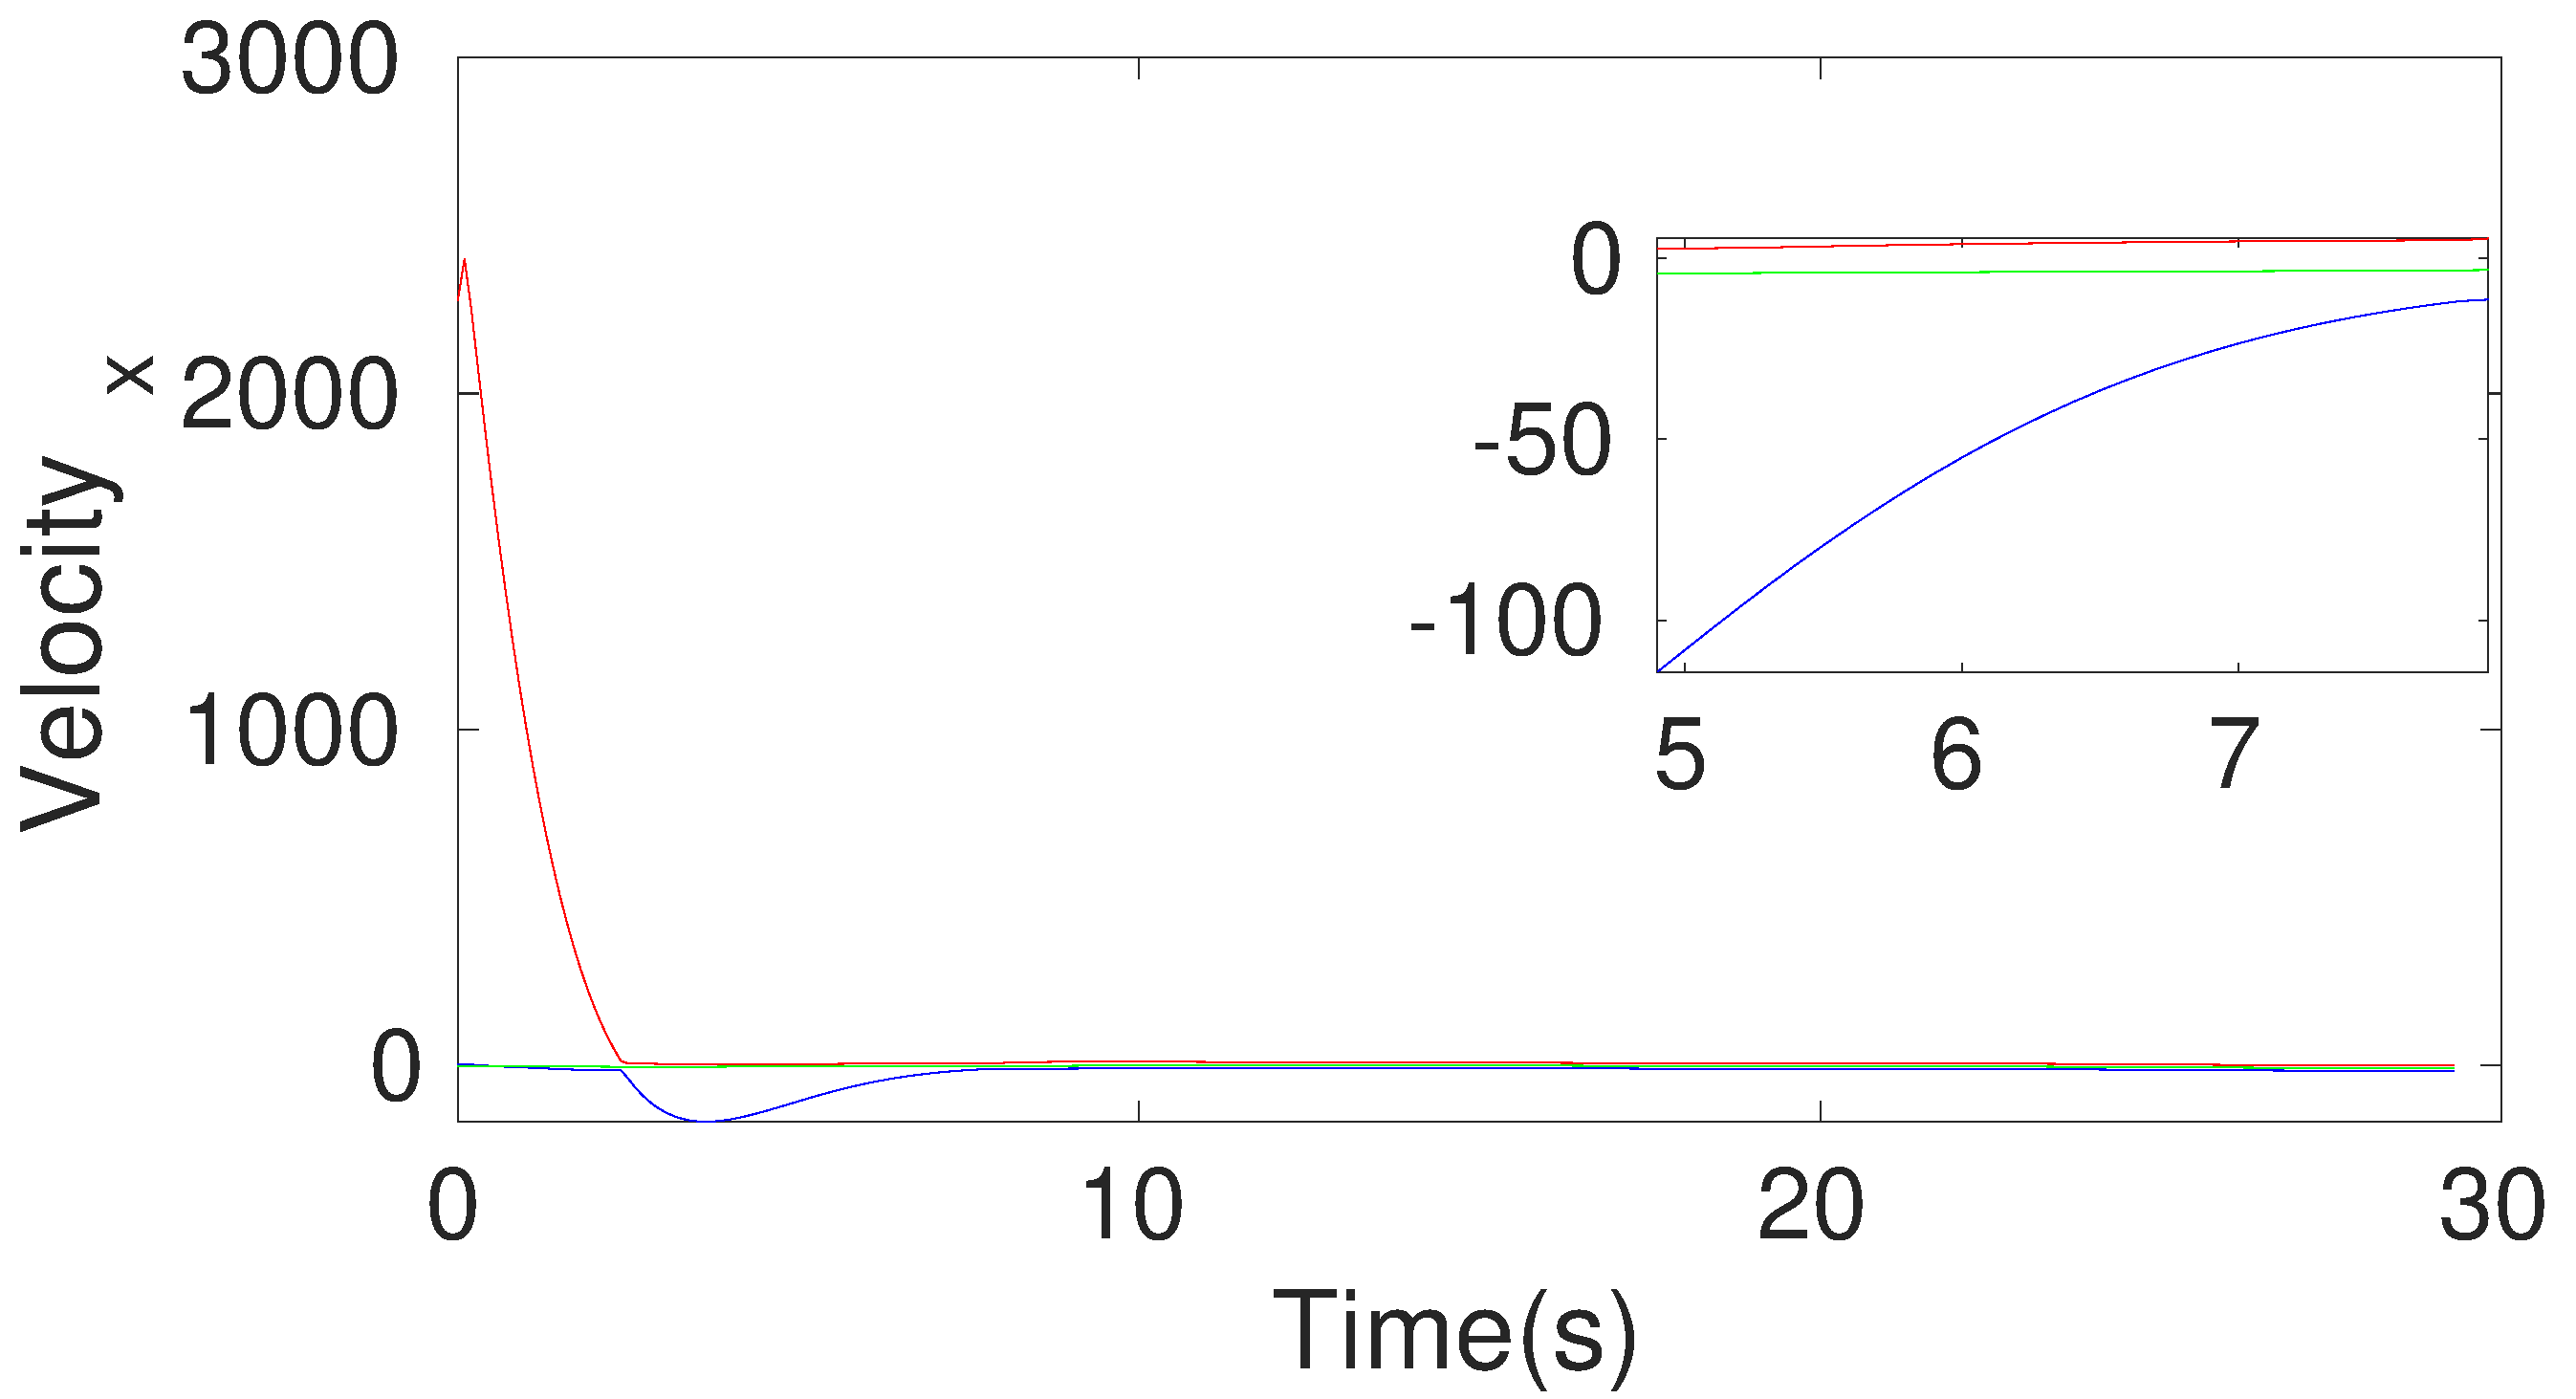
\includegraphics[width=\linewidth]{figures/Prad/s3pmpradVelocity_x}
\end{subfigure}
\begin{subfigure}{.5\linewidth}
\centering
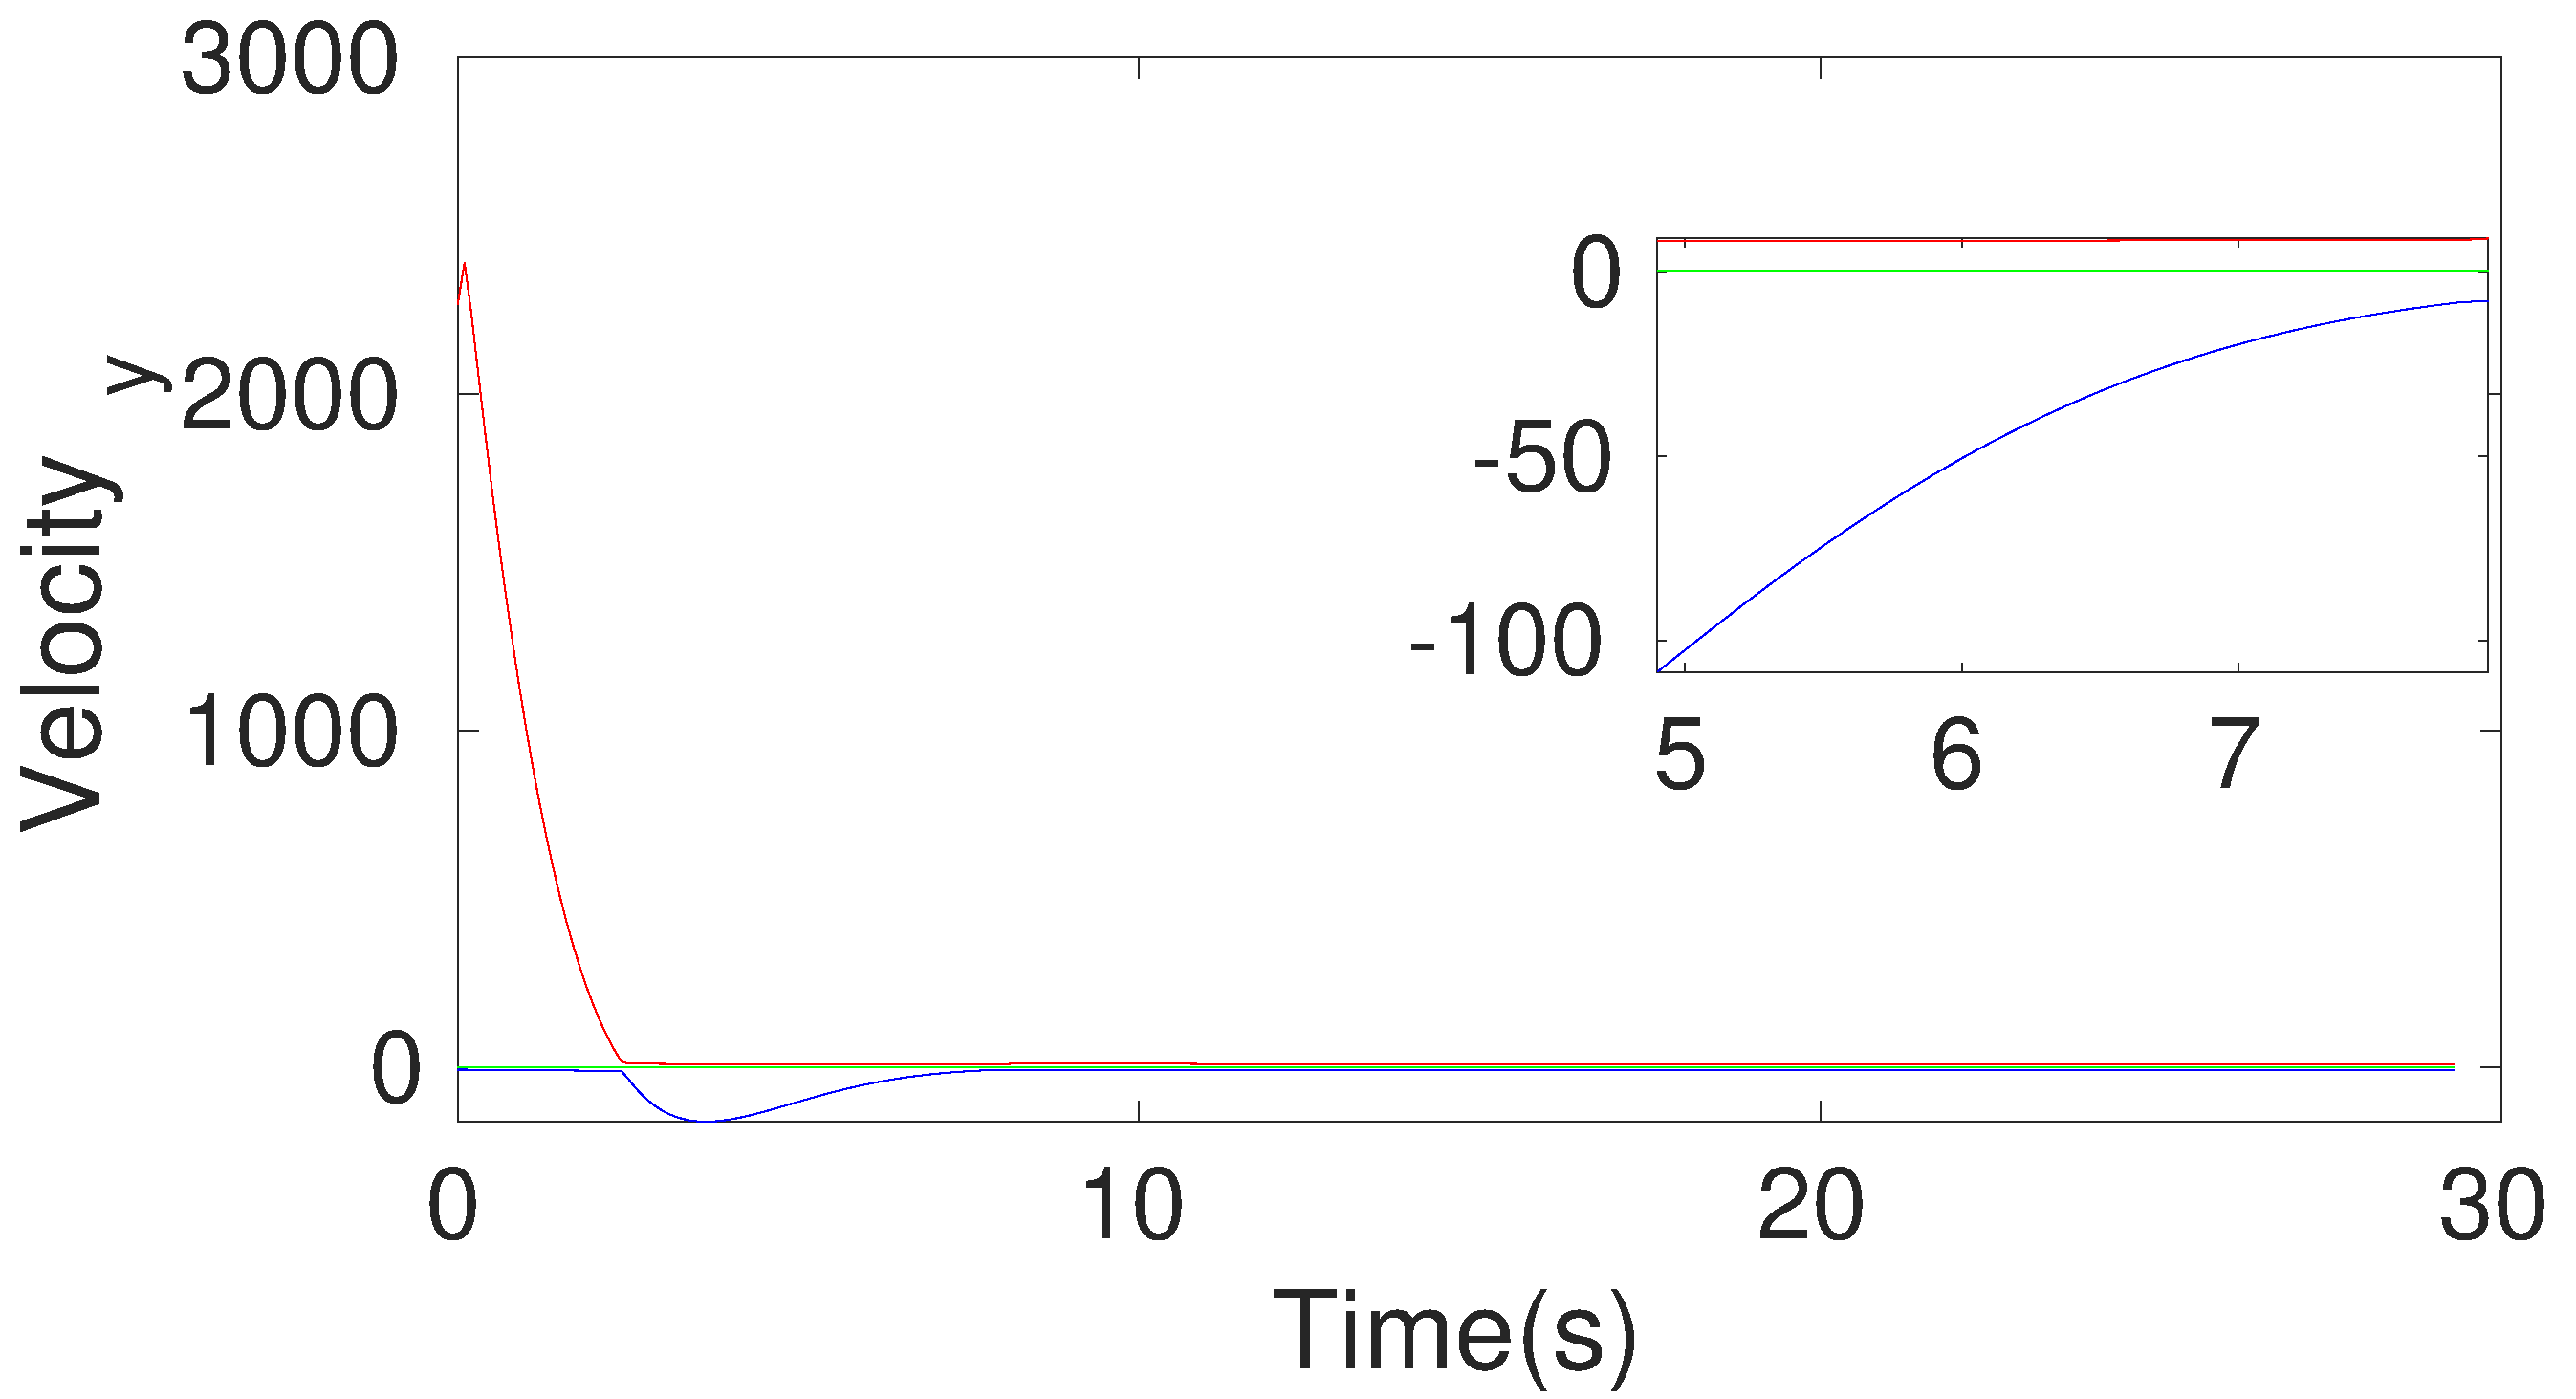
\includegraphics[width=\linewidth]{figures/Prad/s3pmpradVelocity_y}
\end{subfigure}
\begin{subfigure}{.5\linewidth}
\centering
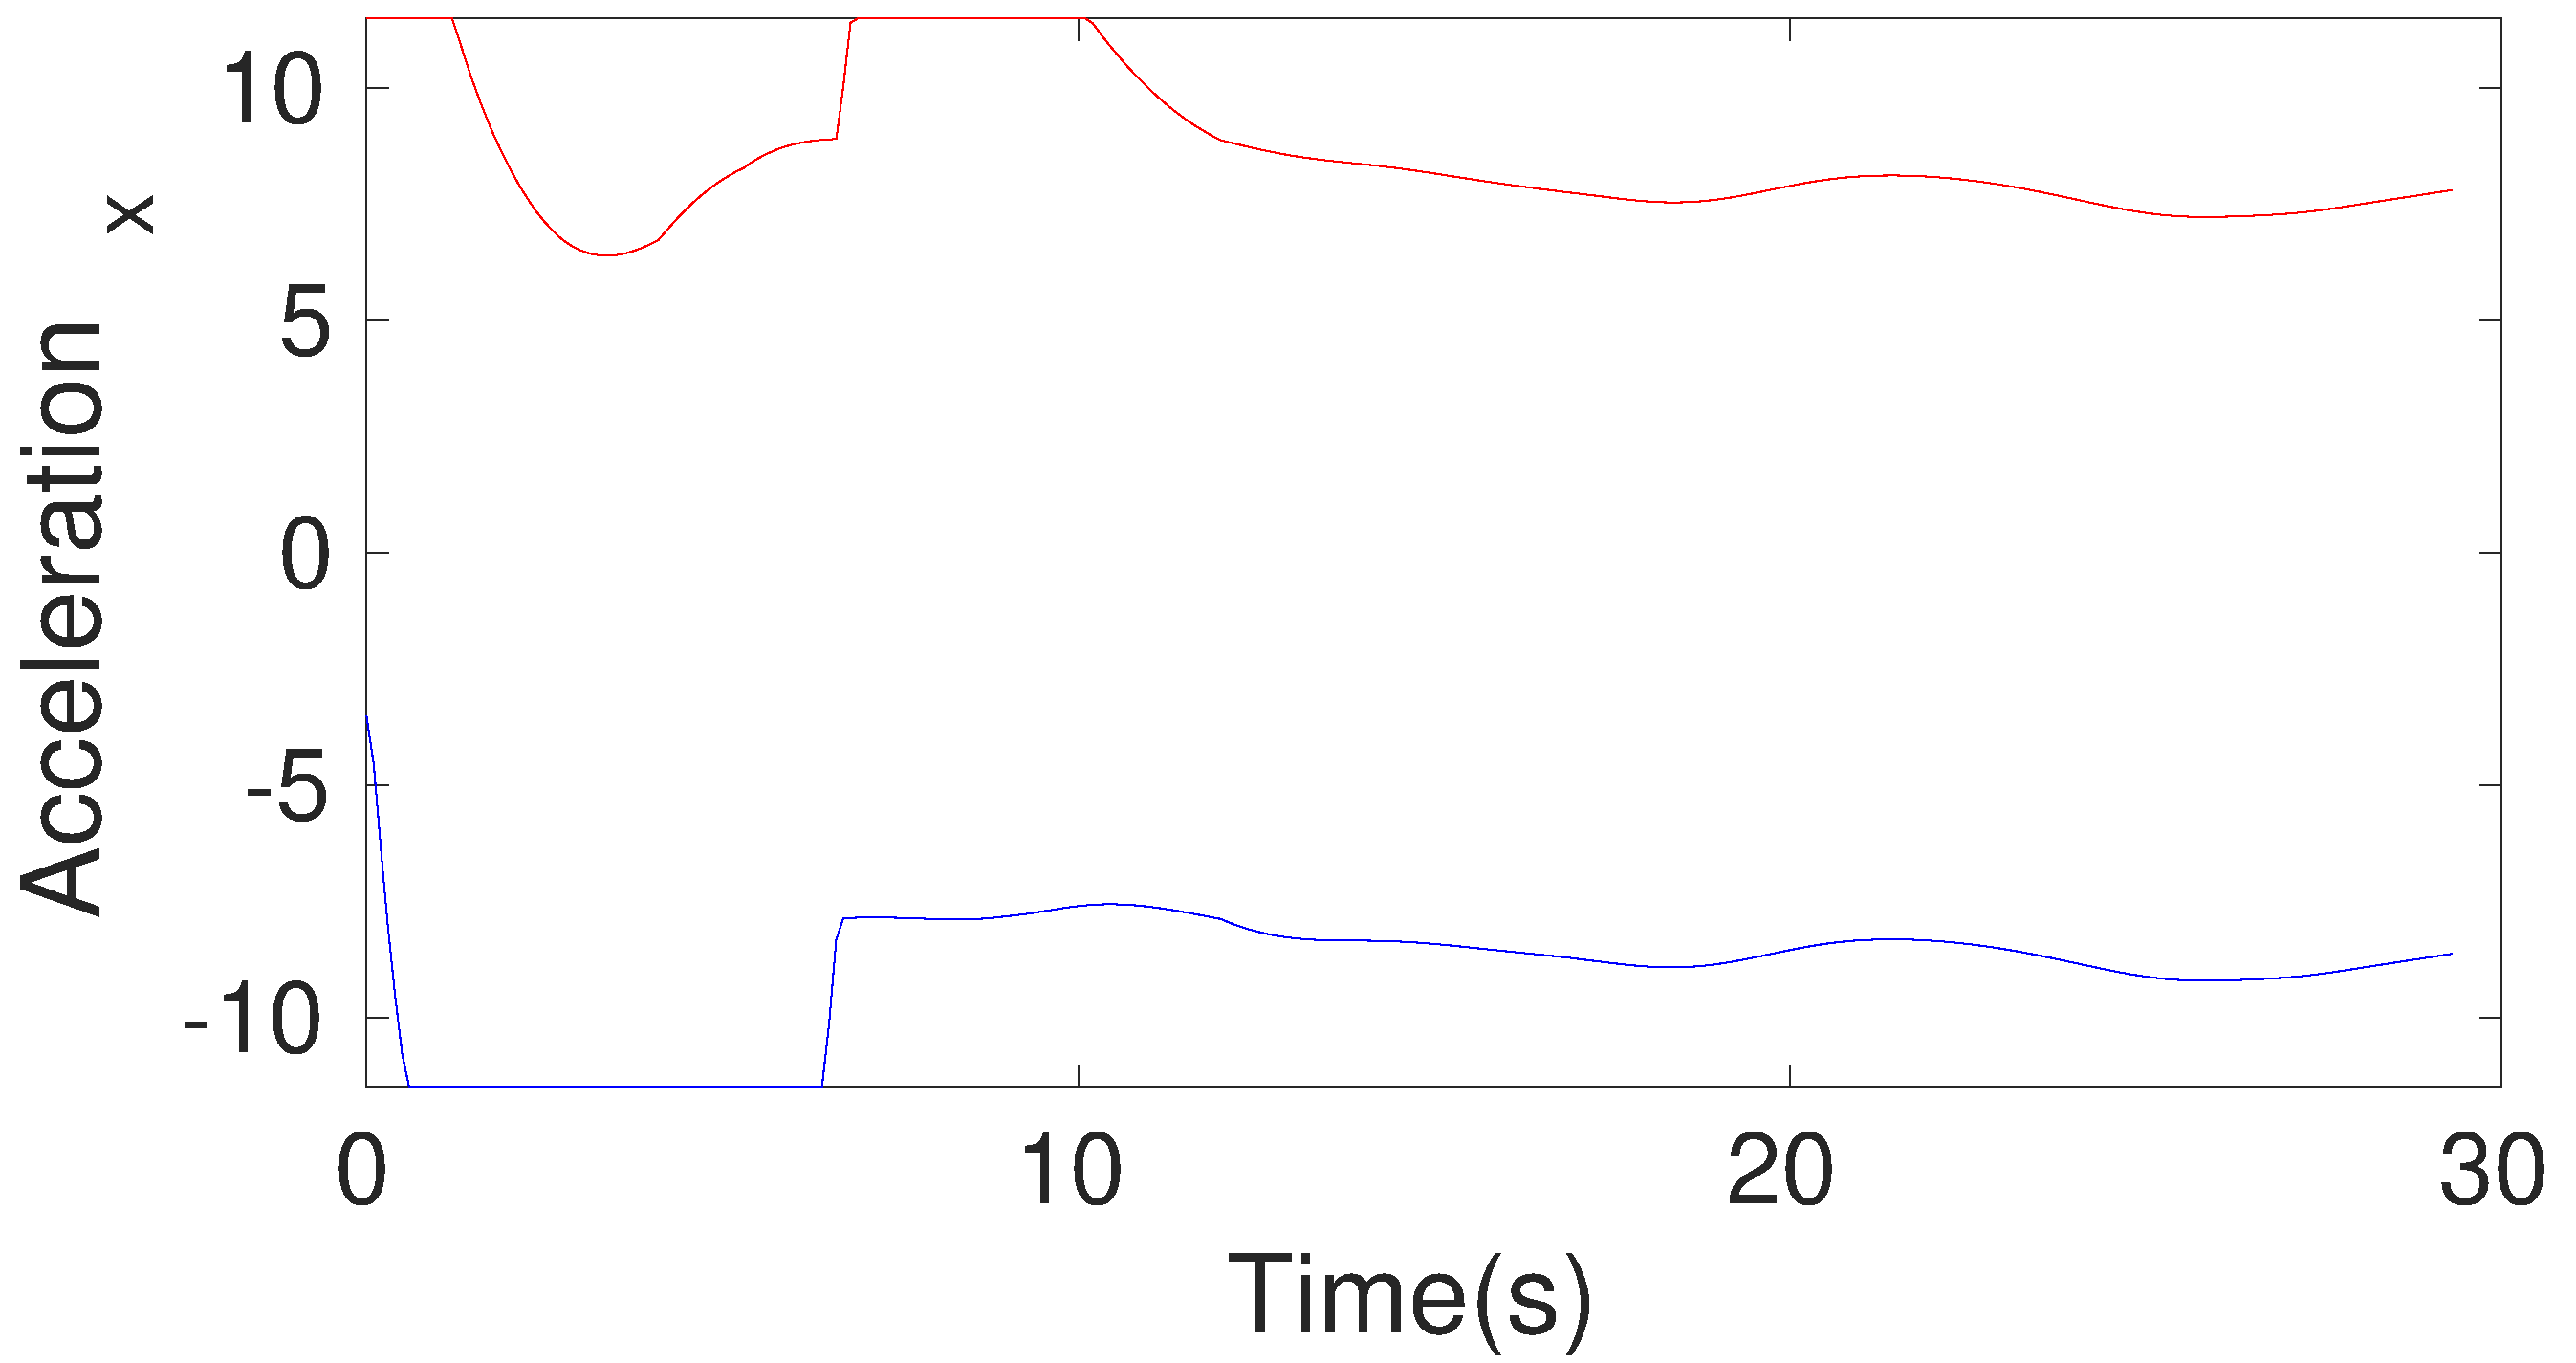
\includegraphics[width=\linewidth]{figures/Prad/s3pmpradAcceleration_x}
\end{subfigure}
\begin{subfigure}{.5\linewidth}
\centering
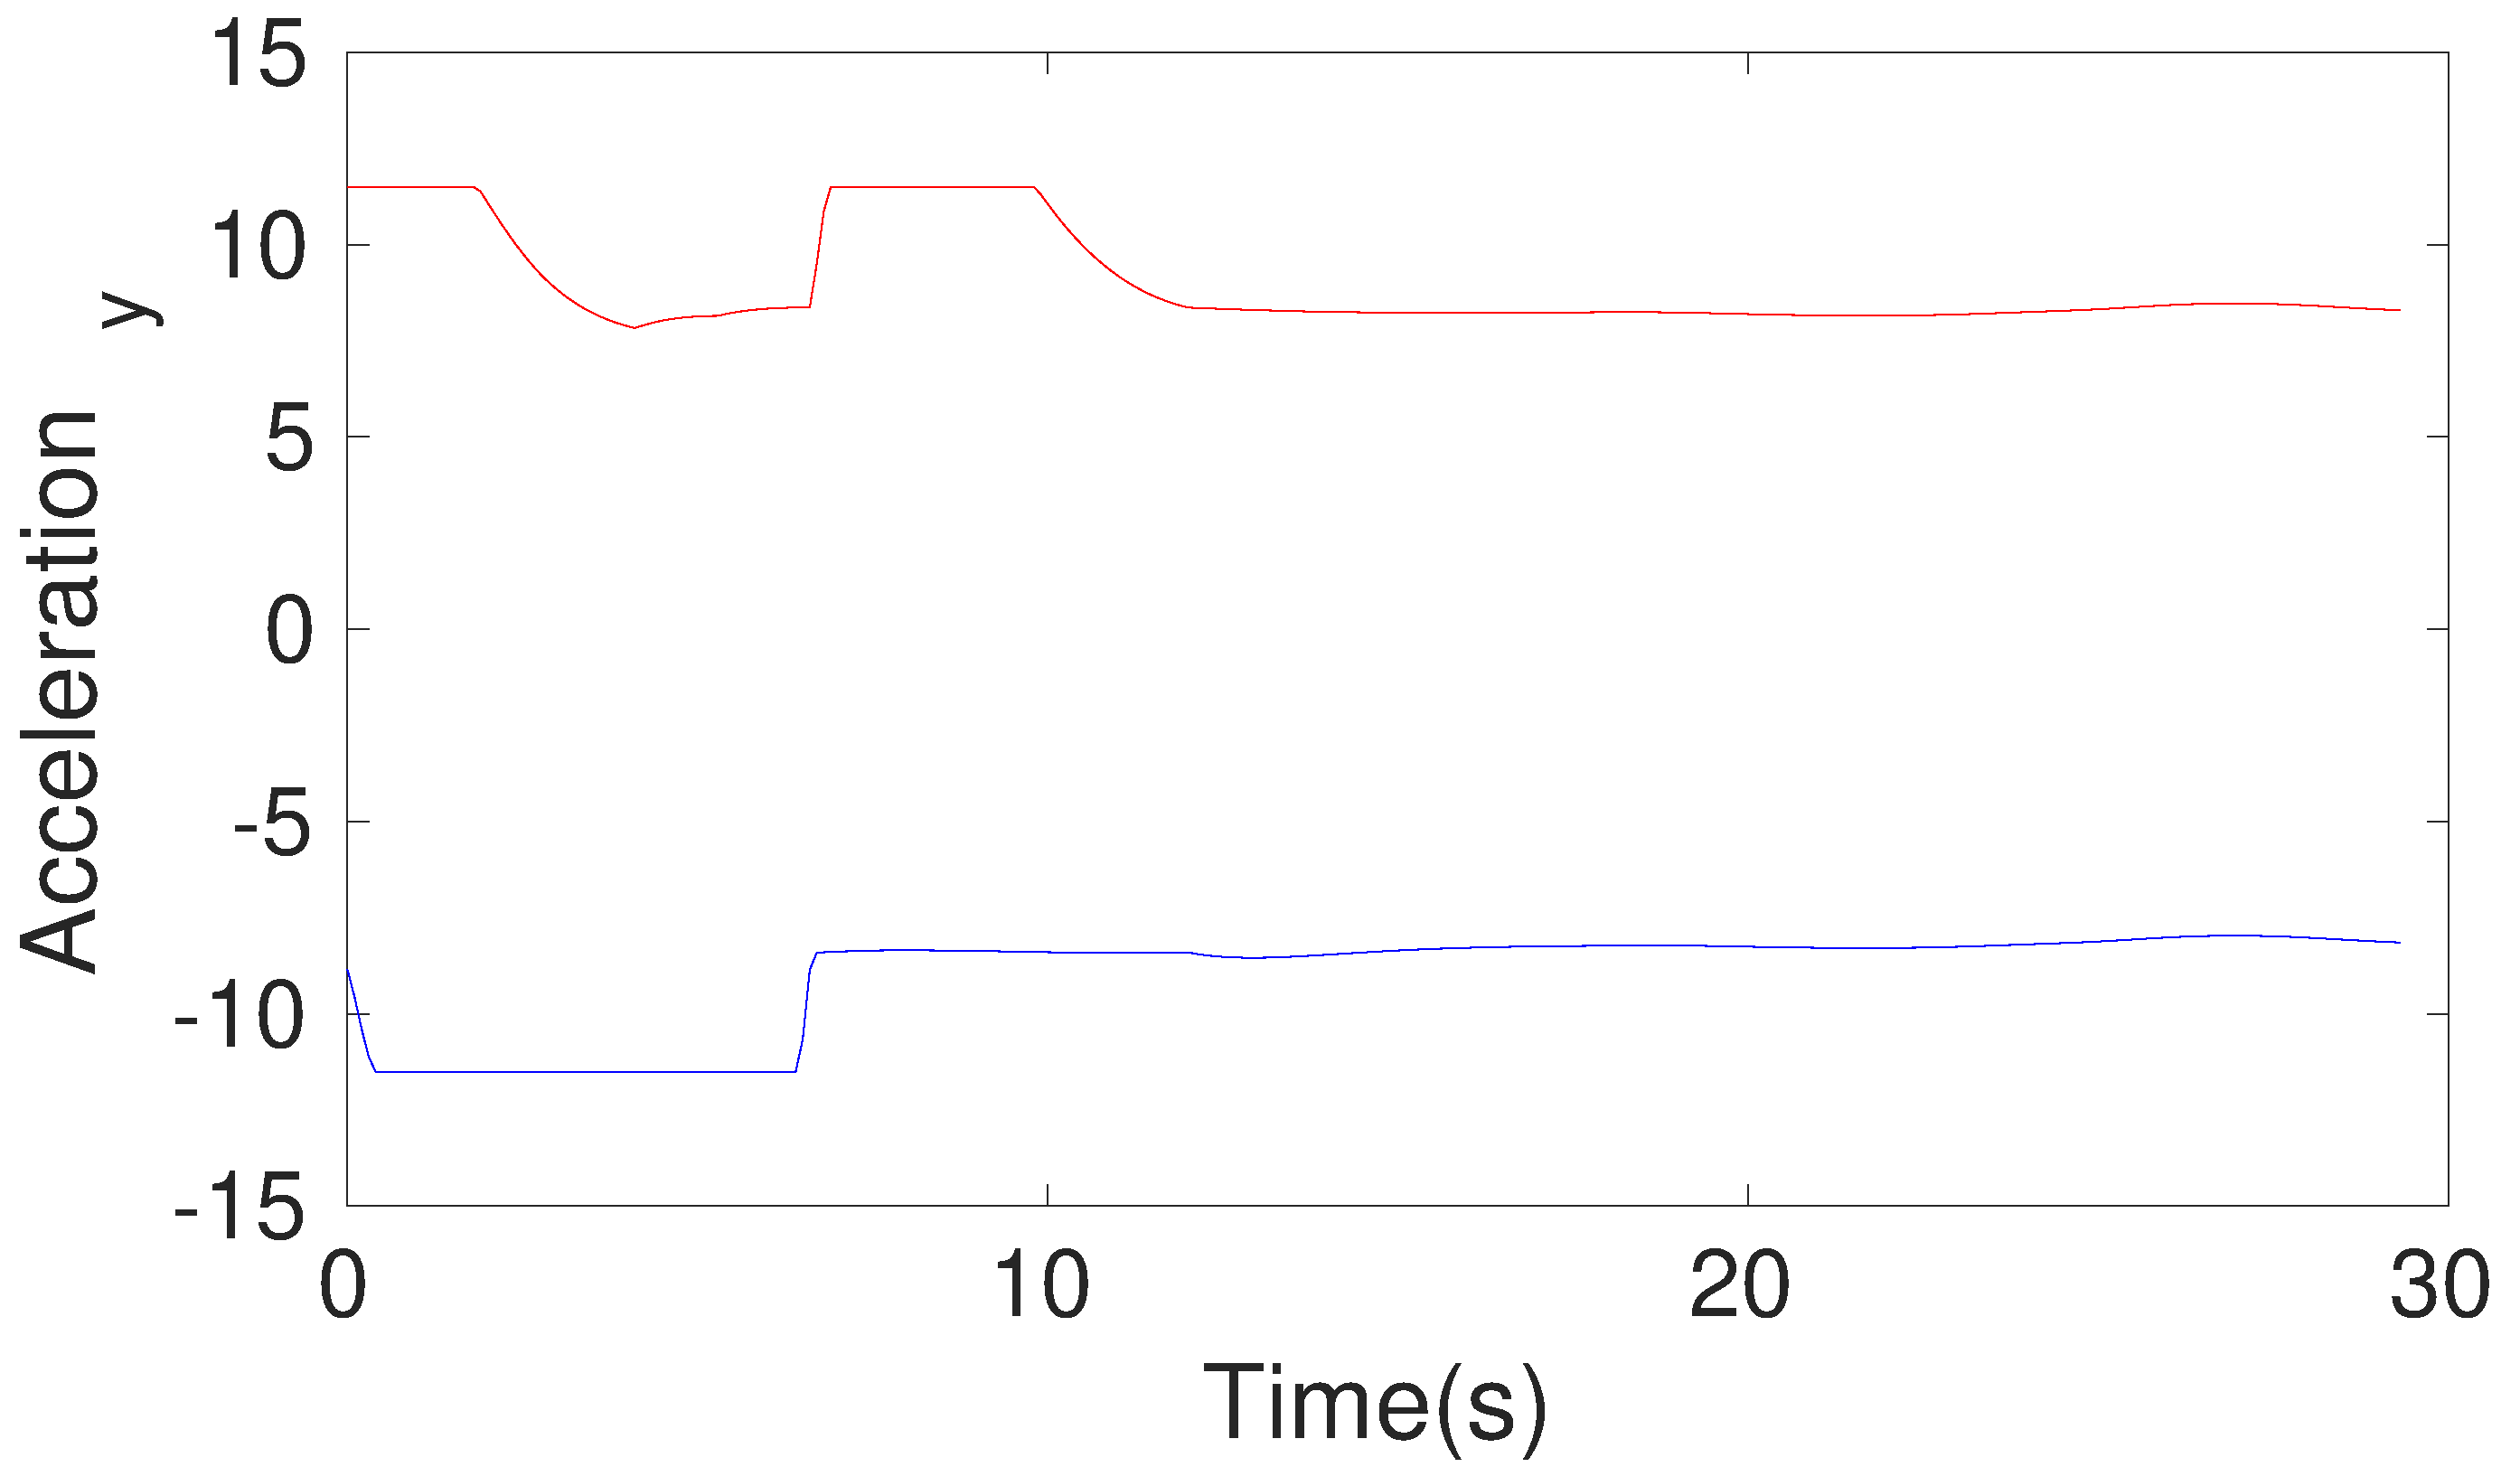
\includegraphics[width=\linewidth]{figures/Prad/s3pmpradAcceleration_y}
\end{subfigure}
\caption{Estimation using the P-radius and the point-mass model}
\end{figure}


\clearpage
\subsection{Interval Observer using H-$\infty$}\label{eresult:hinf}
\FloatBarrier
\begin{figure}[!h]
\hspace*{\fill} 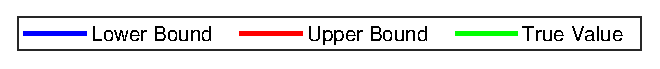
\includegraphics[scale=0.8]{figures/legend}\\\\
\begin{subfigure}{.5\linewidth}
\centering
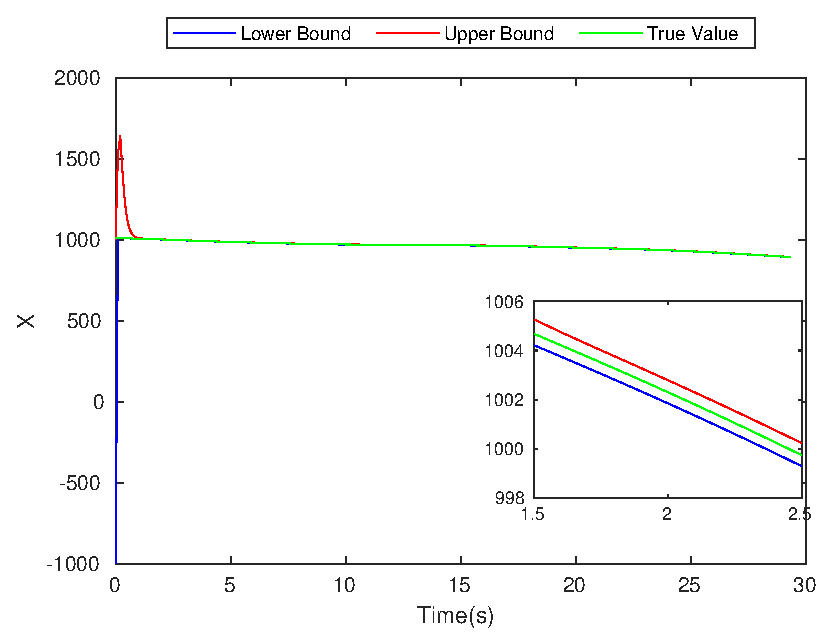
\includegraphics[width=\linewidth]{figures/HInf/s3cvHInfX}
\end{subfigure}
\begin{subfigure}{.5\linewidth}
\centering
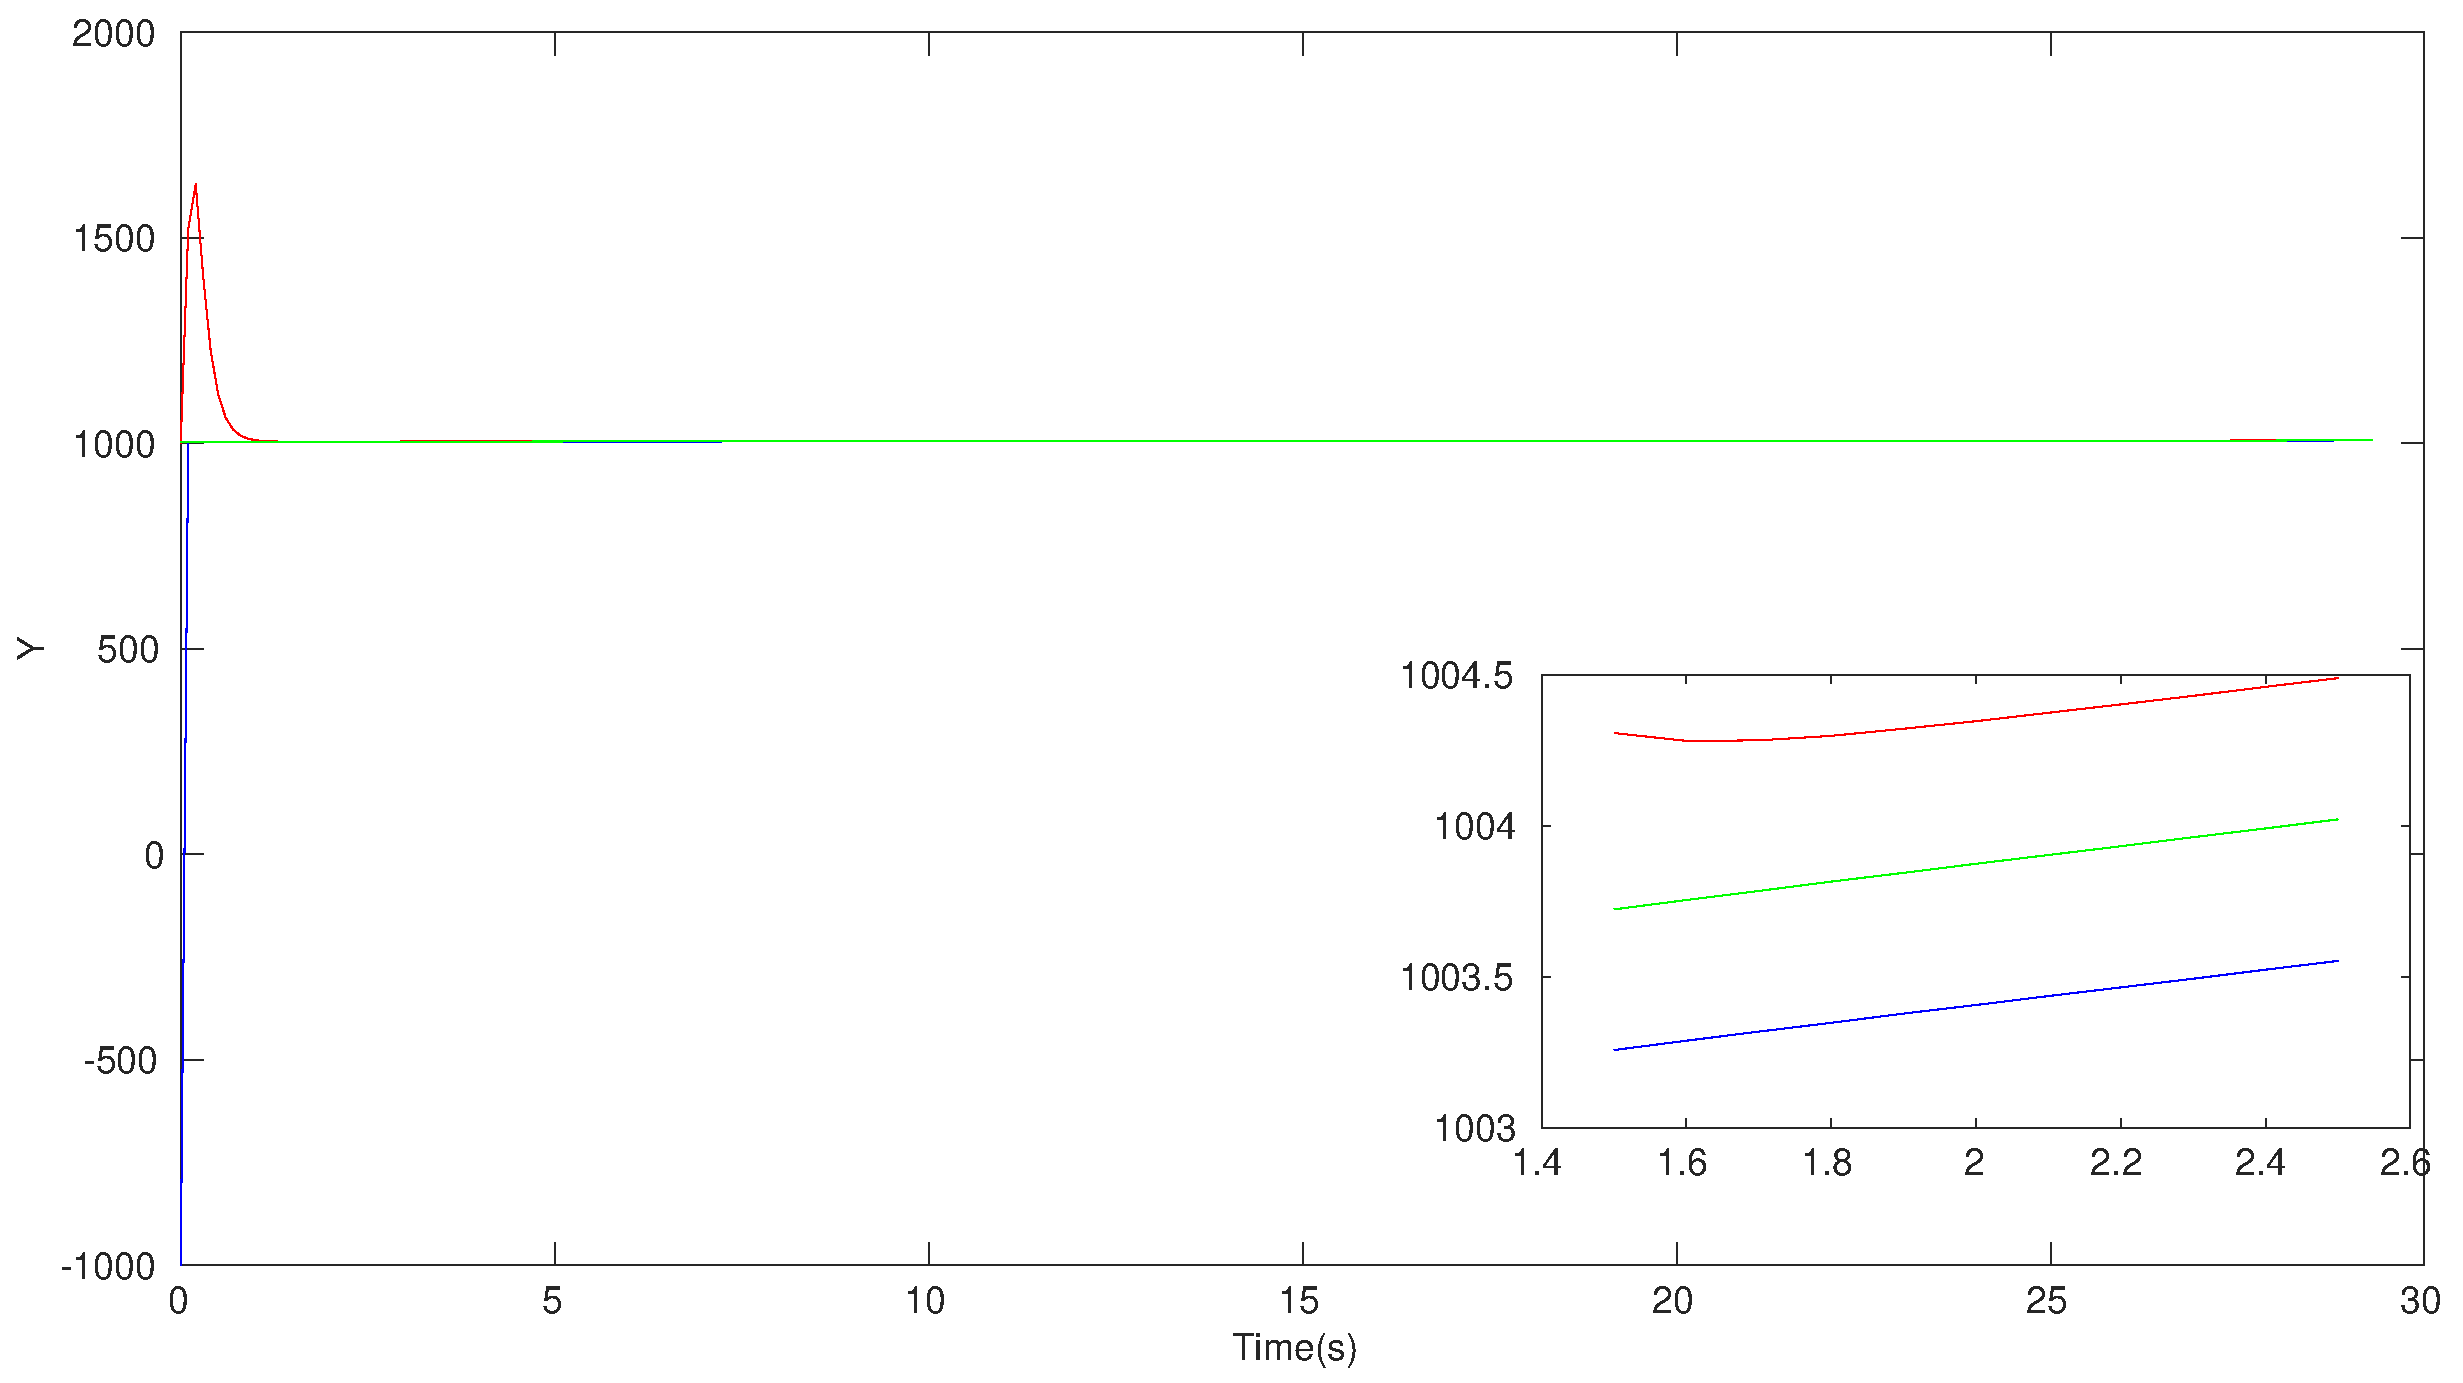
\includegraphics[width=\linewidth]{figures/HInf/s3cvHInfY}
\end{subfigure}
\begin{subfigure}{.5\linewidth}
\centering
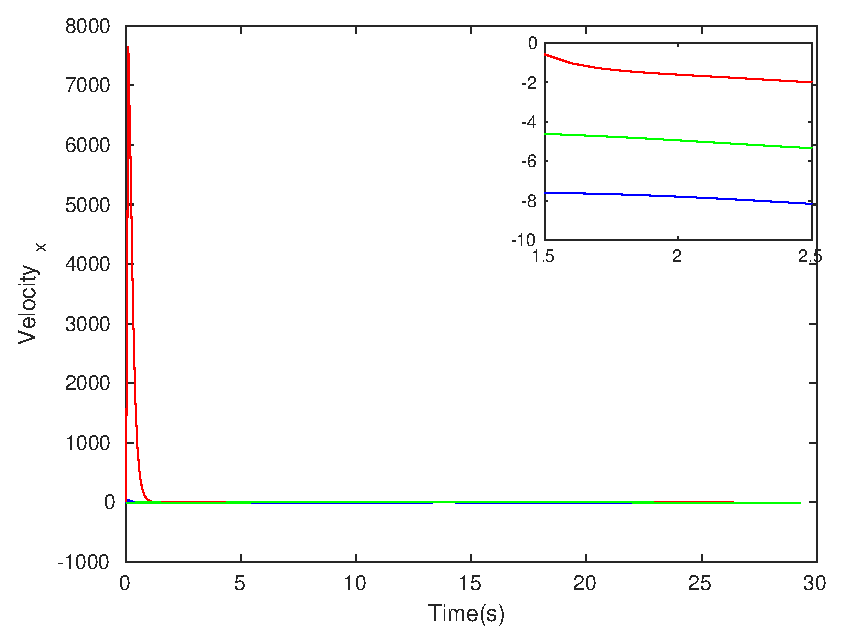
\includegraphics[width=\linewidth]{figures/HInf/s3cvHInfVelocity_x}
\end{subfigure}
\begin{subfigure}{.5\linewidth}
\centering
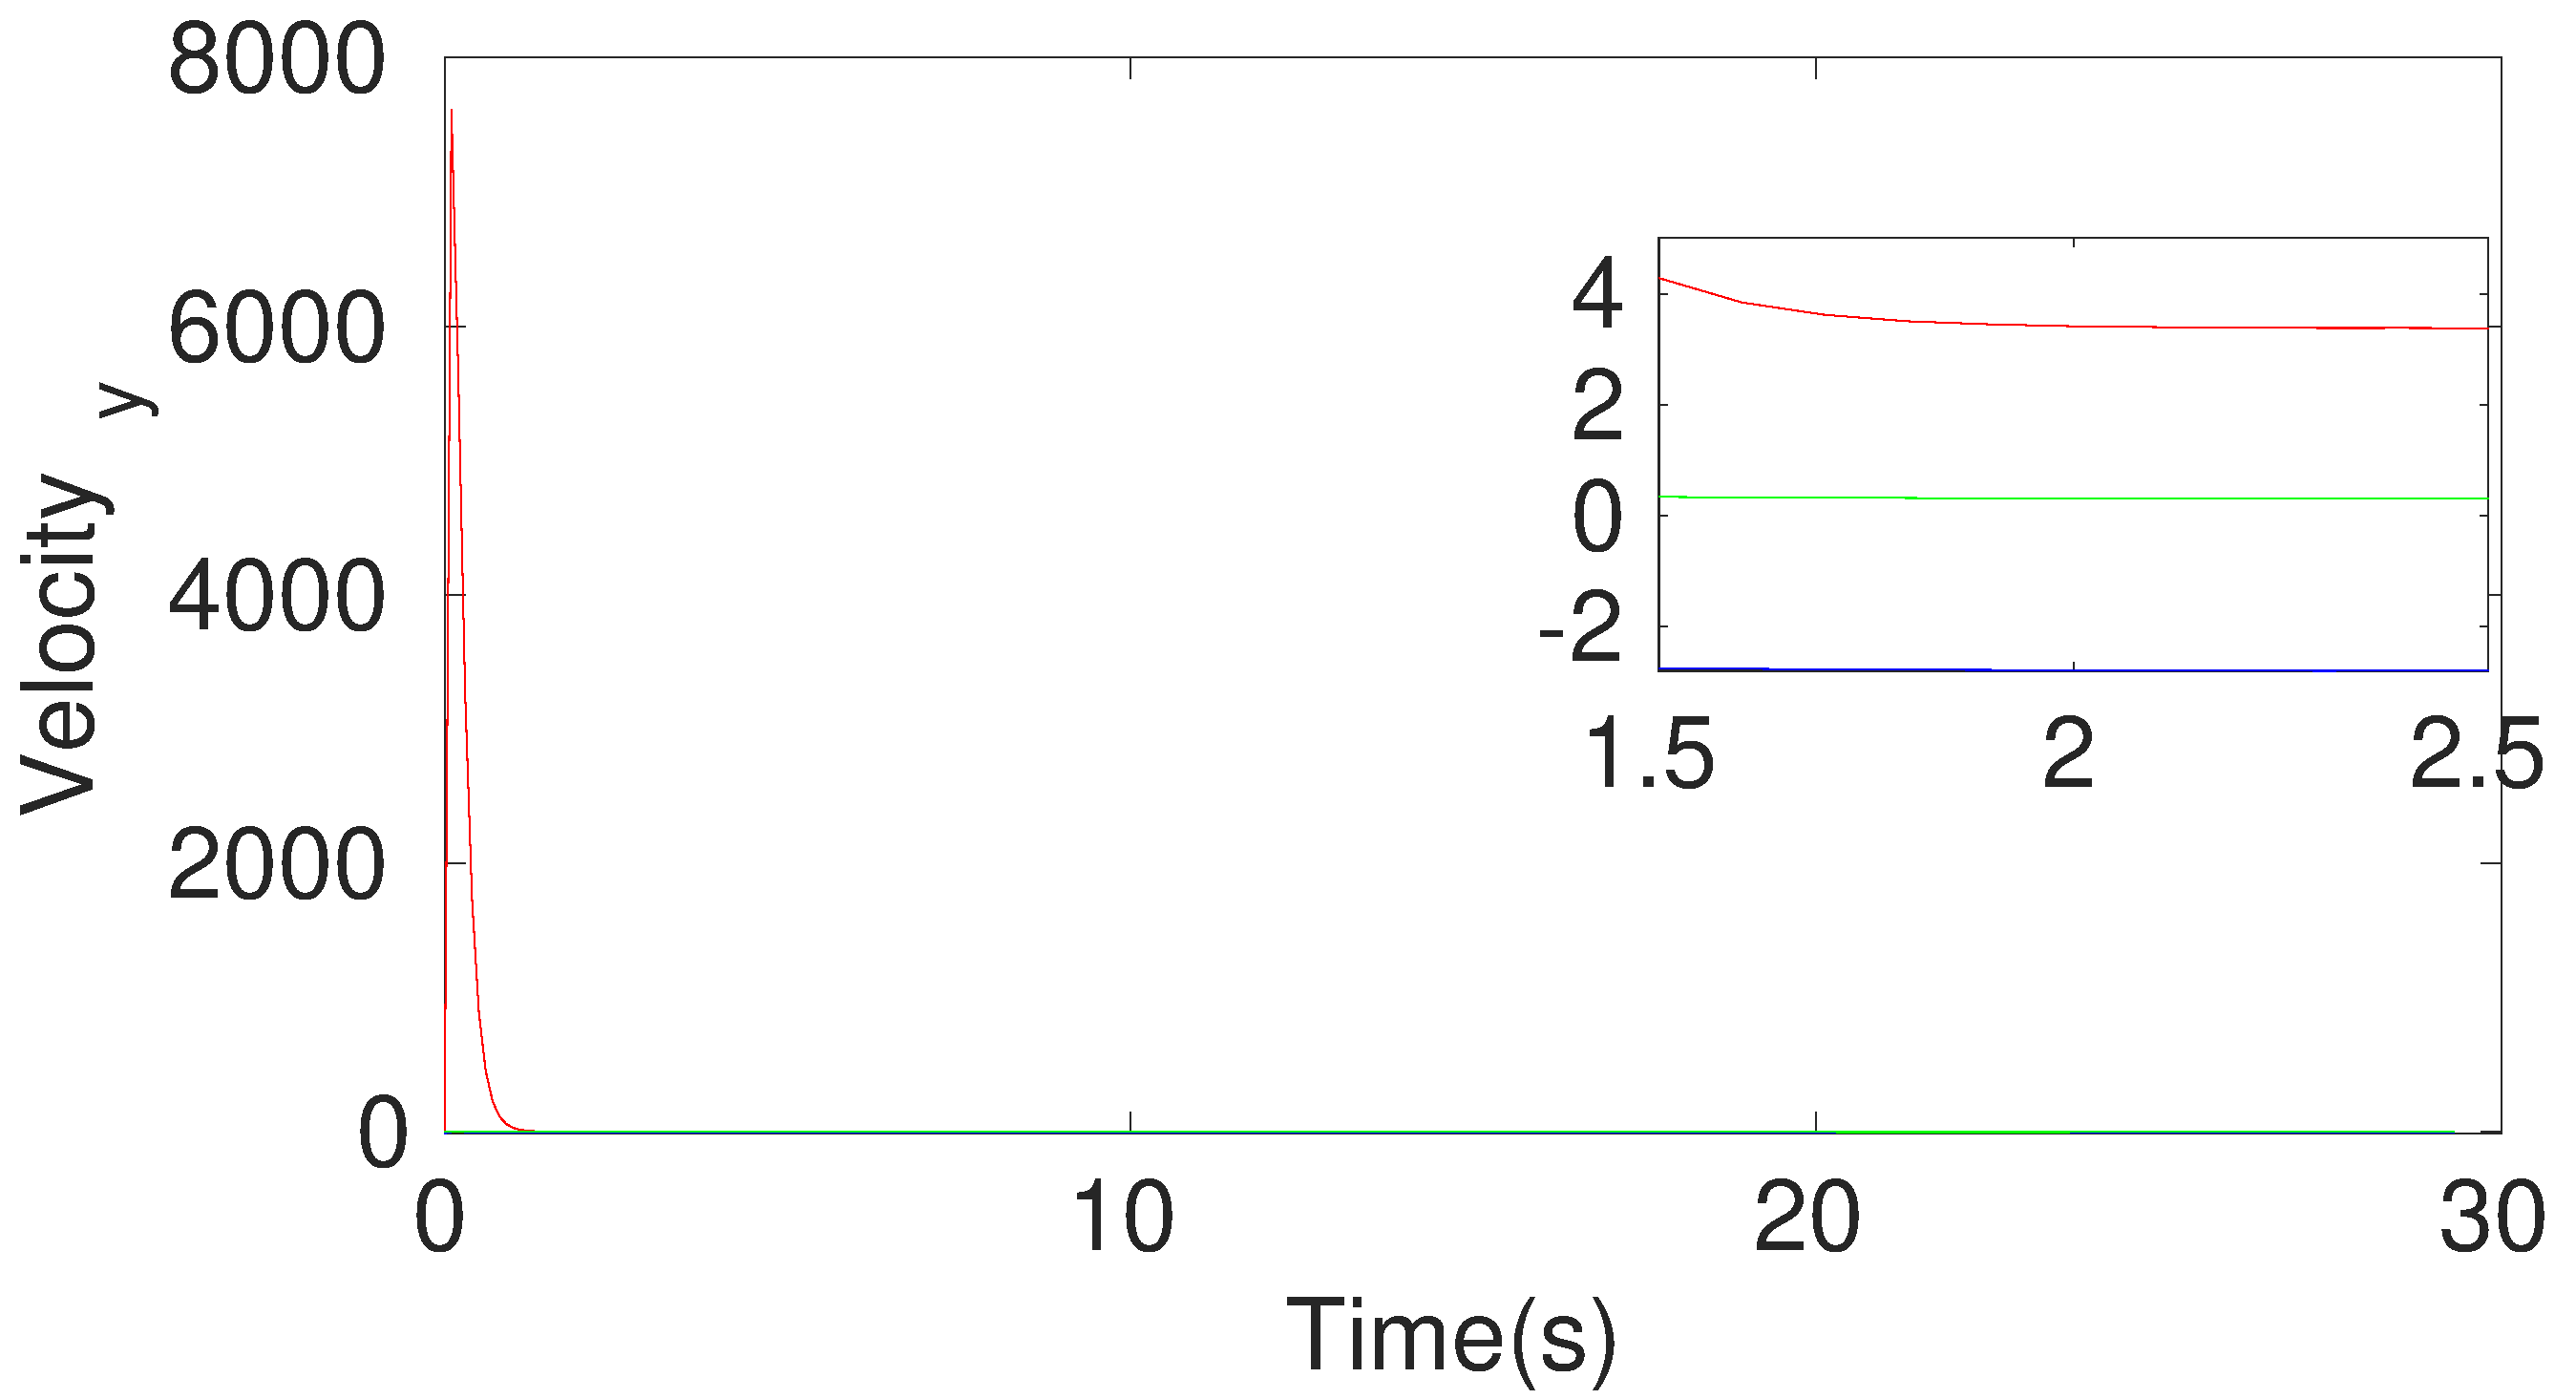
\includegraphics[width=\linewidth]{figures/HInf/s3cvHInfVelocity_y}
\end{subfigure}
\caption{Estimation using H-$\infty$ observer and the constant velocity model}
\end{figure}

\begin{figure}[!h]
\hspace*{\fill} 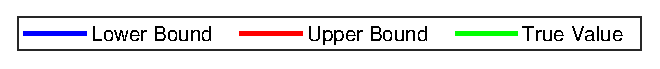
\includegraphics[scale=0.8]{figures/legend}\\\\
\begin{subfigure}{.5\linewidth}
\centering
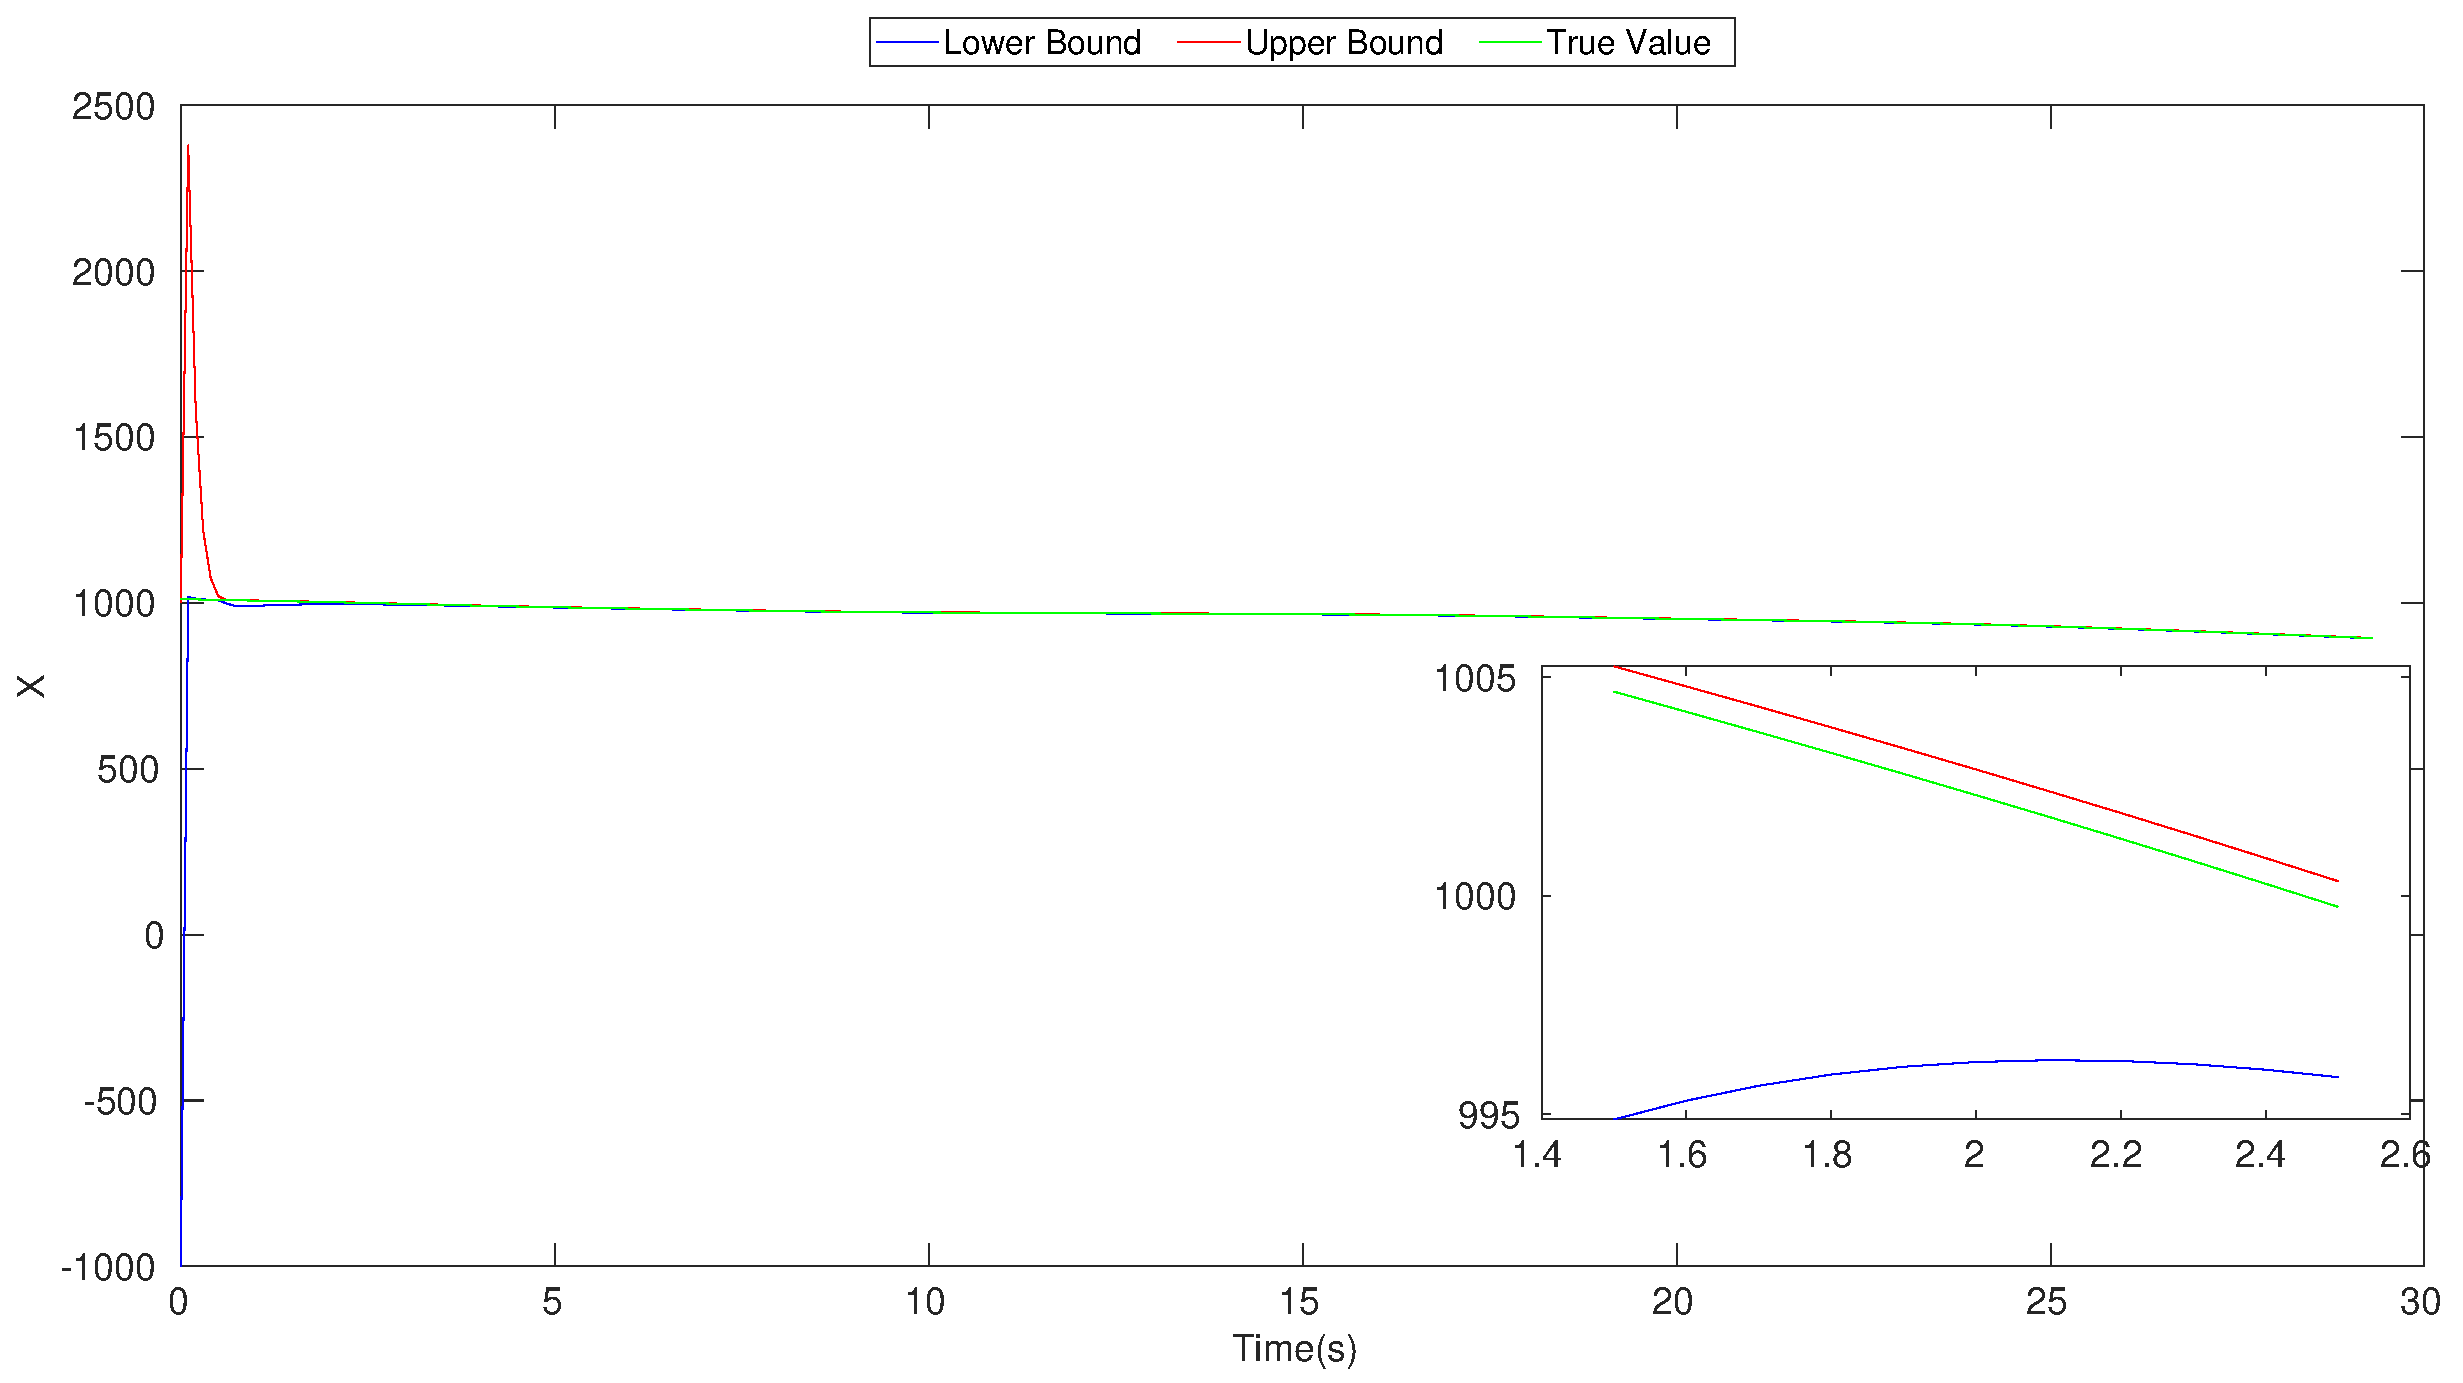
\includegraphics[width=\linewidth]{figures/HInf/s3caHInfX}
\end{subfigure}
\begin{subfigure}{.5\linewidth}
\centering
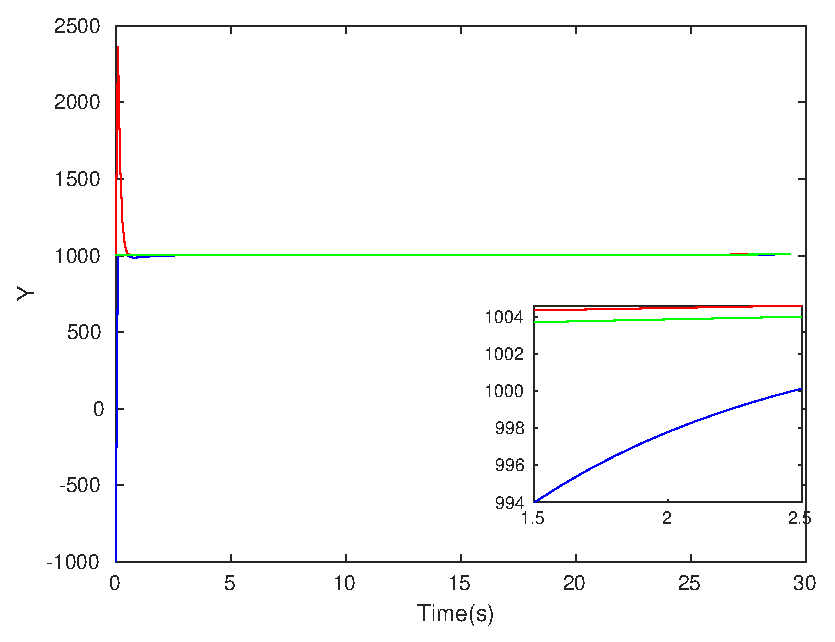
\includegraphics[width=\linewidth]{figures/HInf/s3caHInfY}
\end{subfigure}
\begin{subfigure}{.5\linewidth}
\centering
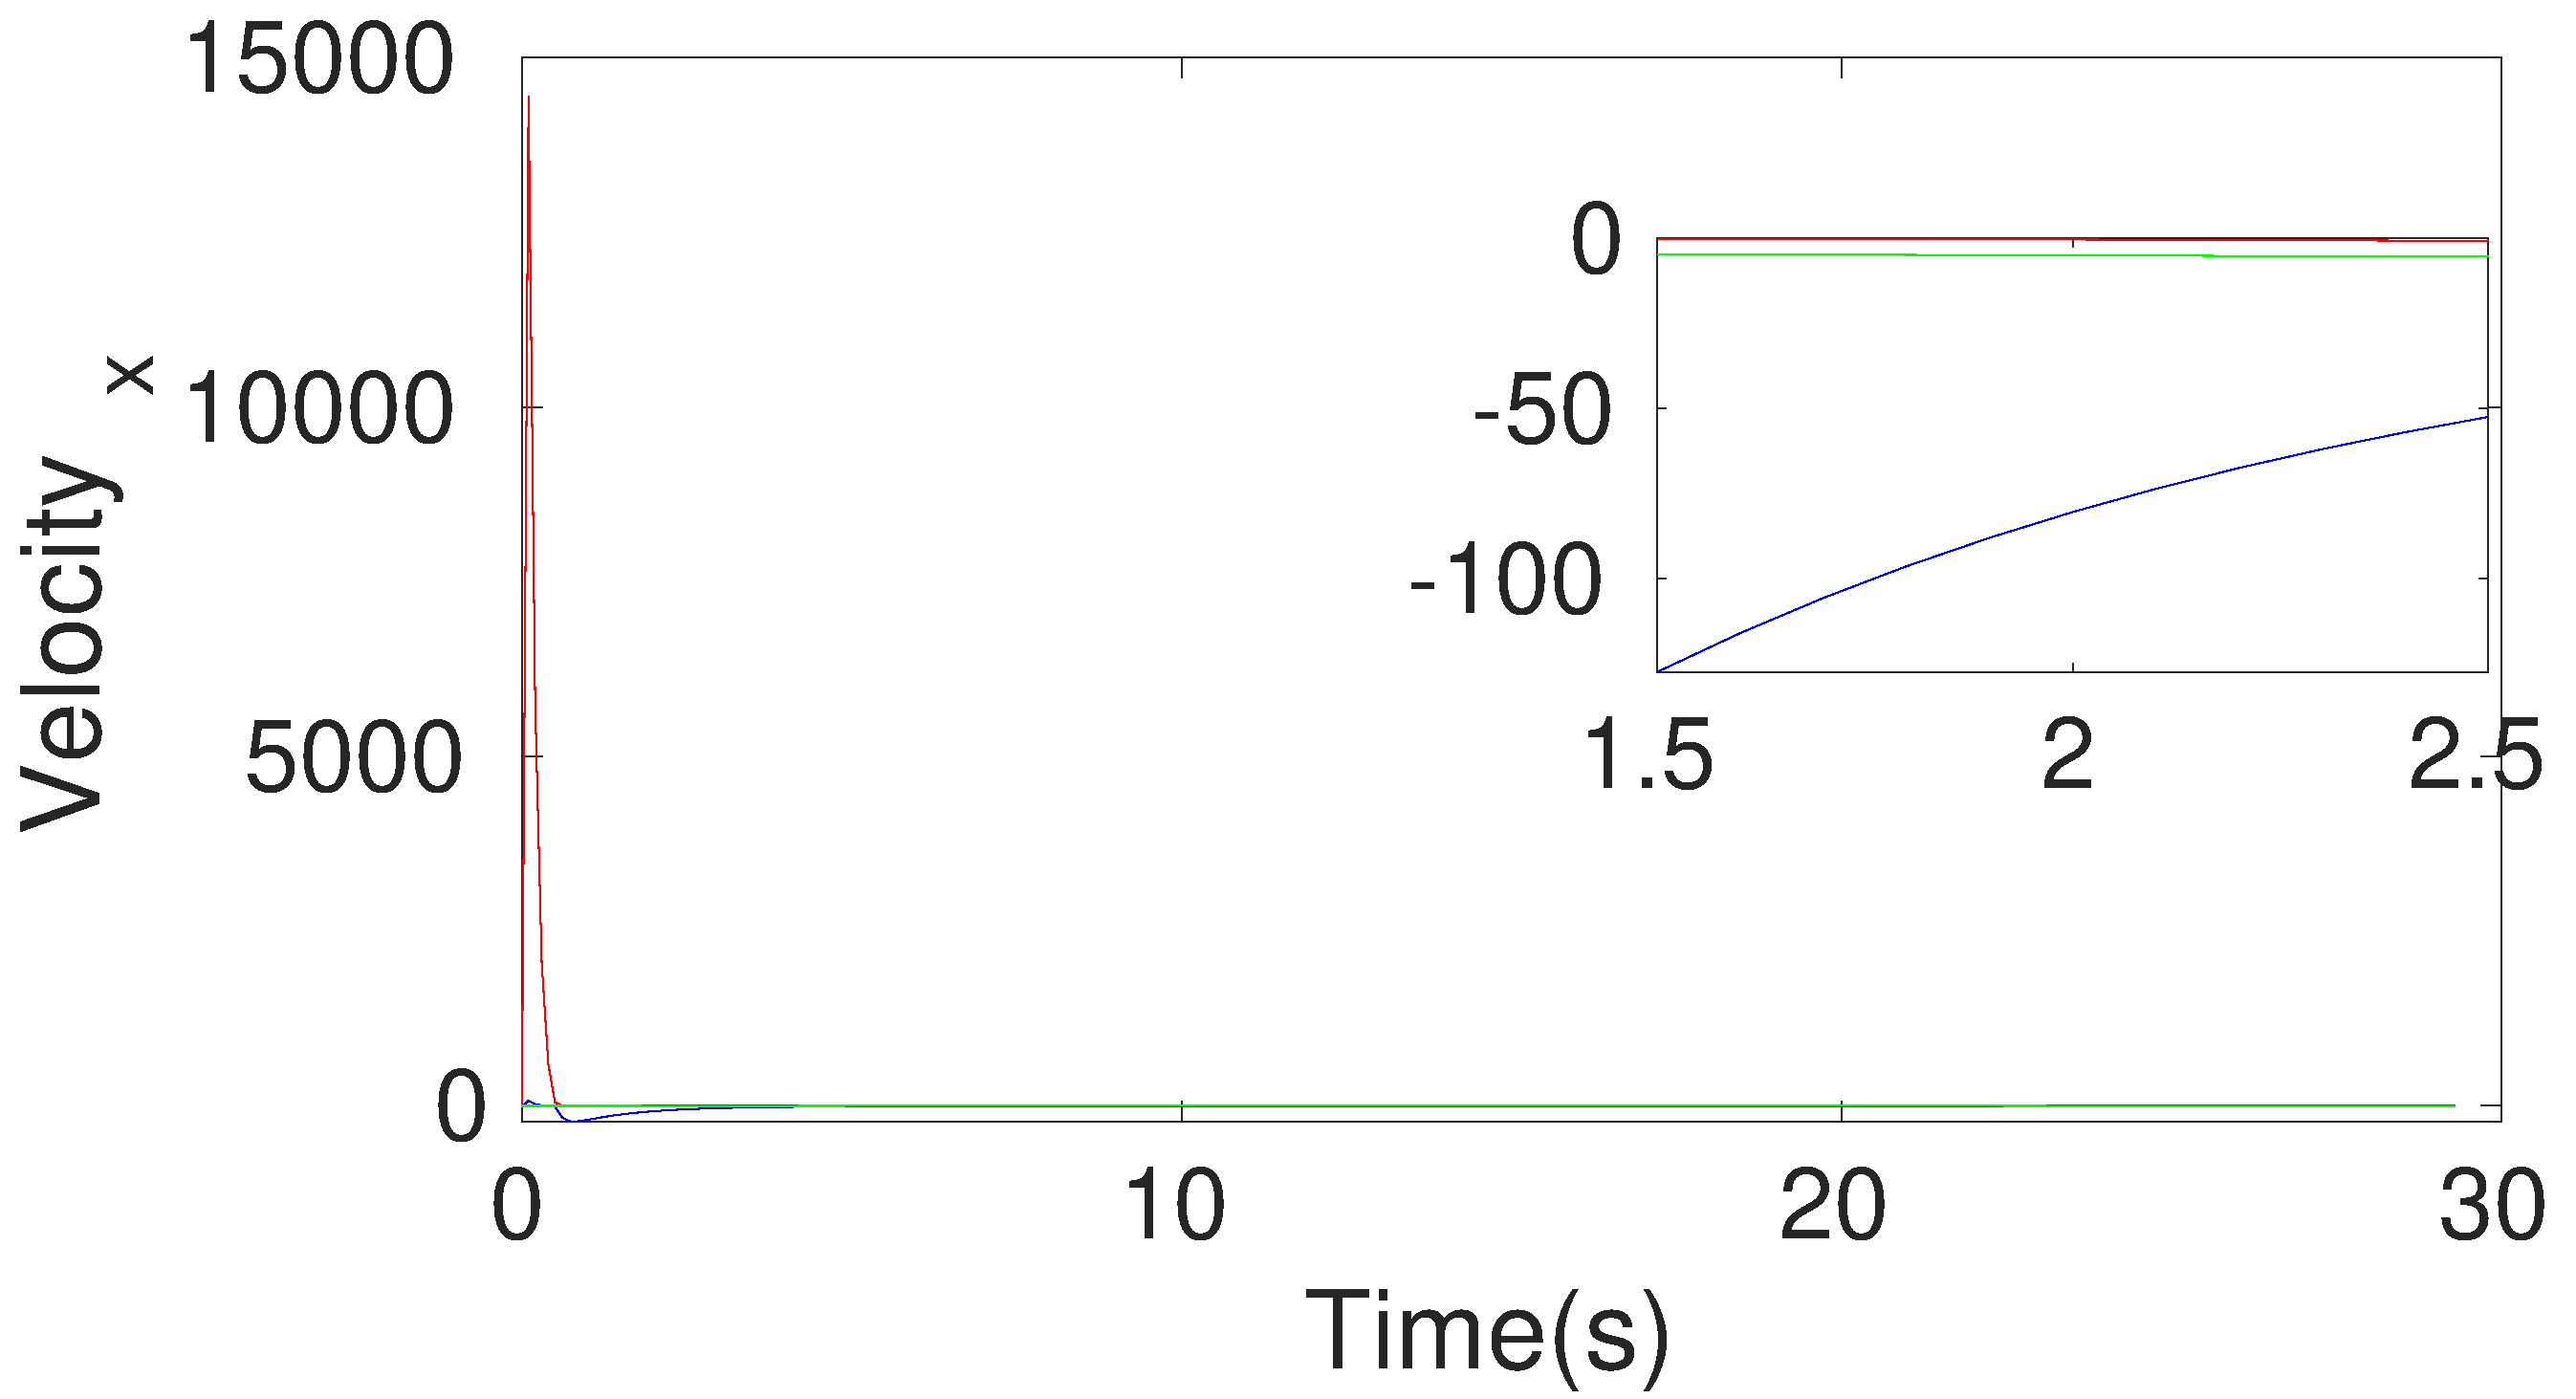
\includegraphics[width=\linewidth]{figures/HInf/s3caHInfVelocity_x}
\end{subfigure}
\begin{subfigure}{.5\linewidth}
\centering
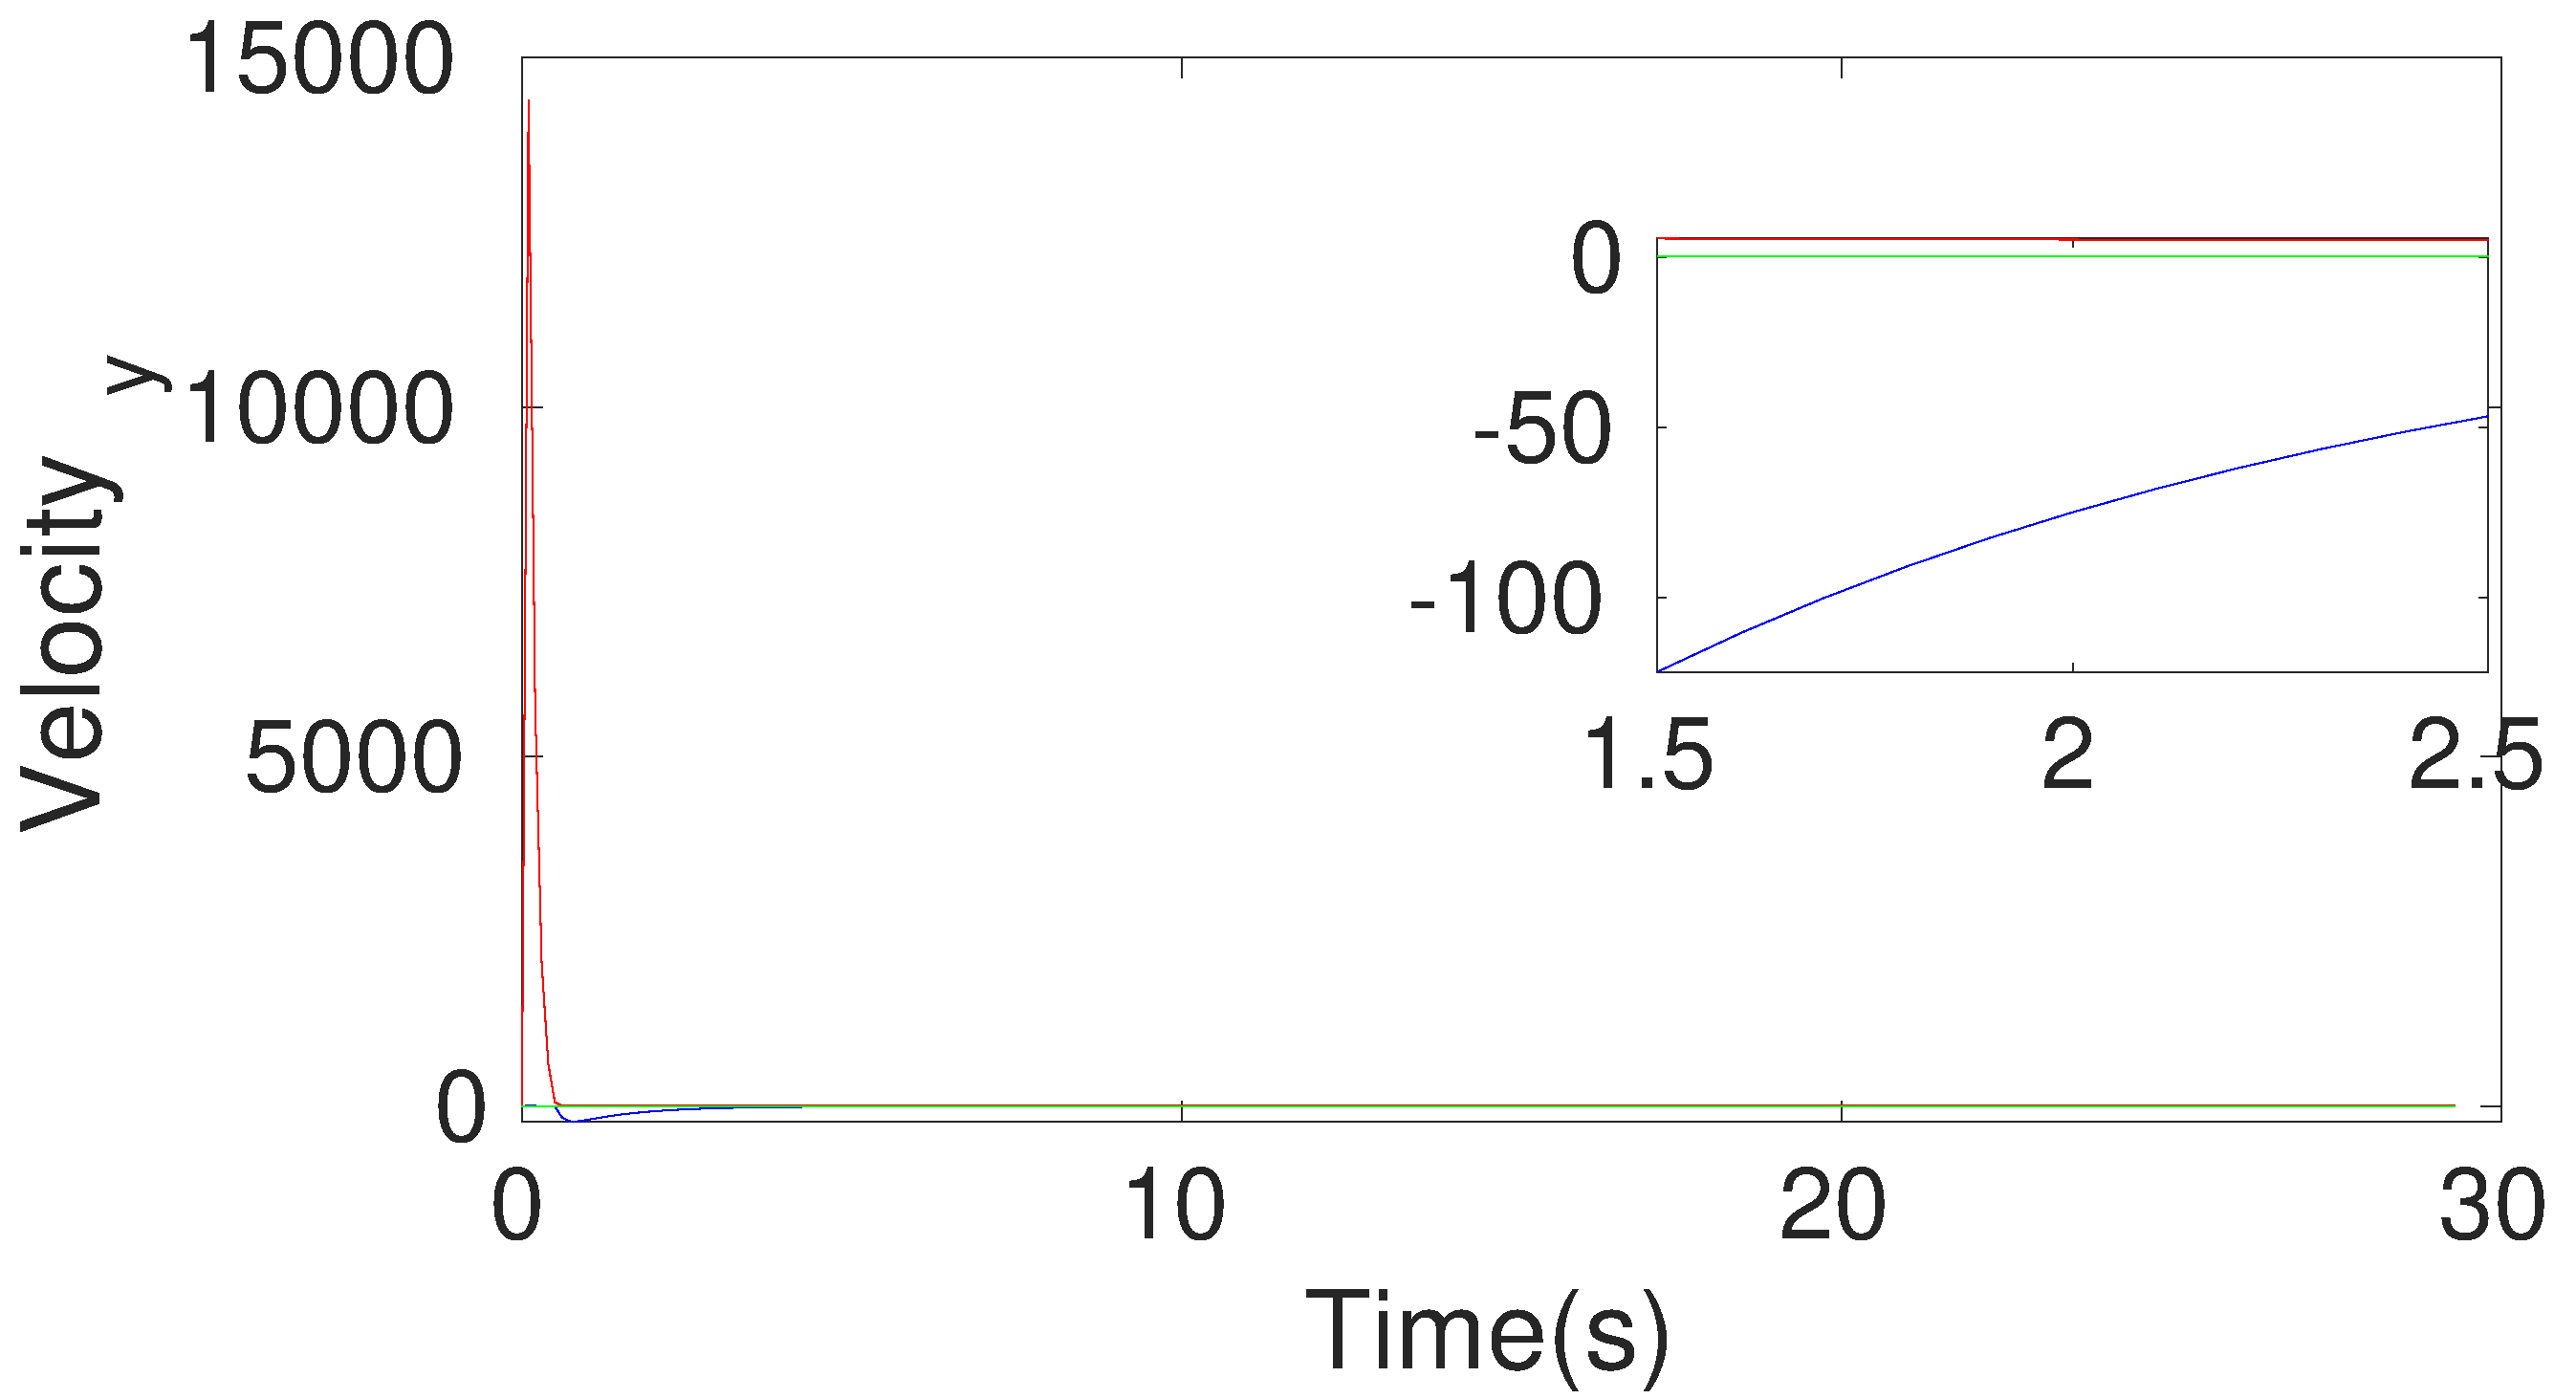
\includegraphics[width=\linewidth]{figures/HInf/s3caHInfVelocity_y}
\end{subfigure}
\begin{subfigure}{.5\linewidth}
\centering
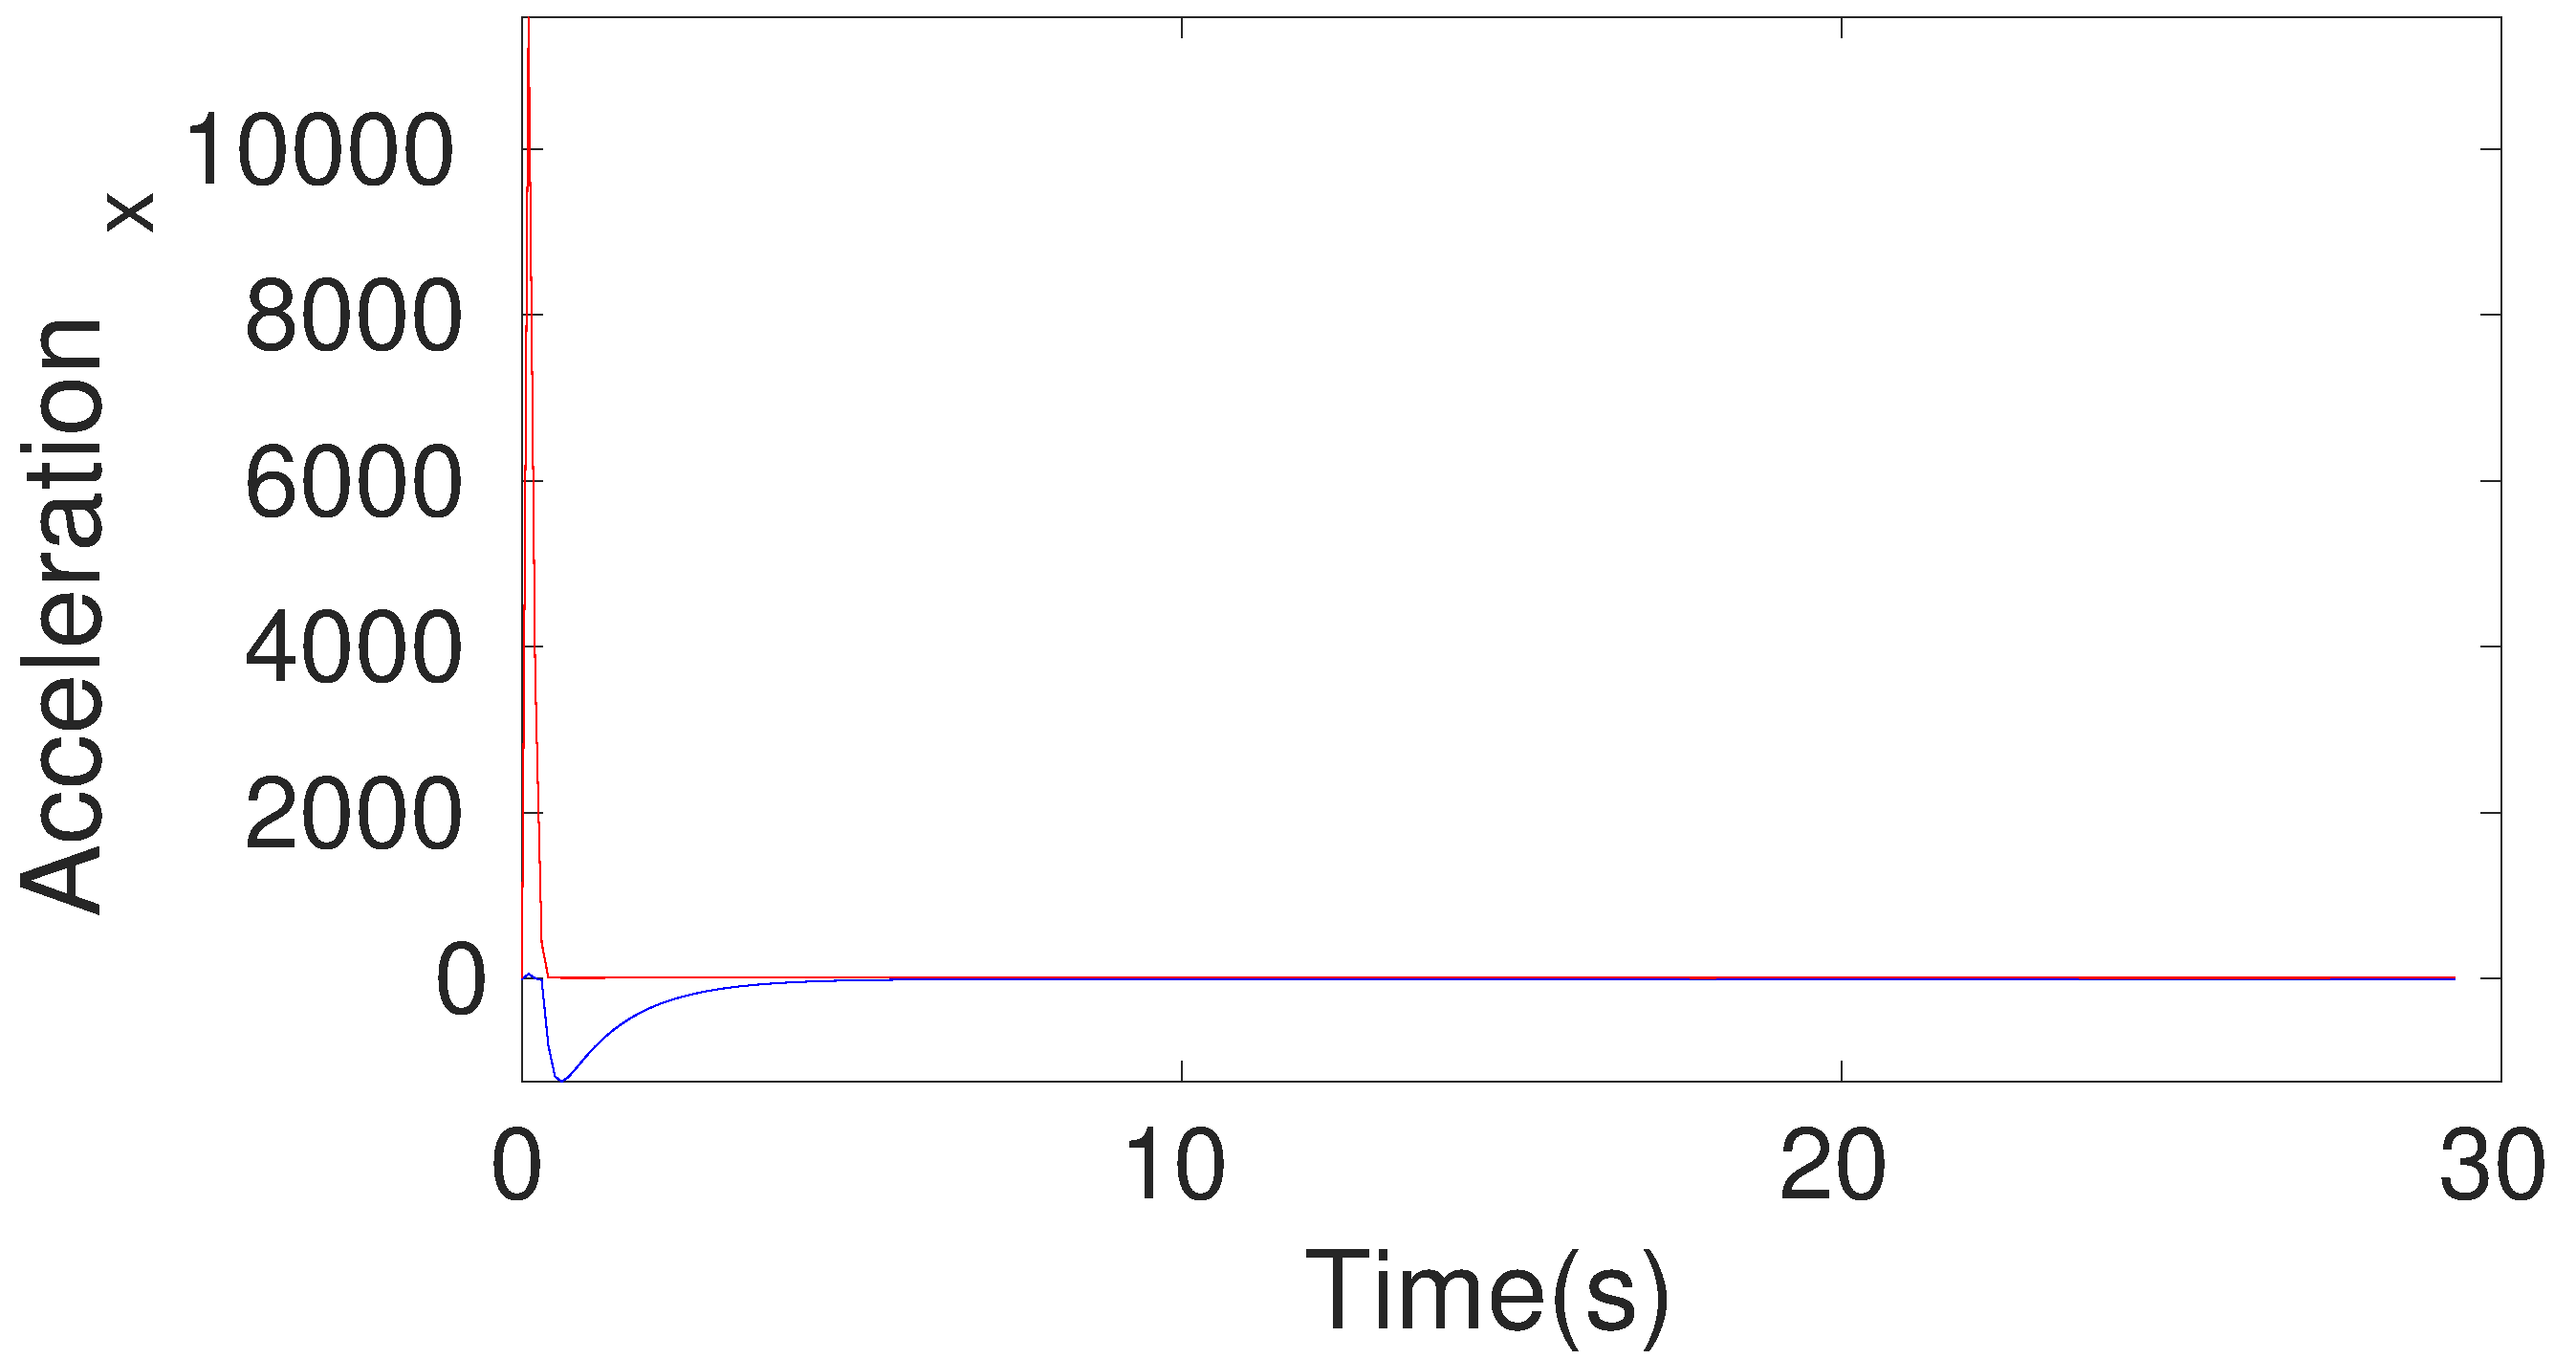
\includegraphics[width=\linewidth]{figures/HInf/s3caHInfAcceleration_x}
\end{subfigure}
\begin{subfigure}{.5\linewidth}
\centering
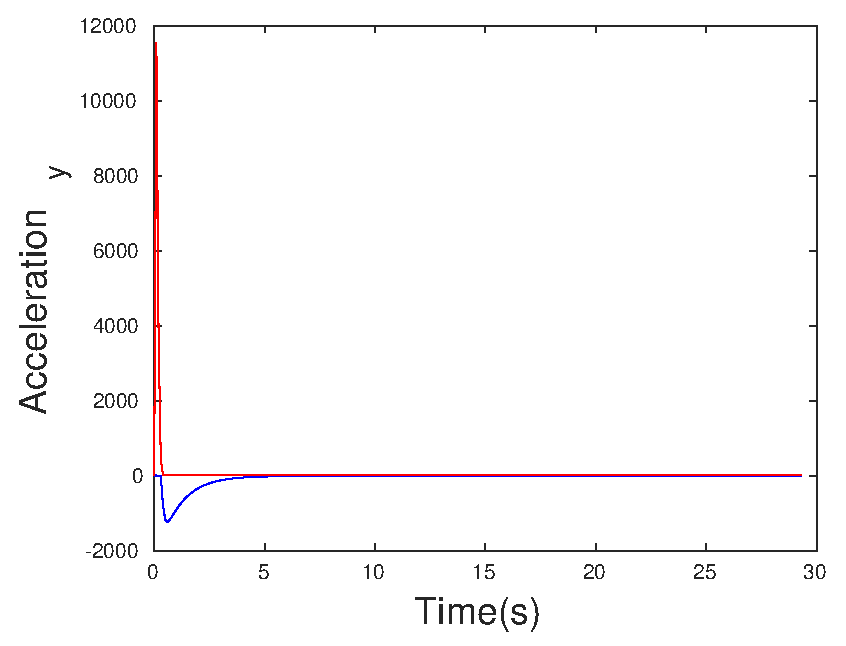
\includegraphics[width=\linewidth]{figures/HInf/s3caHInfAcceleration_y}
\end{subfigure}
\caption{Estimation using H-$\infty$ observer and the constant acceleration model}
\end{figure}

\begin{figure}[!h]
\hspace*{\fill} \includegraphics[scale=0.8]{figures/legend}\\\\
\begin{subfigure}{.5\linewidth}
\centering
\includegraphics[width=\linewidth]{figures/HInf/s3pmHInfX}
\end{subfigure}
\begin{subfigure}{.5\linewidth}
\centering
\includegraphics[width=\linewidth]{figures/HInf/s3pmHInfY}
\end{subfigure}
\begin{subfigure}{.5\linewidth}
\centering
\includegraphics[width=\linewidth]{figures/HInf/s3pmHInfVelocity_x}
\end{subfigure}
\begin{subfigure}{.5\linewidth}
\centering
\includegraphics[width=\linewidth]{figures/HInf/s3pmHInfVelocity_y}
\end{subfigure}
\begin{subfigure}{.5\linewidth}
\centering
\includegraphics[width=\linewidth]{figures/HInf/s3pmHInfAcceleration_x}
\end{subfigure}
\begin{subfigure}{.5\linewidth}
\centering
\includegraphics[width=\linewidth]{figures/HInf/s3pmHInfAcceleration_y}
\end{subfigure}
\caption{Estimation using H-$\infty$ observer and the point mass model}
\end{figure}

\FloatBarrier
\section{Rate of Change of Bounds}\label{eresult:rate}
\begin{figure}[!h]
\hspace*{\fill} \includegraphics[scale=0.8]{figures/ratelegend}\\\\
\begin{subfigure}{.5\linewidth}
\centering
\includegraphics[width=\linewidth]{figures/BoundChange/CV/cv_bound_changeX}
\end{subfigure}
\begin{subfigure}{.5\linewidth}
\centering
\includegraphics[width=\linewidth]{figures/BoundChange/CV/cv_bound_changeY}
\end{subfigure}
\begin{subfigure}{.5\linewidth}
\centering
\includegraphics[width=\linewidth]{figures/BoundChange/CV/cv_bound_changeVelocity_x}
\end{subfigure}
\begin{subfigure}{.5\linewidth}
\centering
\includegraphics[width=\linewidth]{figures/BoundChange/CV/cv_bound_changeVelocity_y}
\end{subfigure}
\caption{Rate of change of bounds using the constant velocity model}
\end{figure}

\begin{figure}[!h]
\hspace*{\fill} \includegraphics[scale=0.8]{figures/ratelegend}\\\\
\begin{subfigure}{.5\linewidth}
\centering
\includegraphics[width=\linewidth]{figures/BoundChange/CA/ca_bound_changeX}
\end{subfigure}
\begin{subfigure}{.5\linewidth}
\centering
\includegraphics[width=\linewidth]{figures/BoundChange/CA/ca_bound_changeY}
\end{subfigure}
\begin{subfigure}{.5\linewidth}
\centering
\includegraphics[width=\linewidth]{figures/BoundChange/CA/ca_bound_changeVelocity_x}
\end{subfigure}
\begin{subfigure}{.5\linewidth}
\centering
\includegraphics[width=\linewidth]{figures/BoundChange/CA/ca_bound_changeVelocity_y}
\end{subfigure}
\begin{subfigure}{.5\linewidth}
\centering
\includegraphics[width=\linewidth]{figures/BoundChange/CA/ca_bound_changeAcceleration_x}
\end{subfigure}
\begin{subfigure}{.5\linewidth}
\centering
\includegraphics[width=\linewidth]{figures/BoundChange/CA/ca_bound_changeAcceleration_y}
\end{subfigure}
\caption{Rate of change of bounds using the constant acceleration model}
\end{figure}

\begin{figure}[!h]
\hspace*{\fill} \includegraphics[scale=0.8]{figures/ratelegend}\\\\
\begin{subfigure}{.5\linewidth}
\centering
\includegraphics[width=\linewidth]{figures/BoundChange/PM/pm_bound_changeX}
\end{subfigure}
\begin{subfigure}{.5\linewidth}
\centering
\includegraphics[width=\linewidth]{figures/BoundChange/PM/pm_bound_changeY}
\end{subfigure}
\begin{subfigure}{.5\linewidth}
\centering
\includegraphics[width=\linewidth]{figures/BoundChange/PM/pm_bound_changeVelocity_x}
\end{subfigure}
\begin{subfigure}{.5\linewidth}
\centering
\includegraphics[width=\linewidth]{figures/BoundChange/PM/pm_bound_changeVelocity_y}
\end{subfigure}
\begin{subfigure}{.5\linewidth}
\centering
\includegraphics[width=\linewidth]{figures/BoundChange/PM/pm_bound_changeAcceleration_x}
\end{subfigure}
\begin{subfigure}{.5\linewidth}
\centering
\includegraphics[width=\linewidth]{figures/BoundChange/PM/pm_bound_changeAcceleration_y}
\end{subfigure}
\caption{Rate of change of bounds using the point-mass model}
\end{figure}
\pagebreak
